\documentclass[twoside]{book}

% Packages required by doxygen
\usepackage{calc}
\usepackage{doxygen}
\usepackage{graphicx}
\usepackage[utf8]{inputenc}
\usepackage{makeidx}
\usepackage{multicol}
\usepackage{multirow}
\usepackage{fixltx2e}
\PassOptionsToPackage{warn}{textcomp}
\usepackage{textcomp}
\usepackage[nointegrals]{wasysym}
\usepackage[table]{xcolor}

% NLS support packages
\usepackage[french]{babel}

% Font selection
\usepackage[T1]{fontenc}
\usepackage{mathptmx}
\usepackage[scaled=.90]{helvet}
\usepackage{courier}
\usepackage{amssymb}
\usepackage{sectsty}
\renewcommand{\familydefault}{\sfdefault}
\allsectionsfont{%
  \fontseries{bc}\selectfont%
  \color{darkgray}%
}
\renewcommand{\DoxyLabelFont}{%
  \fontseries{bc}\selectfont%
  \color{darkgray}%
}
\newcommand{\+}{\discretionary{\mbox{\scriptsize$\hookleftarrow$}}{}{}}

% Page & text layout
\usepackage{geometry}
\geometry{%
  a4paper,%
  top=2.5cm,%
  bottom=2.5cm,%
  left=2.5cm,%
  right=2.5cm%
}
\tolerance=750
\hfuzz=15pt
\hbadness=750
\setlength{\emergencystretch}{15pt}
\setlength{\parindent}{0cm}
\setlength{\parskip}{0.2cm}
\makeatletter
\renewcommand{\paragraph}{%
  \@startsection{paragraph}{4}{0ex}{-1.0ex}{1.0ex}{%
    \normalfont\normalsize\bfseries\SS@parafont%
  }%
}
\renewcommand{\subparagraph}{%
  \@startsection{subparagraph}{5}{0ex}{-1.0ex}{1.0ex}{%
    \normalfont\normalsize\bfseries\SS@subparafont%
  }%
}
\makeatother

% Headers & footers
\usepackage{fancyhdr}
\pagestyle{fancyplain}
\fancyhead[LE]{\fancyplain{}{\bfseries\thepage}}
\fancyhead[CE]{\fancyplain{}{}}
\fancyhead[RE]{\fancyplain{}{\bfseries\leftmark}}
\fancyhead[LO]{\fancyplain{}{\bfseries\rightmark}}
\fancyhead[CO]{\fancyplain{}{}}
\fancyhead[RO]{\fancyplain{}{\bfseries\thepage}}
\fancyfoot[LE]{\fancyplain{}{}}
\fancyfoot[CE]{\fancyplain{}{}}
\fancyfoot[RE]{\fancyplain{}{\bfseries\scriptsize Généré le Lundi 26 Mai 2014 23\+:22\+:57 pour Simulation d'un gaz parfait par Doxygen }}
\fancyfoot[LO]{\fancyplain{}{\bfseries\scriptsize Généré le Lundi 26 Mai 2014 23\+:22\+:57 pour Simulation d'un gaz parfait par Doxygen }}
\fancyfoot[CO]{\fancyplain{}{}}
\fancyfoot[RO]{\fancyplain{}{}}
\renewcommand{\footrulewidth}{0.4pt}
\renewcommand{\chaptermark}[1]{%
  \markboth{#1}{}%
}
\renewcommand{\sectionmark}[1]{%
  \markright{\thesection\ #1}%
}

% Indices & bibliography
\usepackage{natbib}
\usepackage[titles]{tocloft}
\setcounter{tocdepth}{3}
\setcounter{secnumdepth}{5}
\makeindex

% Custom commands
\newcommand{\clearemptydoublepage}{%
  \newpage{\pagestyle{empty}\cleardoublepage}%
}


%===== C O N T E N T S =====

\begin{document}

% Titlepage & ToC
\pagenumbering{roman}
\begin{titlepage}
\vspace*{7cm}
\begin{center}%
{\Large Simulation d'un gaz parfait \\[1ex]\large 2.\+0 }\\
\vspace*{1cm}
{\large Généré par Doxygen 1.8.7}\\
\vspace*{0.5cm}
{\small Lundi 26 Mai 2014 23:22:57}\\
\end{center}
\end{titlepage}
\clearemptydoublepage
\tableofcontents
\clearemptydoublepage
\pagenumbering{arabic}

%--- Begin generated contents ---
\chapter{Index hiérarchique}
\section{Hiérarchie des classes}
Cette liste d'héritage est classée approximativement par ordre alphabétique \+:\begin{DoxyCompactList}
\item \contentsline{section}{Dessinable}{\pageref{class_dessinable}}{}
\begin{DoxyCompactList}
\item \contentsline{section}{Canon}{\pageref{class_canon}}{}
\item \contentsline{section}{Enceinte}{\pageref{class_enceinte}}{}
\item \contentsline{section}{Particule}{\pageref{class_particule}}{}
\begin{DoxyCompactList}
\item \contentsline{section}{G\+L\+Argon}{\pageref{class_g_l_argon}}{}
\item \contentsline{section}{G\+L\+Fluor}{\pageref{class_g_l_fluor}}{}
\item \contentsline{section}{G\+L\+Helium}{\pageref{class_g_l_helium}}{}
\item \contentsline{section}{G\+L\+Neon}{\pageref{class_g_l_neon}}{}
\item \contentsline{section}{T\+X\+T\+Argon}{\pageref{class_t_x_t_argon}}{}
\item \contentsline{section}{T\+X\+T\+Helium}{\pageref{class_t_x_t_helium}}{}
\item \contentsline{section}{T\+X\+T\+Neon}{\pageref{class_t_x_t_neon}}{}
\end{DoxyCompactList}
\item \contentsline{section}{Systeme}{\pageref{class_systeme}}{}
\end{DoxyCompactList}
\item \contentsline{section}{Generateur\+Aleatoire}{\pageref{class_generateur_aleatoire}}{}
\item \contentsline{section}{T\+X\+T\+Argon\+:\+:h}{\pageref{class_t_x_t_argon_1_1h}}{}
\item \contentsline{section}{T\+X\+T\+Neon\+:\+:h}{\pageref{class_t_x_t_neon_1_1h}}{}
\item \contentsline{section}{T\+X\+T\+Helium\+:\+:h}{\pageref{class_t_x_t_helium_1_1h}}{}
\item \contentsline{section}{Vecteur}{\pageref{class_vecteur}}{}
\item wx\+App\begin{DoxyCompactList}
\item \contentsline{section}{G\+U\+I}{\pageref{class_g_u_i}}{}
\end{DoxyCompactList}
\item wx\+Frame\begin{DoxyCompactList}
\item \contentsline{section}{Fenetre}{\pageref{class_fenetre}}{}
\end{DoxyCompactList}
\item wx\+G\+L\+Canvas\begin{DoxyCompactList}
\item \contentsline{section}{Vue\+\_\+\+Open\+G\+L}{\pageref{class_vue___open_g_l}}{}
\end{DoxyCompactList}
\end{DoxyCompactList}

\chapter{Index des classes}
\section{Liste des classes}
Liste des classes, structures, unions et interfaces avec une brève description \+:\begin{DoxyCompactList}
\item\contentsline{section}{{\bf Canon} \\*Prototype de la classe \doxyref{Canon}{p.}{class_canon} }{\pageref{class_canon}}{}
\item\contentsline{section}{{\bf Dessinable} }{\pageref{class_dessinable}}{}
\item\contentsline{section}{{\bf Enceinte} }{\pageref{class_enceinte}}{}
\item\contentsline{section}{{\bf Fenetre} }{\pageref{class_fenetre}}{}
\item\contentsline{section}{{\bf Generateur\+Aleatoire} \\*Représente des objets capables de générer des nombres aléatoires }{\pageref{class_generateur_aleatoire}}{}
\item\contentsline{section}{{\bf G\+L\+Argon} \\*Prototype de la classe \doxyref{G\+L\+Argon}{p.}{class_g_l_argon} }{\pageref{class_g_l_argon}}{}
\item\contentsline{section}{{\bf G\+L\+Fluor} \\*Prototype de la classe G\+Lluor }{\pageref{class_g_l_fluor}}{}
\item\contentsline{section}{{\bf G\+L\+Helium} \\*Prototype de la classe \doxyref{G\+L\+Helium}{p.}{class_g_l_helium} }{\pageref{class_g_l_helium}}{}
\item\contentsline{section}{{\bf G\+L\+Neon} \\*Prototype de la classe \doxyref{G\+L\+Neon}{p.}{class_g_l_neon} }{\pageref{class_g_l_neon}}{}
\item\contentsline{section}{{\bf G\+U\+I} \\*Application principale }{\pageref{class_g_u_i}}{}
\item\contentsline{section}{{\bf T\+X\+T\+Argon\+::h} \\*Représente des atomes d'Argon (version texte) }{\pageref{class_t_x_t_argon_1_1h}}{}
\item\contentsline{section}{{\bf T\+X\+T\+Neon\+::h} \\*Représente des atomes de Neon (version texte) }{\pageref{class_t_x_t_neon_1_1h}}{}
\item\contentsline{section}{{\bf T\+X\+T\+Helium\+::h} \\*Représente des atomes d'Helium (version texte) }{\pageref{class_t_x_t_helium_1_1h}}{}
\item\contentsline{section}{{\bf Particule} \\*Classe mère dont hérite toutes les classes de type \+: T\+X\+T\+Nom et G\+L\+Nom Représentation d'une particule (ici version graphique) }{\pageref{class_particule}}{}
\item\contentsline{section}{{\bf Systeme} \\*Permet de créer, de dessiner et de faire évoluer des objets de type \doxyref{Systeme}{p.}{class_systeme} formés d'une enceinte et de particules }{\pageref{class_systeme}}{}
\item\contentsline{section}{{\bf T\+X\+T\+Argon} }{\pageref{class_t_x_t_argon}}{}
\item\contentsline{section}{{\bf T\+X\+T\+Helium} }{\pageref{class_t_x_t_helium}}{}
\item\contentsline{section}{{\bf T\+X\+T\+Neon} }{\pageref{class_t_x_t_neon}}{}
\item\contentsline{section}{{\bf Vecteur} \\*Prototype de la classe \doxyref{Vecteur}{p.}{class_vecteur} }{\pageref{class_vecteur}}{}
\item\contentsline{section}{{\bf Vue\+\_\+\+Open\+G\+L} \\*Prototype de la classe \doxyref{Vue\+\_\+\+Open\+G\+L}{p.}{class_vue___open_g_l} }{\pageref{class_vue___open_g_l}}{}
\end{DoxyCompactList}

\chapter{Index des fichiers}
\section{Liste des fichiers}
Liste de tous les fichiers avec une brève description \+:\begin{DoxyCompactList}
\item\contentsline{section}{/\+Users/burkhard/\+Dropbox/projet d'info/maximilian-\/g065/\+Simulation d'un gaz parfait/{\bf Canon.\+cc} \\*Fichier permettant la définition de la classe \doxyref{Canon}{p.}{class_canon} }{\pageref{_canon_8cc}}{}
\item\contentsline{section}{/\+Users/burkhard/\+Dropbox/projet d'info/maximilian-\/g065/\+Simulation d'un gaz parfait/{\bf Canon.\+h} \\*Est la classe qui contient l'objet enceinte qui est la boîte où seront nos particules }{\pageref{_canon_8h}}{}
\item\contentsline{section}{/\+Users/burkhard/\+Dropbox/projet d'info/maximilian-\/g065/\+Simulation d'un gaz parfait/{\bf Dessinable.\+h} \\*Est la super-\/classe avec une méthode dessine qui permet d'avoir une spécialisation pour chaque type d'objet }{\pageref{_dessinable_8h}}{}
\item\contentsline{section}{/\+Users/burkhard/\+Dropbox/projet d'info/maximilian-\/g065/\+Simulation d'un gaz parfait/{\bf Enceinte.\+cc} \\*Fichier permettant la définition de la classe enceinte }{\pageref{_enceinte_8cc}}{}
\item\contentsline{section}{/\+Users/burkhard/\+Dropbox/projet d'info/maximilian-\/g065/\+Simulation d'un gaz parfait/{\bf Enceinte.\+h} \\*Est la classe qui contient l'objet enceinte qui est la boîte où seront nos particules }{\pageref{_enceinte_8h}}{}
\item\contentsline{section}{/\+Users/burkhard/\+Dropbox/projet d'info/maximilian-\/g065/\+Simulation d'un gaz parfait/{\bf Fenetre.\+cc} \\*Est la définition de la classe fenêtre en Open\+G\+L }{\pageref{_fenetre_8cc}}{}
\item\contentsline{section}{/\+Users/burkhard/\+Dropbox/projet d'info/maximilian-\/g065/\+Simulation d'un gaz parfait/{\bf Fenetre.\+h} \\*Est le prototype de la classe fenetre qui permettra de créer une fentre contenant notre application }{\pageref{_fenetre_8h}}{}
\item\contentsline{section}{/\+Users/burkhard/\+Dropbox/projet d'info/maximilian-\/g065/\+Simulation d'un gaz parfait/{\bf Generateur\+Aleatoire.\+cc} \\*Définition de la classe qui permet de générer des nombres aléatoires }{\pageref{_generateur_aleatoire_8cc}}{}
\item\contentsline{section}{/\+Users/burkhard/\+Dropbox/projet d'info/maximilian-\/g065/\+Simulation d'un gaz parfait/{\bf Generateur\+Aleatoire.\+h} \\*Prototype de la classe qui permet de générer des nombres aléatoires }{\pageref{_generateur_aleatoire_8h}}{}
\item\contentsline{section}{/\+Users/burkhard/\+Dropbox/projet d'info/maximilian-\/g065/\+Simulation d'un gaz parfait/{\bf G\+L\+Argon.\+cc} \\*Est la définition de la classe de la particule argon en Open\+G\+L }{\pageref{_g_l_argon_8cc}}{}
\item\contentsline{section}{/\+Users/burkhard/\+Dropbox/projet d'info/maximilian-\/g065/\+Simulation d'un gaz parfait/{\bf G\+L\+Argon.\+h} \\*Est le prototype de la classe de la particule argon en Open\+G\+L }{\pageref{_g_l_argon_8h}}{}
\item\contentsline{section}{/\+Users/burkhard/\+Dropbox/projet d'info/maximilian-\/g065/\+Simulation d'un gaz parfait/{\bf G\+L\+Fluor.\+cc} \\*Est la définition de la classe de la particule fluor en Open\+G\+L qui a en plus une mémorisation et affichage de la trajectoire }{\pageref{_g_l_fluor_8cc}}{}
\item\contentsline{section}{/\+Users/burkhard/\+Dropbox/projet d'info/maximilian-\/g065/\+Simulation d'un gaz parfait/{\bf G\+L\+Fluor.\+h} \\*Est le prototype de la classe de la particule fluor en Open\+G\+L qui a en plus une mémorisation et affichage de la trajectoire }{\pageref{_g_l_fluor_8h}}{}
\item\contentsline{section}{/\+Users/burkhard/\+Dropbox/projet d'info/maximilian-\/g065/\+Simulation d'un gaz parfait/{\bf G\+L\+Helium.\+cc} \\*Est la définition de la classe de la particule Helium en Open\+G\+L }{\pageref{_g_l_helium_8cc}}{}
\item\contentsline{section}{/\+Users/burkhard/\+Dropbox/projet d'info/maximilian-\/g065/\+Simulation d'un gaz parfait/{\bf G\+L\+Helium.\+h} \\*Est le prototype de la classe de la particule Helium en Open\+G\+L }{\pageref{_g_l_helium_8h}}{}
\item\contentsline{section}{/\+Users/burkhard/\+Dropbox/projet d'info/maximilian-\/g065/\+Simulation d'un gaz parfait/{\bf G\+L\+Neon.\+cc} \\*Est la définition de la classe de la particule Néon en Open\+G\+L }{\pageref{_g_l_neon_8cc}}{}
\item\contentsline{section}{/\+Users/burkhard/\+Dropbox/projet d'info/maximilian-\/g065/\+Simulation d'un gaz parfait/{\bf G\+L\+Neon.\+h} \\*Est le prototype de la classe de la particule néon en Open\+G\+L }{\pageref{_g_l_neon_8h}}{}
\item\contentsline{section}{/\+Users/burkhard/\+Dropbox/projet d'info/maximilian-\/g065/\+Simulation d'un gaz parfait/{\bf G\+U\+I.\+cc} \\*Est la définition de l'application princpal qui lance tout le programme }{\pageref{_g_u_i_8cc}}{}
\item\contentsline{section}{/\+Users/burkhard/\+Dropbox/projet d'info/maximilian-\/g065/\+Simulation d'un gaz parfait/{\bf G\+U\+I.\+h} \\*Est le prototype de l'application princpal qui lance tout le programme }{\pageref{_g_u_i_8h}}{}
\item\contentsline{section}{/\+Users/burkhard/\+Dropbox/projet d'info/maximilian-\/g065/\+Simulation d'un gaz parfait/{\bf Particule.\+cc} \\*Définition de la classe mère \doxyref{Particule}{p.}{class_particule} }{\pageref{_particule_8cc}}{}
\item\contentsline{section}{/\+Users/burkhard/\+Dropbox/projet d'info/maximilian-\/g065/\+Simulation d'un gaz parfait/{\bf Particule.\+h} \\*Prototype de la classe mère \doxyref{Particule}{p.}{class_particule} }{\pageref{_particule_8h}}{}
\item\contentsline{section}{/\+Users/burkhard/\+Dropbox/projet d'info/maximilian-\/g065/\+Simulation d'un gaz parfait/{\bf Systeme.\+cc} \\*Définition de la classe \doxyref{Systeme}{p.}{class_systeme} (objet formé d'une enceinte et de particules) }{\pageref{_systeme_8cc}}{}
\item\contentsline{section}{/\+Users/burkhard/\+Dropbox/projet d'info/maximilian-\/g065/\+Simulation d'un gaz parfait/{\bf Systeme.\+h} \\*Prototype de la classe de la classe \doxyref{Systeme}{p.}{class_systeme} (objet formé d'une enceinte et de particules) }{\pageref{_systeme_8h}}{}
\item\contentsline{section}{/\+Users/burkhard/\+Dropbox/projet d'info/maximilian-\/g065/\+Simulation d'un gaz parfait/{\bf T\+X\+T\+Argon.\+cc} \\*Définition de la classe de la particule Argon en version texte }{\pageref{_t_x_t_argon_8cc}}{}
\item\contentsline{section}{/\+Users/burkhard/\+Dropbox/projet d'info/maximilian-\/g065/\+Simulation d'un gaz parfait/{\bf T\+X\+T\+Argon.\+h} \\*Prototype de la classe de la particule Argon en version texte }{\pageref{_t_x_t_argon_8h}}{}
\item\contentsline{section}{/\+Users/burkhard/\+Dropbox/projet d'info/maximilian-\/g065/\+Simulation d'un gaz parfait/{\bf T\+X\+T\+Helium.\+cc} \\*Définition de la classe de la particule Helium en version texte }{\pageref{_t_x_t_helium_8cc}}{}
\item\contentsline{section}{/\+Users/burkhard/\+Dropbox/projet d'info/maximilian-\/g065/\+Simulation d'un gaz parfait/{\bf T\+X\+T\+Helium.\+h} \\*Prototype de la classe de la particule Helium en version texte }{\pageref{_t_x_t_helium_8h}}{}
\item\contentsline{section}{/\+Users/burkhard/\+Dropbox/projet d'info/maximilian-\/g065/\+Simulation d'un gaz parfait/{\bf T\+X\+T\+Neon.\+cc} \\*Définition de la classe de la particule Neon en version texte }{\pageref{_t_x_t_neon_8cc}}{}
\item\contentsline{section}{/\+Users/burkhard/\+Dropbox/projet d'info/maximilian-\/g065/\+Simulation d'un gaz parfait/{\bf T\+X\+T\+Neon.\+h} }{\pageref{_t_x_t_neon_8h}}{}
\item\contentsline{section}{/\+Users/burkhard/\+Dropbox/projet d'info/maximilian-\/g065/\+Simulation d'un gaz parfait/{\bf Vecteur.\+cc} \\*Est la définition de la classe qui nous pourmet de gérer la position et la vitesse de nos particules mais aussi de tous l'espace qui les entours }{\pageref{_vecteur_8cc}}{}
\item\contentsline{section}{/\+Users/burkhard/\+Dropbox/projet d'info/maximilian-\/g065/\+Simulation d'un gaz parfait/{\bf Vecteur.\+h} \\*Est le prototype de la classe qui nous pourmet de gérer la position et la vitesse de nos particules mais aussi de tous l'espace qui les entours }{\pageref{_vecteur_8h}}{}
\item\contentsline{section}{/\+Users/burkhard/\+Dropbox/projet d'info/maximilian-\/g065/\+Simulation d'un gaz parfait/{\bf Vue\+\_\+\+Open\+G\+L.\+cc} }{\pageref{_vue___open_g_l_8cc}}{}
\item\contentsline{section}{/\+Users/burkhard/\+Dropbox/projet d'info/maximilian-\/g065/\+Simulation d'un gaz parfait/{\bf Vue\+\_\+\+Open\+G\+L.\+h} }{\pageref{_vue___open_g_l_8h}}{}
\end{DoxyCompactList}

\chapter{Documentation des classes}
\section{Référence de la classe Canon}
\label{class_canon}\index{Canon@{Canon}}


Prototype de la classe \doxyref{Canon}{p.}{class_canon}.  




{\ttfamily \#include $<$Canon.\+h$>$}

Graphe d'héritage de Canon\+:\begin{figure}[H]
\begin{center}
\leavevmode
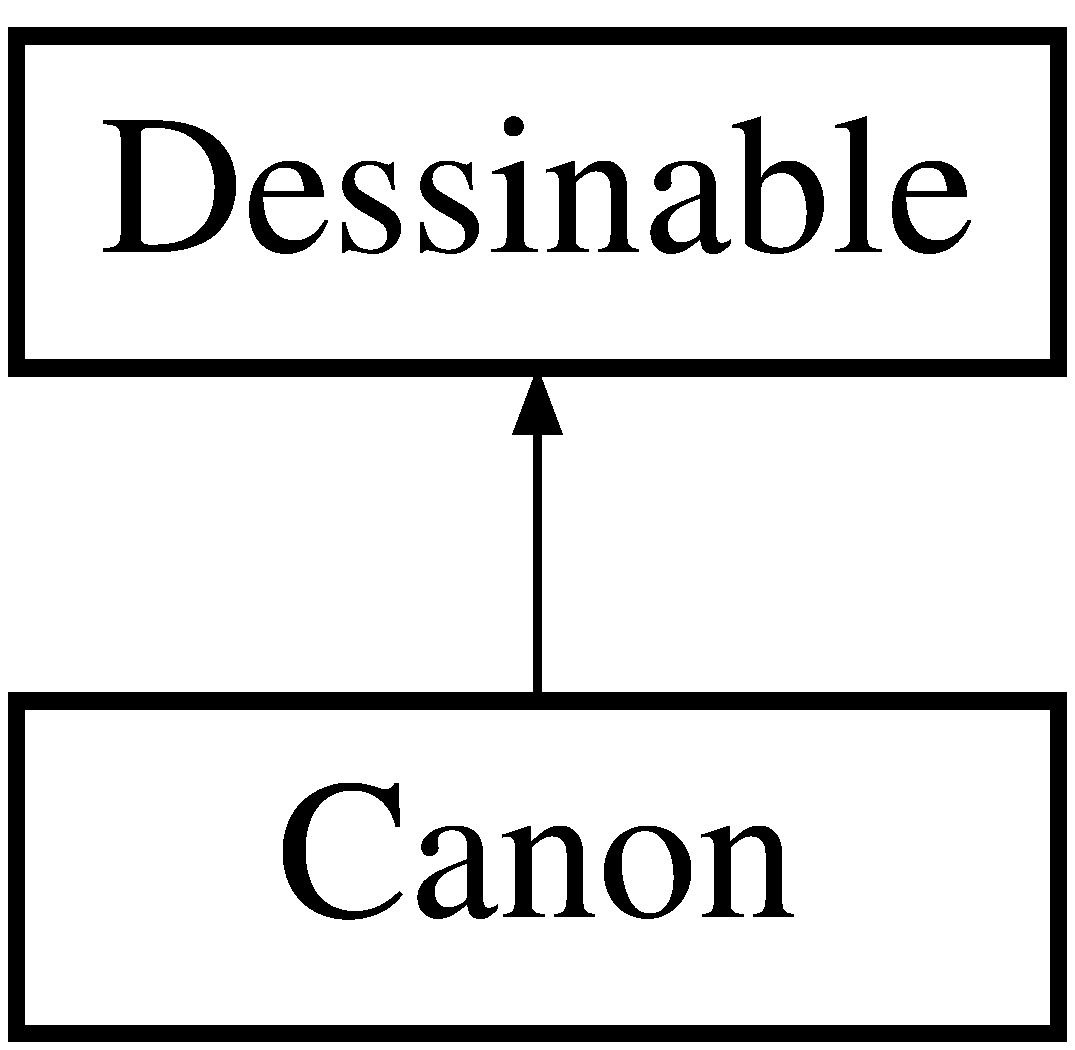
\includegraphics[height=2.000000cm]{class_canon}
\end{center}
\end{figure}
\subsection*{Fonctions membres publiques}
\begin{DoxyCompactItemize}
\item 
{\bf Canon} ()
\begin{DoxyCompactList}\small\item\em Constructeur sans paramètre. \end{DoxyCompactList}\item 
{\bf $\sim$\+Canon} ()
\begin{DoxyCompactList}\small\item\em Destructeur de \doxyref{Canon}{p.}{class_canon} qui détruit chacune des parties du canons. \end{DoxyCompactList}\item 
virtual void {\bf dessine} () const 
\begin{DoxyCompactList}\small\item\em Prototype de la méthode dessine en Open\+G\+L. \end{DoxyCompactList}\end{DoxyCompactItemize}


\subsection{Description détaillée}
Prototype de la classe \doxyref{Canon}{p.}{class_canon}. 

Cette classe est celle qui permet de créer et de dessiner un canon à particule. Nous avons dessidé de le faire car nous voulions ajouté des particules au systeme.

Elle hérite de dessinable car il fallait avoir une méthode dessine et cela respecte le bonne programmation car on utilise l'héritage. 

Définition à la ligne {\bf 29} du fichier {\bf Canon.\+h}.



\subsection{Documentation des constructeurs et destructeur}
\index{Canon@{Canon}!Canon@{Canon}}
\index{Canon@{Canon}!Canon@{Canon}}
\subsubsection[{Canon}]{\setlength{\rightskip}{0pt plus 5cm}Canon\+::\+Canon (
\begin{DoxyParamCaption}
{}
\end{DoxyParamCaption}
)}\label{class_canon_af33c1f50936632b864bb9af1fdd20453}


Constructeur sans paramètre. 

Constructeur de la classe du \doxyref{Canon}{p.}{class_canon} qui initialise la longueur et le rayon et les quadrics qui permette d'avoir chacune des composants de notre canon cylindre \+: structure principale Boule \+: permet d'avoir un arrondi sur le bout du canon roue1 et roue2 sont les roues du canon enjoliveurs sont les caches de roues 

Définition à la ligne {\bf 32} du fichier {\bf Canon.\+cc}.

\index{Canon@{Canon}!````~Canon@{$\sim$\+Canon}}
\index{````~Canon@{$\sim$\+Canon}!Canon@{Canon}}
\subsubsection[{$\sim$\+Canon}]{\setlength{\rightskip}{0pt plus 5cm}Canon\+::$\sim$\+Canon (
\begin{DoxyParamCaption}
{}
\end{DoxyParamCaption}
)\hspace{0.3cm}{\ttfamily [inline]}}\label{class_canon_ab168cf031c119b320cd62bd0188a2389}


Destructeur de \doxyref{Canon}{p.}{class_canon} qui détruit chacune des parties du canons. 



Définition à la ligne {\bf 53} du fichier {\bf Canon.\+h}.



\subsection{Documentation des fonctions membres}
\index{Canon@{Canon}!dessine@{dessine}}
\index{dessine@{dessine}!Canon@{Canon}}
\subsubsection[{dessine}]{\setlength{\rightskip}{0pt plus 5cm}void Canon\+::dessine (
\begin{DoxyParamCaption}
{}
\end{DoxyParamCaption}
) const\hspace{0.3cm}{\ttfamily [virtual]}}\label{class_canon_a2b43d0c2037d44c89b4c6d57b2f00fc1}


Prototype de la méthode dessine en Open\+G\+L. 

elle va prendre prendre une couleur noire, et dessiner le canon qui a plusieurs composants dans les différents endroits graĉe aux matrices de translations, rotations dessin du cylindre du canon

dessin du fond du canon

dessin de la roue 1

dessin de la roue deux 

Implémente {\bf Dessinable} \doxyref{}{p.}{class_dessinable_aea37dacb2b67d6650a435d72c9a6fe79}.



Définition à la ligne {\bf 46} du fichier {\bf Canon.\+cc}.



La documentation de cette classe a été générée à partir des fichiers suivants \+:\begin{DoxyCompactItemize}
\item 
/\+Users/burkhard/\+Dropbox/projet d'info/maximilian-\/g065/\+Simulation d'un gaz parfait/{\bf Canon.\+h}\item 
/\+Users/burkhard/\+Dropbox/projet d'info/maximilian-\/g065/\+Simulation d'un gaz parfait/{\bf Canon.\+cc}\end{DoxyCompactItemize}

\section{Référence de la classe Dessinable}
\label{class_dessinable}\index{Dessinable@{Dessinable}}


{\ttfamily \#include $<$Dessinable.\+h$>$}

Graphe d'héritage de Dessinable\+:\begin{figure}[H]
\begin{center}
\leavevmode
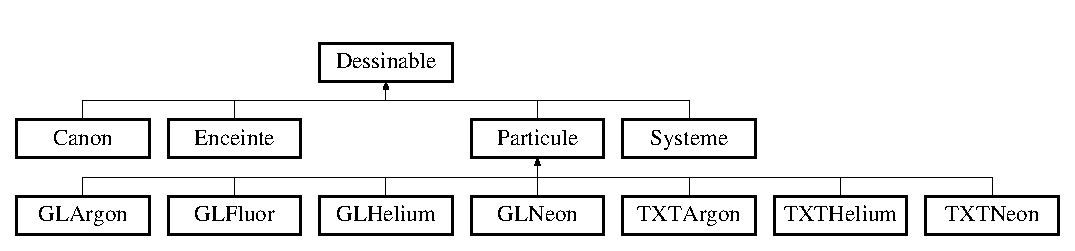
\includegraphics[height=2.926829cm]{class_dessinable}
\end{center}
\end{figure}
\subsection*{Fonctions membres publiques}
\begin{DoxyCompactItemize}
\item 
virtual void {\bf dessine} () const =0
\begin{DoxyCompactList}\small\item\em une méthode virtuelle pure car on veut qu'elle soit redéfinie dans toutes les sous-\/classes \end{DoxyCompactList}\end{DoxyCompactItemize}


\subsection{Description détaillée}


Définition à la ligne {\bf 12} du fichier {\bf Dessinable.\+h}.



\subsection{Documentation des fonctions membres}
\index{Dessinable@{Dessinable}!dessine@{dessine}}
\index{dessine@{dessine}!Dessinable@{Dessinable}}
\subsubsection[{dessine}]{\setlength{\rightskip}{0pt plus 5cm}virtual void Dessinable\+::dessine (
\begin{DoxyParamCaption}
{}
\end{DoxyParamCaption}
) const\hspace{0.3cm}{\ttfamily [pure virtual]}}\label{class_dessinable_aea37dacb2b67d6650a435d72c9a6fe79}


une méthode virtuelle pure car on veut qu'elle soit redéfinie dans toutes les sous-\/classes 



Implémenté dans {\bf Systeme} \doxyref{}{p.}{class_systeme_abc34a6c64e42d303be77d5df97ff377f}, {\bf Canon} \doxyref{}{p.}{class_canon_a2b43d0c2037d44c89b4c6d57b2f00fc1}, {\bf Enceinte} \doxyref{}{p.}{class_enceinte_aa2cdbb9cd5acf1a8593bc182f5ced6d1}, {\bf G\+L\+Fluor} \doxyref{}{p.}{class_g_l_fluor_ab4b02adef320b55887fea80a70c53131}, {\bf G\+L\+Argon} \doxyref{}{p.}{class_g_l_argon_af46a155b29b7149c89db2b6b909f3269}, {\bf G\+L\+Neon} \doxyref{}{p.}{class_g_l_neon_a9829245529338e0f9f20395bf769f9de}, {\bf G\+L\+Helium} \doxyref{}{p.}{class_g_l_helium_a425b1c773fa42f6e244d4036cbcb6ea3}, {\bf T\+X\+T\+Argon} \doxyref{}{p.}{class_t_x_t_argon_a5ce4904e93016605cb09a9772d856b57}, {\bf T\+X\+T\+Helium} \doxyref{}{p.}{class_t_x_t_helium_a4125af216d86b3015defe5a7126d18dd}, et {\bf T\+X\+T\+Neon} \doxyref{}{p.}{class_t_x_t_neon_a11437f76119ab389a3e47237be3a5571}.



La documentation de cette classe a été générée à partir du fichier suivant \+:\begin{DoxyCompactItemize}
\item 
/\+Users/burkhard/\+Dropbox/projet d'info/maximilian-\/g065/\+Simulation d'un gaz parfait/{\bf Dessinable.\+h}\end{DoxyCompactItemize}

\section{Référence de la classe Enceinte}
\label{class_enceinte}\index{Enceinte@{Enceinte}}


{\ttfamily \#include $<$Enceinte.\+h$>$}

Graphe d'héritage de Enceinte\+:\begin{figure}[H]
\begin{center}
\leavevmode
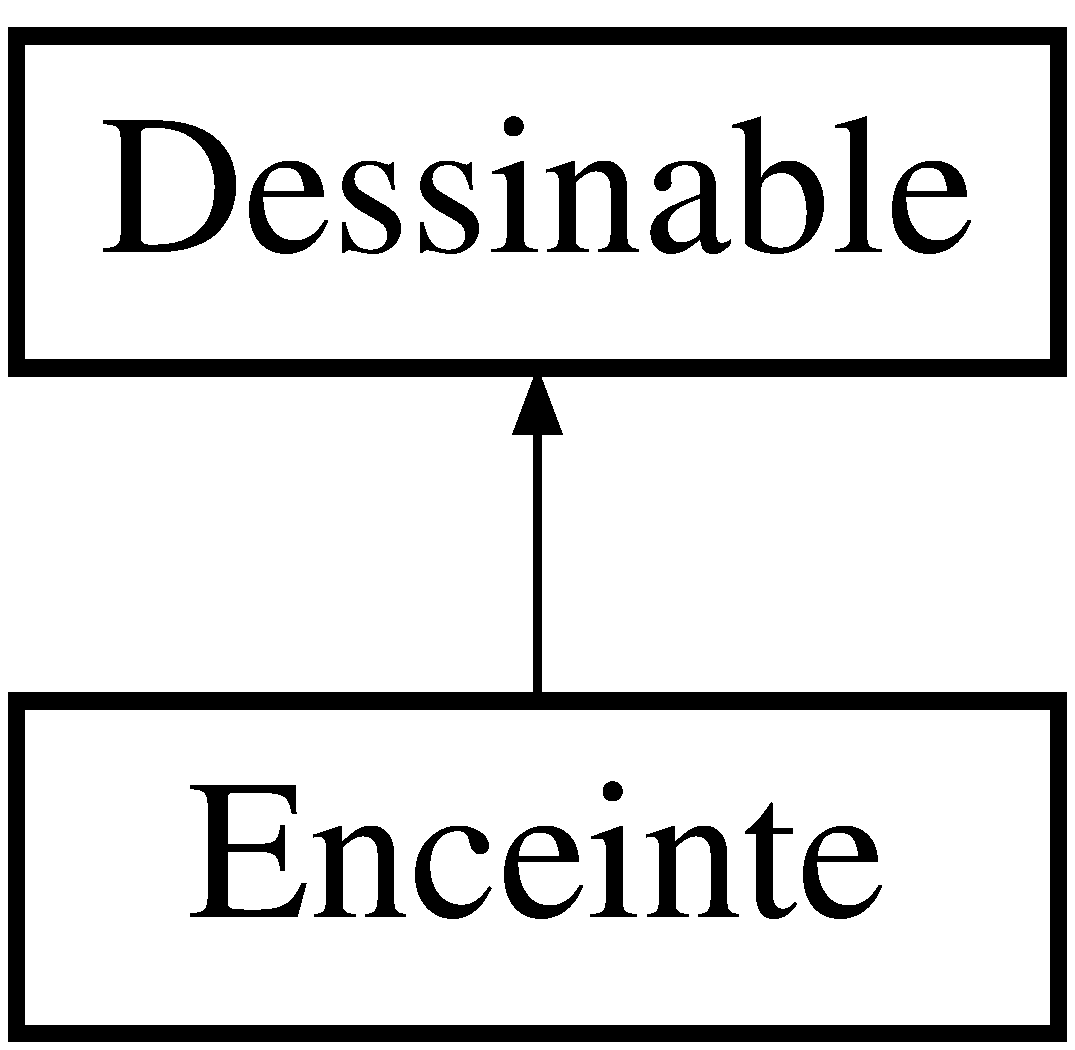
\includegraphics[height=2.000000cm]{class_enceinte}
\end{center}
\end{figure}
\subsection*{Fonctions membres publiques}
\begin{DoxyCompactItemize}
\item 
{\bf Enceinte} ()
\begin{DoxyCompactList}\small\item\em Constructeur sans paramètre. \end{DoxyCompactList}\item 
{\bf Enceinte} (bool reglage)
\begin{DoxyCompactList}\small\item\em Constructeur avec paramètre bool pour l'interface utilisateur. \end{DoxyCompactList}\item 
{\bf Enceinte} (double largeur, double longueur, double hauteur)
\begin{DoxyCompactList}\small\item\em Constructeur avec paramètres largeur, longueur et hauteur de l'enceinte. \end{DoxyCompactList}\item 
double {\bf get\+Largeur} () const 
\begin{DoxyCompactList}\small\item\em Prototype du getters de la largeur de l'enceinte. \end{DoxyCompactList}\item 
double {\bf get\+Longueur} () const 
\begin{DoxyCompactList}\small\item\em Prototype du getters de la longueur de l'enceinte. \end{DoxyCompactList}\item 
double {\bf get\+Hauteur} () const 
\begin{DoxyCompactList}\small\item\em Prototype du getters de la hauteur de l'enceinte. \end{DoxyCompactList}\item 
void {\bf display} () const 
\begin{DoxyCompactList}\small\item\em Prototype de la méthode qui écrit dans le terminal la largeur hauteur et longueur de l'enceinte. \end{DoxyCompactList}\item 
virtual void {\bf dessine} () const 
\begin{DoxyCompactList}\small\item\em Prototype de la méthode dessine en Open\+G\+L. \end{DoxyCompactList}\end{DoxyCompactItemize}


\subsection{Description détaillée}
Cette classe est celle qui permet de créer une enceinte, de la dessiner graĉe au fait qu'elle hérite de dessinable donc nous avons pu utiliser le polymophisme pour appeler la méthode dessine. 

Définition à la ligne {\bf 19} du fichier {\bf Enceinte.\+h}.



\subsection{Documentation des constructeurs et destructeur}
\index{Enceinte@{Enceinte}!Enceinte@{Enceinte}}
\index{Enceinte@{Enceinte}!Enceinte@{Enceinte}}
\subsubsection[{Enceinte}]{\setlength{\rightskip}{0pt plus 5cm}Enceinte\+::\+Enceinte (
\begin{DoxyParamCaption}
{}
\end{DoxyParamCaption}
)}\label{class_enceinte_abe74eac05c7cacb5ad09c0e99c4301a4}


Constructeur sans paramètre. 

Constructeur de la classe de l'enceinte mais qui initialise à largeur = 100, longueur =100, hauteur = 100 

Définition à la ligne {\bf 27} du fichier {\bf Enceinte.\+cc}.

\index{Enceinte@{Enceinte}!Enceinte@{Enceinte}}
\index{Enceinte@{Enceinte}!Enceinte@{Enceinte}}
\subsubsection[{Enceinte}]{\setlength{\rightskip}{0pt plus 5cm}Enceinte\+::\+Enceinte (
\begin{DoxyParamCaption}
\item[{bool}]{reglage}
\end{DoxyParamCaption}
)}\label{class_enceinte_ac535eaee140265078b89a559d08edc90}


Constructeur avec paramètre bool pour l'interface utilisateur. 

Constructeur de la classe de l'enceinte mais qui initialise aux valeurs prises comme paramètre


\begin{DoxyParams}{Paramètres}
{\em bool} & reglage \+: permet en fonction de l'utilisateur souhaite d'avoir un appel différents du constructeur \\
\hline
\end{DoxyParams}


Définition à la ligne {\bf 38} du fichier {\bf Enceinte.\+cc}.

\index{Enceinte@{Enceinte}!Enceinte@{Enceinte}}
\index{Enceinte@{Enceinte}!Enceinte@{Enceinte}}
\subsubsection[{Enceinte}]{\setlength{\rightskip}{0pt plus 5cm}Enceinte\+::\+Enceinte (
\begin{DoxyParamCaption}
\item[{double}]{largeur, }
\item[{double}]{longueur, }
\item[{double}]{hauteur}
\end{DoxyParamCaption}
)}\label{class_enceinte_a2fb9ccf810a5fbfd846913c597335928}


Constructeur avec paramètres largeur, longueur et hauteur de l'enceinte. 

Constructeur de la classe de l'enceinte mais qui initialise aux valeurs prises comme paramètre


\begin{DoxyParams}{Paramètres}
{\em double} & largeur \\
\hline
{\em double} & longueur \\
\hline
{\em double} & hauteur \\
\hline
\end{DoxyParams}


Définition à la ligne {\bf 64} du fichier {\bf Enceinte.\+cc}.



\subsection{Documentation des fonctions membres}
\index{Enceinte@{Enceinte}!dessine@{dessine}}
\index{dessine@{dessine}!Enceinte@{Enceinte}}
\subsubsection[{dessine}]{\setlength{\rightskip}{0pt plus 5cm}void Enceinte\+::dessine (
\begin{DoxyParamCaption}
{}
\end{DoxyParamCaption}
) const\hspace{0.3cm}{\ttfamily [virtual]}}\label{class_enceinte_aa2cdbb9cd5acf1a8593bc182f5ced6d1}


Prototype de la méthode dessine en Open\+G\+L. 

définition de la méthode dessine de l'enceinte en Open\+G\+L

elle va prendre prendre une couleur noire, et dessiner des traits qui vont faire le tours de l'enceinte 

Implémente {\bf Dessinable} \doxyref{}{p.}{class_dessinable_aea37dacb2b67d6650a435d72c9a6fe79}.



Définition à la ligne {\bf 113} du fichier {\bf Enceinte.\+cc}.

\index{Enceinte@{Enceinte}!display@{display}}
\index{display@{display}!Enceinte@{Enceinte}}
\subsubsection[{display}]{\setlength{\rightskip}{0pt plus 5cm}void Enceinte\+::display (
\begin{DoxyParamCaption}
{}
\end{DoxyParamCaption}
) const}\label{class_enceinte_ad2ae6703d36a71931c5cf05f9e72bbe7}


Prototype de la méthode qui écrit dans le terminal la largeur hauteur et longueur de l'enceinte. 

méthode pour afficher dans le terminal la dimension de l'enceinte 

Définition à la ligne {\bf 101} du fichier {\bf Enceinte.\+cc}.

\index{Enceinte@{Enceinte}!get\+Hauteur@{get\+Hauteur}}
\index{get\+Hauteur@{get\+Hauteur}!Enceinte@{Enceinte}}
\subsubsection[{get\+Hauteur}]{\setlength{\rightskip}{0pt plus 5cm}double Enceinte\+::get\+Hauteur (
\begin{DoxyParamCaption}
{}
\end{DoxyParamCaption}
) const}\label{class_enceinte_a313cc6bc2baf718a99cf0b10bb9e7f51}


Prototype du getters de la hauteur de l'enceinte. 

Methode qui permet de retourner les attributs privés de la hauteur

\begin{DoxyReturn}{Renvoie}
la hauteur 
\end{DoxyReturn}


Définition à la ligne {\bf 94} du fichier {\bf Enceinte.\+cc}.

\index{Enceinte@{Enceinte}!get\+Largeur@{get\+Largeur}}
\index{get\+Largeur@{get\+Largeur}!Enceinte@{Enceinte}}
\subsubsection[{get\+Largeur}]{\setlength{\rightskip}{0pt plus 5cm}double Enceinte\+::get\+Largeur (
\begin{DoxyParamCaption}
{}
\end{DoxyParamCaption}
) const}\label{class_enceinte_a553db9446669114f47a28e59ebbd4064}


Prototype du getters de la largeur de l'enceinte. 

Methode qui permet de retourner les attributs privés de la largeur

\begin{DoxyReturn}{Renvoie}
la largeur 
\end{DoxyReturn}


Définition à la ligne {\bf 76} du fichier {\bf Enceinte.\+cc}.

\index{Enceinte@{Enceinte}!get\+Longueur@{get\+Longueur}}
\index{get\+Longueur@{get\+Longueur}!Enceinte@{Enceinte}}
\subsubsection[{get\+Longueur}]{\setlength{\rightskip}{0pt plus 5cm}double Enceinte\+::get\+Longueur (
\begin{DoxyParamCaption}
{}
\end{DoxyParamCaption}
) const}\label{class_enceinte_ab5a4c9f43bc1640f14e0e960e8fe76b9}


Prototype du getters de la longueur de l'enceinte. 

Methode qui permet de retourner les attributs privés de la longueur

\begin{DoxyReturn}{Renvoie}
la longueur 
\end{DoxyReturn}


Définition à la ligne {\bf 85} du fichier {\bf Enceinte.\+cc}.



La documentation de cette classe a été générée à partir des fichiers suivants \+:\begin{DoxyCompactItemize}
\item 
/\+Users/burkhard/\+Dropbox/projet d'info/maximilian-\/g065/\+Simulation d'un gaz parfait/{\bf Enceinte.\+h}\item 
/\+Users/burkhard/\+Dropbox/projet d'info/maximilian-\/g065/\+Simulation d'un gaz parfait/{\bf Enceinte.\+cc}\end{DoxyCompactItemize}

\section{Référence de la classe Fenetre}
\label{class_fenetre}\index{Fenetre@{Fenetre}}


{\ttfamily \#include $<$Fenetre.\+h$>$}

Graphe d'héritage de Fenetre\+:\begin{figure}[H]
\begin{center}
\leavevmode
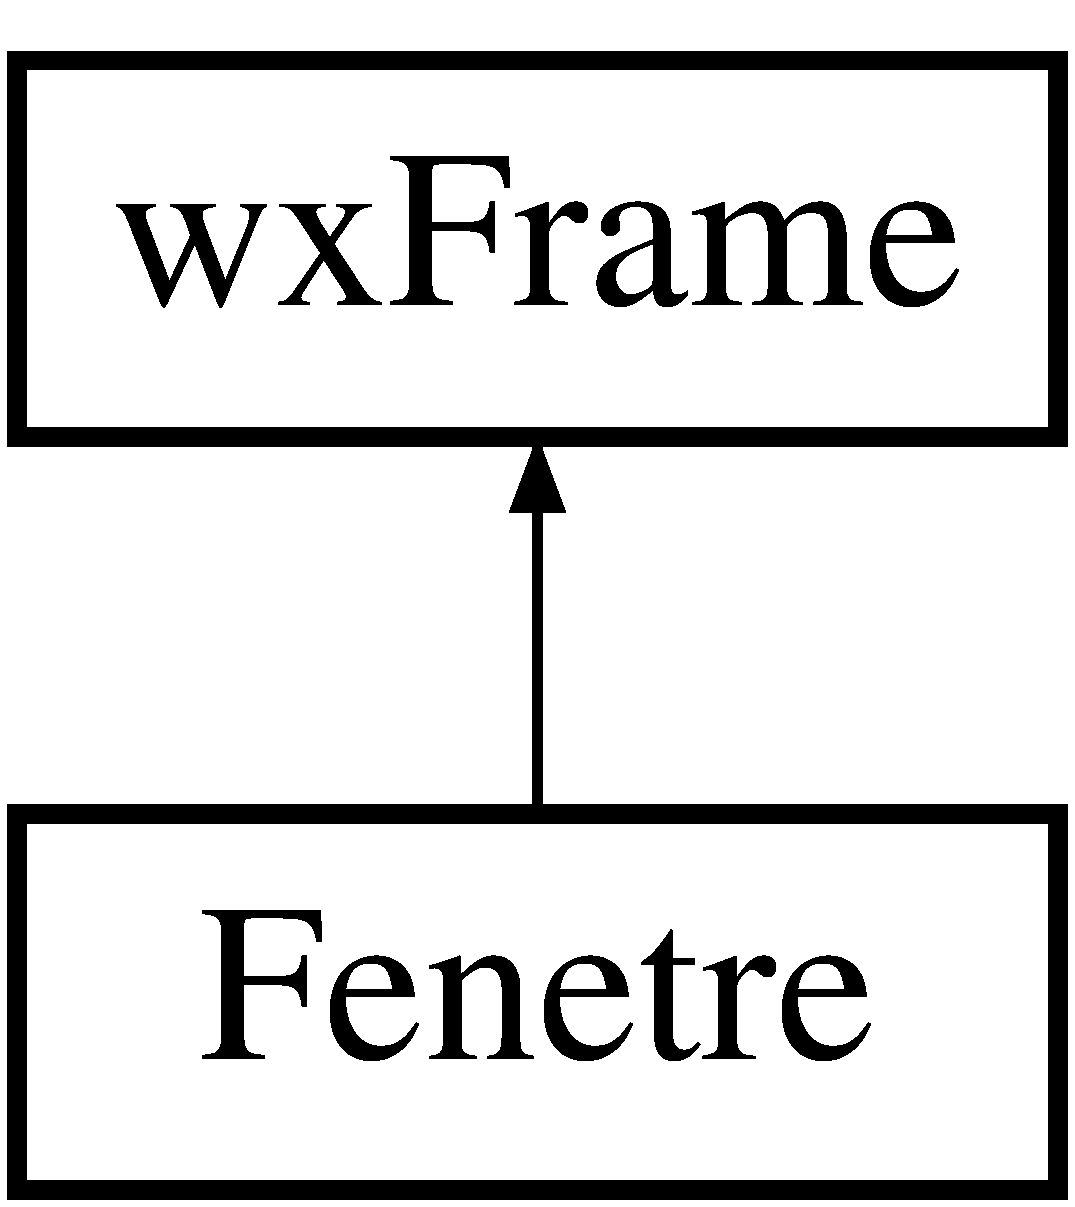
\includegraphics[height=2.000000cm]{class_fenetre}
\end{center}
\end{figure}
\subsection*{Fonctions membres publiques}
\begin{DoxyCompactItemize}
\item 
{\bf Fenetre} (wx\+String const \&titre, wx\+Size const \&taille=wx\+Default\+Size, wx\+Point const \&position=wx\+Default\+Position, long style=wx\+D\+E\+F\+A\+U\+L\+T\+\_\+\+F\+R\+A\+M\+E\+\_\+\+S\+T\+Y\+L\+E)
\begin{DoxyCompactList}\small\item\em Constructeur avec arguments. \end{DoxyCompactList}\item 
{\bf Fenetre} (wx\+String const \&titre, bool reglage, wx\+Size const \&taille=wx\+Default\+Size, wx\+Point const \&position=wx\+Default\+Position, long style=wx\+D\+E\+F\+A\+U\+L\+T\+\_\+\+F\+R\+A\+M\+E\+\_\+\+S\+T\+Y\+L\+E)
\begin{DoxyCompactList}\small\item\em Constructeur avec arguments et reglage pour l'interface utilisateur. \end{DoxyCompactList}\item 
virtual {\bf $\sim$\+Fenetre} ()
\begin{DoxyCompactList}\small\item\em destructeur de fenetre \end{DoxyCompactList}\end{DoxyCompactItemize}
\subsection*{Fonctions membres protégées}
\begin{DoxyCompactItemize}
\item 
void {\bf On\+Exit} (wx\+Command\+Event \&event)
\begin{DoxyCompactList}\small\item\em méthode pour pouvoir refermer la fenetre \end{DoxyCompactList}\end{DoxyCompactItemize}
\subsection*{Attributs protégés}
\begin{DoxyCompactItemize}
\item 
{\bf Vue\+\_\+\+Open\+G\+L} $\ast$ {\bf fogl}
\end{DoxyCompactItemize}


\subsection{Description détaillée}
Prototype de la classe \doxyref{Fenetre}{p.}{class_fenetre} pour l'Open\+G\+L et permet de créer une fenetre avec les caractéristiques que l'on souhaite. 

Définition à la ligne {\bf 23} du fichier {\bf Fenetre.\+h}.



\subsection{Documentation des constructeurs et destructeur}
\index{Fenetre@{Fenetre}!Fenetre@{Fenetre}}
\index{Fenetre@{Fenetre}!Fenetre@{Fenetre}}
\subsubsection[{Fenetre}]{\setlength{\rightskip}{0pt plus 5cm}Fenetre\+::\+Fenetre (
\begin{DoxyParamCaption}
\item[{wx\+String const \&}]{titre, }
\item[{wx\+Size const \&}]{taille = {\ttfamily wxDefaultSize}, }
\item[{wx\+Point const \&}]{position = {\ttfamily wxDefaultPosition}, }
\item[{long}]{style = {\ttfamily wxDEFAULT\+\_\+FRAME\+\_\+STYLE}}
\end{DoxyParamCaption}
)}\label{class_fenetre_a3b78862724264ec79d0332f8f65632aa}


Constructeur avec arguments. 

Constructeur de la classe \doxyref{Vecteur}{p.}{class_vecteur} avec trois arguements de type double \begin{DoxyVerb}\param titre : le nom que portera la fenetre
\param taille : donne la taille de la fenetre
\param position : place la fenetre à l'endroit voulu
\param style : style de la fenêtre\end{DoxyVerb}
 Barre de menu

Barre de menu

Barre de menu

Barre de menu

Affiche (montre) la fenetre

Initialise Open\+G\+L 

Définition à la ligne {\bf 28} du fichier {\bf Fenetre.\+cc}.

\index{Fenetre@{Fenetre}!Fenetre@{Fenetre}}
\index{Fenetre@{Fenetre}!Fenetre@{Fenetre}}
\subsubsection[{Fenetre}]{\setlength{\rightskip}{0pt plus 5cm}Fenetre\+::\+Fenetre (
\begin{DoxyParamCaption}
\item[{wx\+String const \&}]{titre, }
\item[{bool}]{reglage, }
\item[{wx\+Size const \&}]{taille = {\ttfamily wxDefaultSize}, }
\item[{wx\+Point const \&}]{position = {\ttfamily wxDefaultPosition}, }
\item[{long}]{style = {\ttfamily wxDEFAULT\+\_\+FRAME\+\_\+STYLE}}
\end{DoxyParamCaption}
)}\label{class_fenetre_a0c4225ac5a9b265b860a610204a37024}


Constructeur avec arguments et reglage pour l'interface utilisateur. 

Constructeur de la classe, permet de gérer l'interface utilisateur Nous avons décider de le faire comem cela car ça nous permettait de le faire simplement en respectant une meilleure conception


\begin{DoxyParams}{Paramètres}
{\em titre} & \+: le nom que portera la fenetre \\
\hline
{\em reglage} & \+: permet de gérer les souahaits de l'utilisateur \\
\hline
{\em taille} & \+: donne la taille de la fenetre \\
\hline
{\em position} & \+: place la fenetre à l'endroit voulu \\
\hline
{\em style} & \+: style de la fenêtre \\
\hline
\end{DoxyParams}
Barre de menu

Barre de menu

Barre de menu

Barre de menu

Affiche (montre) la fenetre

Initialise Open\+G\+L 

Définition à la ligne {\bf 65} du fichier {\bf Fenetre.\+cc}.

\index{Fenetre@{Fenetre}!````~Fenetre@{$\sim$\+Fenetre}}
\index{````~Fenetre@{$\sim$\+Fenetre}!Fenetre@{Fenetre}}
\subsubsection[{$\sim$\+Fenetre}]{\setlength{\rightskip}{0pt plus 5cm}virtual Fenetre\+::$\sim$\+Fenetre (
\begin{DoxyParamCaption}
{}
\end{DoxyParamCaption}
)\hspace{0.3cm}{\ttfamily [inline]}, {\ttfamily [virtual]}}\label{class_fenetre_a74e5aa1f39a581ae746f3832200fd055}


destructeur de fenetre 



Définition à la ligne {\bf 42} du fichier {\bf Fenetre.\+h}.



\subsection{Documentation des fonctions membres}
\index{Fenetre@{Fenetre}!On\+Exit@{On\+Exit}}
\index{On\+Exit@{On\+Exit}!Fenetre@{Fenetre}}
\subsubsection[{On\+Exit}]{\setlength{\rightskip}{0pt plus 5cm}void Fenetre\+::\+On\+Exit (
\begin{DoxyParamCaption}
\item[{wx\+Command\+Event \&}]{event}
\end{DoxyParamCaption}
)\hspace{0.3cm}{\ttfamily [inline]}, {\ttfamily [protected]}}\label{class_fenetre_a7d11a13eb53924e62623a4c80f51d431}


méthode pour pouvoir refermer la fenetre 



Définition à la ligne {\bf 46} du fichier {\bf Fenetre.\+h}.



\subsection{Documentation des données membres}
\index{Fenetre@{Fenetre}!fogl@{fogl}}
\index{fogl@{fogl}!Fenetre@{Fenetre}}
\subsubsection[{fogl}]{\setlength{\rightskip}{0pt plus 5cm}{\bf Vue\+\_\+\+Open\+G\+L}$\ast$ Fenetre\+::fogl\hspace{0.3cm}{\ttfamily [protected]}}\label{class_fenetre_aff0b26df4f97c060347155fec97223fe}


Définition à la ligne {\bf 49} du fichier {\bf Fenetre.\+h}.



La documentation de cette classe a été générée à partir des fichiers suivants \+:\begin{DoxyCompactItemize}
\item 
/\+Users/burkhard/\+Dropbox/projet d'info/maximilian-\/g065/\+Simulation d'un gaz parfait/{\bf Fenetre.\+h}\item 
/\+Users/burkhard/\+Dropbox/projet d'info/maximilian-\/g065/\+Simulation d'un gaz parfait/{\bf Fenetre.\+cc}\end{DoxyCompactItemize}

\section{Référence de la classe Generateur\+Aleatoire}
\label{class_generateur_aleatoire}\index{Generateur\+Aleatoire@{Generateur\+Aleatoire}}


Représente des objets capables de générer des nombres aléatoires.  




{\ttfamily \#include $<$Generateur\+Aleatoire.\+h$>$}

\subsection*{Fonctions membres publiques}
\begin{DoxyCompactItemize}
\item 
{\bf Generateur\+Aleatoire} ()
\begin{DoxyCompactList}\small\item\em Constructeur par défaut. \end{DoxyCompactList}\item 
{\bf Generateur\+Aleatoire} (unsigned int graine)
\begin{DoxyCompactList}\small\item\em Constructeur. \end{DoxyCompactList}\item 
int {\bf uniforme\+\_\+entier} (int min, int max)
\begin{DoxyCompactList}\small\item\em Méthode permettant de tirer uniformément un entier sur l'intervalle [min, max]. \end{DoxyCompactList}\item 
double {\bf uniforme\+\_\+reel} (double min, double max)
\begin{DoxyCompactList}\small\item\em Méthode permettant de tirer uniformément un réel sur l'intervalle [min, max[. \end{DoxyCompactList}\item 
double {\bf gaussienne} (double moyenne, double ecart\+\_\+type)
\begin{DoxyCompactList}\small\item\em Méthode permettant de tirer un réel suivant la loi normale des probablités (dîtes loi de Gauss) \end{DoxyCompactList}\end{DoxyCompactItemize}


\subsection{Description détaillée}
Représente des objets capables de générer des nombres aléatoires. 

Plusieurs méthodes peuvent être utilisées pour réaliser différents types de tirage 

Définition à la ligne {\bf 20} du fichier {\bf Generateur\+Aleatoire.\+h}.



\subsection{Documentation des constructeurs et destructeur}
\index{Generateur\+Aleatoire@{Generateur\+Aleatoire}!Generateur\+Aleatoire@{Generateur\+Aleatoire}}
\index{Generateur\+Aleatoire@{Generateur\+Aleatoire}!Generateur\+Aleatoire@{Generateur\+Aleatoire}}
\subsubsection[{Generateur\+Aleatoire}]{\setlength{\rightskip}{0pt plus 5cm}Generateur\+Aleatoire\+::\+Generateur\+Aleatoire (
\begin{DoxyParamCaption}
{}
\end{DoxyParamCaption}
)}\label{class_generateur_aleatoire_ac816c2c7554428f5f6c1af497e788a96}


Constructeur par défaut. 

Constructeur sans paramètre. Permet d'initialiser l'attribut générateur avec un nombre aléatoire 

Définition à la ligne {\bf 16} du fichier {\bf Generateur\+Aleatoire.\+cc}.

\index{Generateur\+Aleatoire@{Generateur\+Aleatoire}!Generateur\+Aleatoire@{Generateur\+Aleatoire}}
\index{Generateur\+Aleatoire@{Generateur\+Aleatoire}!Generateur\+Aleatoire@{Generateur\+Aleatoire}}
\subsubsection[{Generateur\+Aleatoire}]{\setlength{\rightskip}{0pt plus 5cm}Generateur\+Aleatoire\+::\+Generateur\+Aleatoire (
\begin{DoxyParamCaption}
\item[{unsigned int}]{graine}
\end{DoxyParamCaption}
)}\label{class_generateur_aleatoire_a0bcc05dfe4e809c0bf9f4aff45d5dafa}


Constructeur. 

Constructeur prenant un paramètre de type int. Permet d'initialiser l'attribut générateur avec un nombre donné (utile pour debugger) 

Définition à la ligne {\bf 23} du fichier {\bf Generateur\+Aleatoire.\+cc}.



\subsection{Documentation des fonctions membres}
\index{Generateur\+Aleatoire@{Generateur\+Aleatoire}!gaussienne@{gaussienne}}
\index{gaussienne@{gaussienne}!Generateur\+Aleatoire@{Generateur\+Aleatoire}}
\subsubsection[{gaussienne}]{\setlength{\rightskip}{0pt plus 5cm}double Generateur\+Aleatoire\+::gaussienne (
\begin{DoxyParamCaption}
\item[{double}]{moyenne, }
\item[{double}]{ecart\+\_\+type}
\end{DoxyParamCaption}
)}\label{class_generateur_aleatoire_af6a12956bb6af401e9f2d850b52a2b14}


Méthode permettant de tirer un réel suivant la loi normale des probablités (dîtes loi de Gauss) 


\begin{DoxyParams}{Paramètres}
{\em moyenne} & valeur autour de laquelle s'effectue le tirage \\
\hline
{\em ecart\+\_\+type} & valeur représentant l'écart moyen à la moyenne des valeurs du tirage\\
\hline
\end{DoxyParams}
\begin{DoxyReturn}{Renvoie}
Retourne un réel tiré selon la loi normale N(moyenne, ecart\+\_\+type) 
\end{DoxyReturn}


Définition à la ligne {\bf 50} du fichier {\bf Generateur\+Aleatoire.\+cc}.

\index{Generateur\+Aleatoire@{Generateur\+Aleatoire}!uniforme\+\_\+entier@{uniforme\+\_\+entier}}
\index{uniforme\+\_\+entier@{uniforme\+\_\+entier}!Generateur\+Aleatoire@{Generateur\+Aleatoire}}
\subsubsection[{uniforme\+\_\+entier}]{\setlength{\rightskip}{0pt plus 5cm}int Generateur\+Aleatoire\+::uniforme\+\_\+entier (
\begin{DoxyParamCaption}
\item[{int}]{min, }
\item[{int}]{max}
\end{DoxyParamCaption}
)}\label{class_generateur_aleatoire_a986164a020693bee0a8043fcd0c3953f}


Méthode permettant de tirer uniformément un entier sur l'intervalle [min, max]. 


\begin{DoxyParams}{Paramètres}
{\em min} & minimum de l'intervalle sur lequel le tirage s'effectue \\
\hline
{\em max} & maximum de l'intervalle sur lequel le tirage s'effectue\\
\hline
\end{DoxyParams}
\begin{DoxyReturn}{Renvoie}
Retourne un entier tiré uniformément sur [min, max] 
\end{DoxyReturn}


Définition à la ligne {\bf 32} du fichier {\bf Generateur\+Aleatoire.\+cc}.

\index{Generateur\+Aleatoire@{Generateur\+Aleatoire}!uniforme\+\_\+reel@{uniforme\+\_\+reel}}
\index{uniforme\+\_\+reel@{uniforme\+\_\+reel}!Generateur\+Aleatoire@{Generateur\+Aleatoire}}
\subsubsection[{uniforme\+\_\+reel}]{\setlength{\rightskip}{0pt plus 5cm}double Generateur\+Aleatoire\+::uniforme\+\_\+reel (
\begin{DoxyParamCaption}
\item[{double}]{min, }
\item[{double}]{max}
\end{DoxyParamCaption}
)}\label{class_generateur_aleatoire_a39d2eddd31748b5f35dfdc7bc7c7a7d2}


Méthode permettant de tirer uniformément un réel sur l'intervalle [min, max[. 


\begin{DoxyParams}{Paramètres}
{\em min} & minimum de l'intervalle sur lequel le tirage s'effectue \\
\hline
{\em max} & maximum de l'intervalle sur lequel le tirage s'effectue\\
\hline
\end{DoxyParams}
\begin{DoxyReturn}{Renvoie}
Retourne un réel tiré uniformément sur [min, max[ 
\end{DoxyReturn}


Définition à la ligne {\bf 41} du fichier {\bf Generateur\+Aleatoire.\+cc}.



La documentation de cette classe a été générée à partir des fichiers suivants \+:\begin{DoxyCompactItemize}
\item 
/\+Users/burkhard/\+Dropbox/projet d'info/maximilian-\/g065/\+Simulation d'un gaz parfait/{\bf Generateur\+Aleatoire.\+h}\item 
/\+Users/burkhard/\+Dropbox/projet d'info/maximilian-\/g065/\+Simulation d'un gaz parfait/{\bf Generateur\+Aleatoire.\+cc}\end{DoxyCompactItemize}

\section{Référence de la classe G\+L\+Argon}
\label{class_g_l_argon}\index{G\+L\+Argon@{G\+L\+Argon}}


Prototype de la classe \doxyref{G\+L\+Argon}{p.}{class_g_l_argon}.  




{\ttfamily \#include $<$G\+L\+Argon.\+h$>$}

Graphe d'héritage de G\+L\+Argon\+:\begin{figure}[H]
\begin{center}
\leavevmode
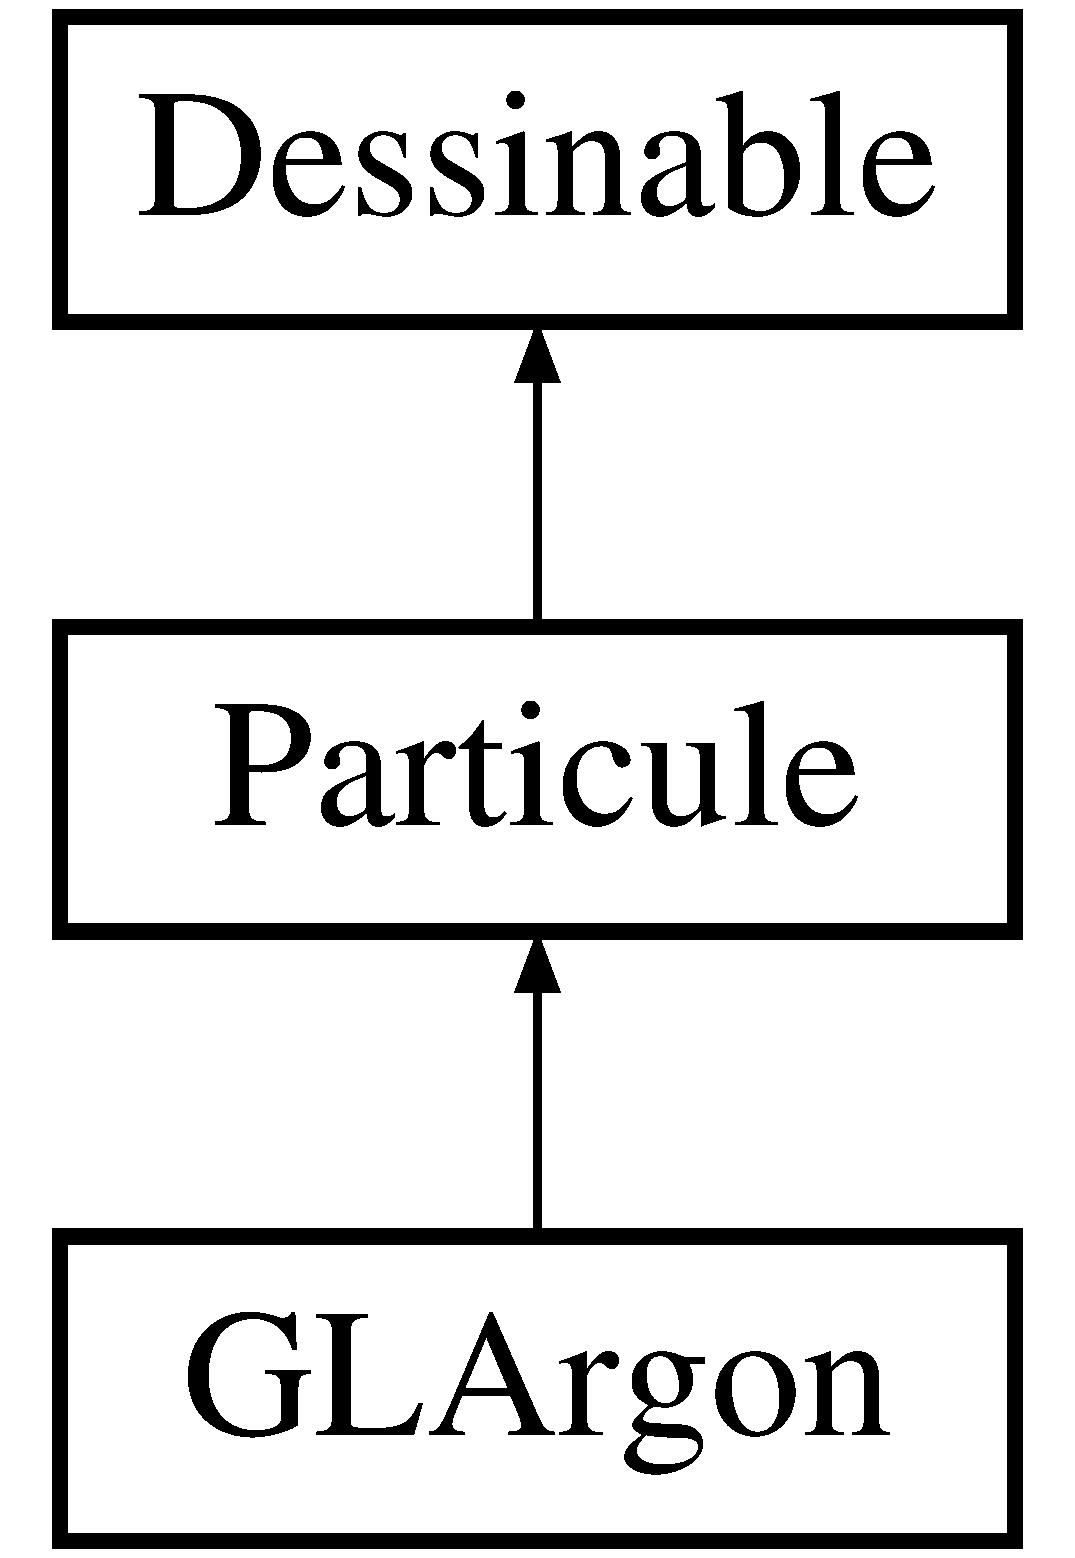
\includegraphics[height=3.000000cm]{class_g_l_argon}
\end{center}
\end{figure}
\subsection*{Fonctions membres publiques}
\begin{DoxyCompactItemize}
\item 
{\bf G\+L\+Argon} ({\bf Vecteur} {\bf position}, {\bf Vecteur} {\bf vitesse})
\begin{DoxyCompactList}\small\item\em Constructeur avec arguments sans la température du système. \end{DoxyCompactList}\item 
{\bf G\+L\+Argon} ({\bf Enceinte} const \&enceinte, {\bf Generateur\+Aleatoire} \&tirage, double temperature)
\begin{DoxyCompactList}\small\item\em Constructeur avec arguments avec la température du système et le tirage aléatoire des vecteurs positions. \end{DoxyCompactList}\item 
virtual {\bf $\sim$\+G\+L\+Argon} ()
\begin{DoxyCompactList}\small\item\em Dstructeurs. \end{DoxyCompactList}\item 
virtual void {\bf evolue} (double dt)
\begin{DoxyCompactList}\small\item\em Prototype de la méthode evolue. \end{DoxyCompactList}\item 
virtual void {\bf dessine} () const 
\begin{DoxyCompactList}\small\item\em Prototype de la méthode evolue. \end{DoxyCompactList}\end{DoxyCompactItemize}
\subsection*{Membres hérités additionnels}


\subsection{Description détaillée}
Prototype de la classe \doxyref{G\+L\+Argon}{p.}{class_g_l_argon}. 

Cette classe est celle qui permet de créer une particule d'argon en Open\+G\+L 

Définition à la ligne {\bf 25} du fichier {\bf G\+L\+Argon.\+h}.



\subsection{Documentation des constructeurs et destructeur}
\index{G\+L\+Argon@{G\+L\+Argon}!G\+L\+Argon@{G\+L\+Argon}}
\index{G\+L\+Argon@{G\+L\+Argon}!G\+L\+Argon@{G\+L\+Argon}}
\subsubsection[{G\+L\+Argon}]{\setlength{\rightskip}{0pt plus 5cm}G\+L\+Argon\+::\+G\+L\+Argon (
\begin{DoxyParamCaption}
\item[{{\bf Vecteur}}]{position, }
\item[{{\bf Vecteur}}]{vitesse}
\end{DoxyParamCaption}
)}\label{class_g_l_argon_a99e2ba6207d052993736dc5ec0176506}


Constructeur avec arguments sans la température du système. 

sans le paramètre de température, initialise un rayon et une masse à notre particule


\begin{DoxyParams}{Paramètres}
{\em position} & \+: est la position de la particule que l'on souhaite \\
\hline
{\em vitesse} & \+: est la vitesse de la particule que l'on souhaite \\
\hline
\end{DoxyParams}


Définition à la ligne {\bf 20} du fichier {\bf G\+L\+Argon.\+cc}.

\index{G\+L\+Argon@{G\+L\+Argon}!G\+L\+Argon@{G\+L\+Argon}}
\index{G\+L\+Argon@{G\+L\+Argon}!G\+L\+Argon@{G\+L\+Argon}}
\subsubsection[{G\+L\+Argon}]{\setlength{\rightskip}{0pt plus 5cm}G\+L\+Argon\+::\+G\+L\+Argon (
\begin{DoxyParamCaption}
\item[{{\bf Enceinte} const \&}]{enceinte, }
\item[{{\bf Generateur\+Aleatoire} \&}]{tirage, }
\item[{double}]{temperature}
\end{DoxyParamCaption}
)}\label{class_g_l_argon_af3fa2c1411ba06ea93b0922f4ca949c4}


Constructeur avec arguments avec la température du système et le tirage aléatoire des vecteurs positions. 

sans le paramètre de température, initialise un rayon et une masse à notre particule


\begin{DoxyParams}{Paramètres}
{\em enceinte} & \+: permet de connaitre les dimmensions de l'emceinte pour calculer les positions \\
\hline
{\em tirage} & \+: donne une position aléatoire de la particule dans l'enceinte \\
\hline
{\em gtempérature} & \+: la température que l'on souhaite pour calculer la vitesse \\
\hline
\end{DoxyParams}


Définition à la ligne {\bf 31} du fichier {\bf G\+L\+Argon.\+cc}.

\index{G\+L\+Argon@{G\+L\+Argon}!````~G\+L\+Argon@{$\sim$\+G\+L\+Argon}}
\index{````~G\+L\+Argon@{$\sim$\+G\+L\+Argon}!G\+L\+Argon@{G\+L\+Argon}}
\subsubsection[{$\sim$\+G\+L\+Argon}]{\setlength{\rightskip}{0pt plus 5cm}G\+L\+Argon\+::$\sim$\+G\+L\+Argon (
\begin{DoxyParamCaption}
{}
\end{DoxyParamCaption}
)\hspace{0.3cm}{\ttfamily [virtual]}}\label{class_g_l_argon_a4b63a77bed72014d211453e46de9a60c}


Dstructeurs. 



Définition à la ligne {\bf 35} du fichier {\bf G\+L\+Argon.\+cc}.



\subsection{Documentation des fonctions membres}
\index{G\+L\+Argon@{G\+L\+Argon}!dessine@{dessine}}
\index{dessine@{dessine}!G\+L\+Argon@{G\+L\+Argon}}
\subsubsection[{dessine}]{\setlength{\rightskip}{0pt plus 5cm}void G\+L\+Argon\+::dessine (
\begin{DoxyParamCaption}
{}
\end{DoxyParamCaption}
) const\hspace{0.3cm}{\ttfamily [virtual]}}\label{class_g_l_argon_af46a155b29b7149c89db2b6b909f3269}


Prototype de la méthode evolue. 

dessine la particule de couleur à la position souhaitée par une matrice de translation couleur vert, 100\% 

Implémente {\bf Dessinable} \doxyref{}{p.}{class_dessinable_aea37dacb2b67d6650a435d72c9a6fe79}.



Définition à la ligne {\bf 56} du fichier {\bf G\+L\+Argon.\+cc}.

\index{G\+L\+Argon@{G\+L\+Argon}!evolue@{evolue}}
\index{evolue@{evolue}!G\+L\+Argon@{G\+L\+Argon}}
\subsubsection[{evolue}]{\setlength{\rightskip}{0pt plus 5cm}void G\+L\+Argon\+::evolue (
\begin{DoxyParamCaption}
\item[{double}]{dt}
\end{DoxyParamCaption}
)\hspace{0.3cm}{\ttfamily [virtual]}}\label{class_g_l_argon_a18a22f3feb53956d69c52031d4f86b96}


Prototype de la méthode evolue. 

appelle la méthode évolue de la classe particule 
\begin{DoxyParams}{Paramètres}
{\em dt} & \+: le pas de temps \\
\hline
\end{DoxyParams}


Réimplémentée à partir de {\bf Particule} \doxyref{}{p.}{class_particule_a7c6a97e2b65d4326d36b6d3b6251b79c}.



Définition à la ligne {\bf 47} du fichier {\bf G\+L\+Argon.\+cc}.



La documentation de cette classe a été générée à partir des fichiers suivants \+:\begin{DoxyCompactItemize}
\item 
/\+Users/burkhard/\+Dropbox/projet d'info/maximilian-\/g065/\+Simulation d'un gaz parfait/{\bf G\+L\+Argon.\+h}\item 
/\+Users/burkhard/\+Dropbox/projet d'info/maximilian-\/g065/\+Simulation d'un gaz parfait/{\bf G\+L\+Argon.\+cc}\end{DoxyCompactItemize}

\section{Référence de la classe G\+L\+Fluor}
\label{class_g_l_fluor}\index{G\+L\+Fluor@{G\+L\+Fluor}}


Prototype de la classe G\+Lluor.  




{\ttfamily \#include $<$G\+L\+Fluor.\+h$>$}

Graphe d'héritage de G\+L\+Fluor\+:\begin{figure}[H]
\begin{center}
\leavevmode
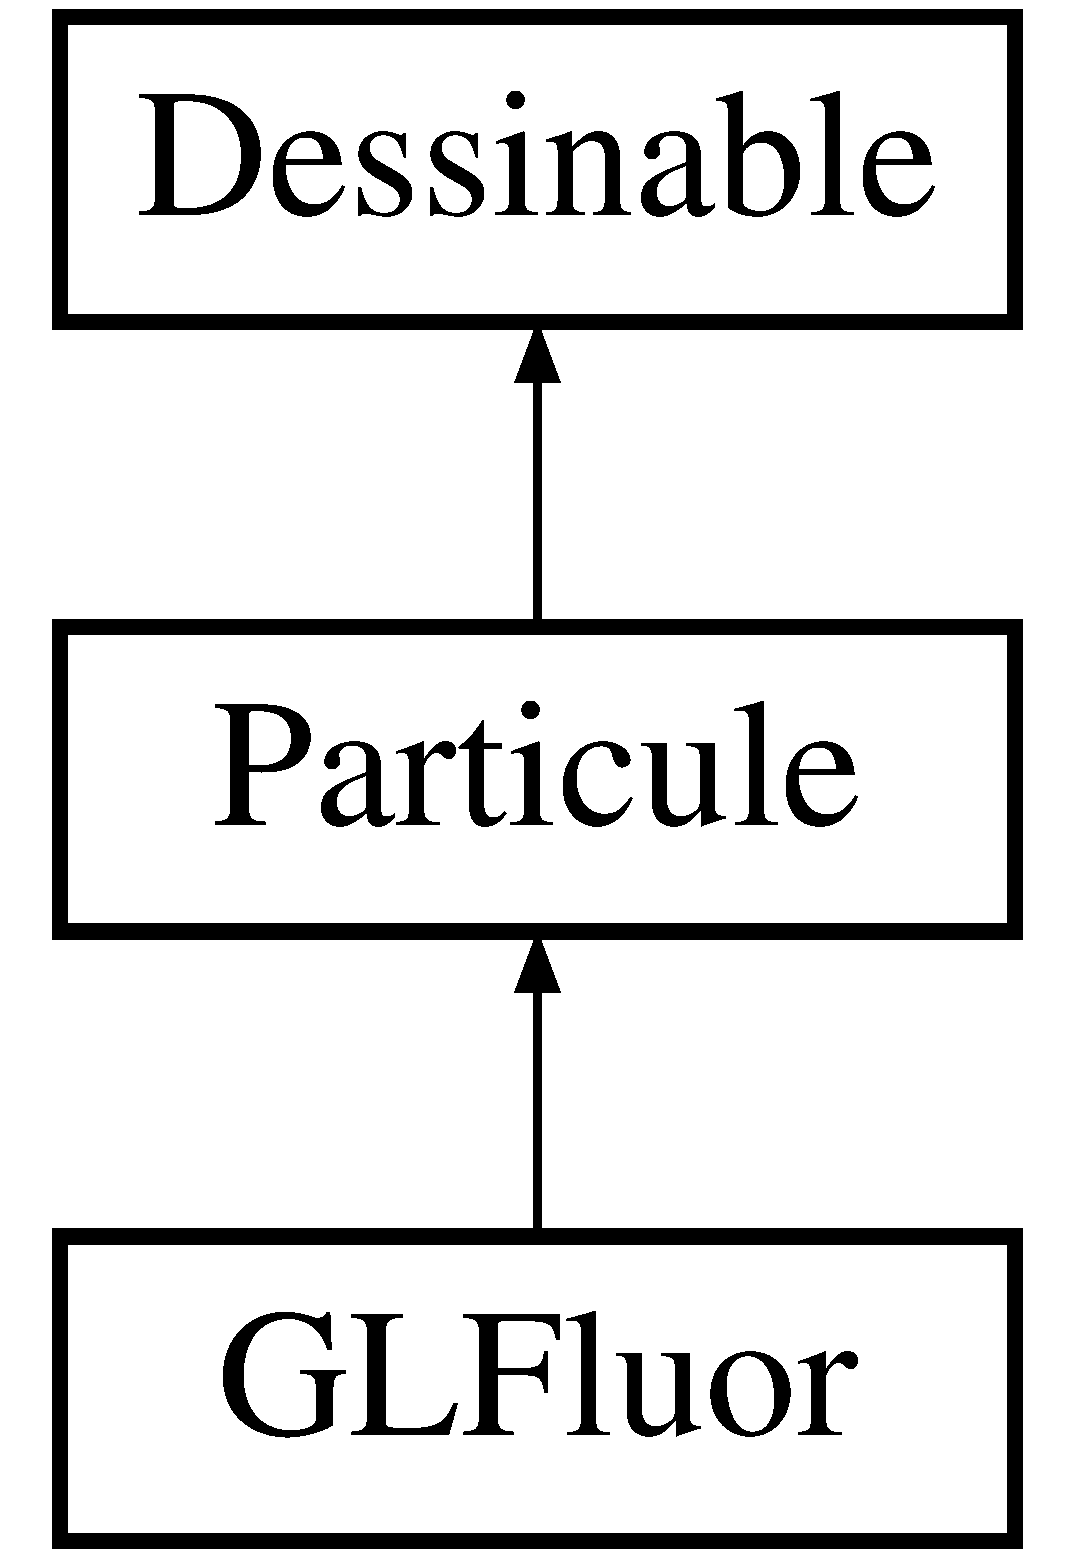
\includegraphics[height=3.000000cm]{class_g_l_fluor}
\end{center}
\end{figure}
\subsection*{Fonctions membres publiques}
\begin{DoxyCompactItemize}
\item 
{\bf G\+L\+Fluor} ({\bf Vecteur} {\bf position}, {\bf Vecteur} {\bf vitesse})
\begin{DoxyCompactList}\small\item\em Constructeur avec arguments sans la température du système. \end{DoxyCompactList}\item 
{\bf G\+L\+Fluor} ({\bf Enceinte} const \&enceinte, {\bf Generateur\+Aleatoire} \&tirage, double temperature)
\begin{DoxyCompactList}\small\item\em Constructeur avec arguments avec la température du système et le tirage aléatoire des vecteurs positions. \end{DoxyCompactList}\item 
virtual {\bf $\sim$\+G\+L\+Fluor} ()
\begin{DoxyCompactList}\small\item\em Dstructeurs. \end{DoxyCompactList}\item 
virtual void {\bf evolue} (double dt)
\begin{DoxyCompactList}\small\item\em Prototype de la méthode evolue. \end{DoxyCompactList}\item 
virtual void {\bf dessine} () const 
\begin{DoxyCompactList}\small\item\em Prototype de la méthode evolue. \end{DoxyCompactList}\item 
void {\bf enregistrer\+Coordonnee} ()
\begin{DoxyCompactList}\small\item\em Prototye de la méthode qui va enregistrer les coordonnées. \end{DoxyCompactList}\end{DoxyCompactItemize}
\subsection*{Membres hérités additionnels}


\subsection{Description détaillée}
Prototype de la classe G\+Lluor. 

Cette classe est celle qui permet de créer une particule de fluor en Open\+G\+L et permet aussi de suivre à la trace cette particule grâce à un deque qui enregistre chaque position pendant un certain intervalle. Nous avos pas besoins de toutes les positions d'ou le fait que nous supprimons après 150 pas de temps les anciennes positions. Nous avos choisis un deque car il fallait une faible complexité pour détruire la première ligne. 

Définition à la ligne {\bf 32} du fichier {\bf G\+L\+Fluor.\+h}.



\subsection{Documentation des constructeurs et destructeur}
\index{G\+L\+Fluor@{G\+L\+Fluor}!G\+L\+Fluor@{G\+L\+Fluor}}
\index{G\+L\+Fluor@{G\+L\+Fluor}!G\+L\+Fluor@{G\+L\+Fluor}}
\subsubsection[{G\+L\+Fluor}]{\setlength{\rightskip}{0pt plus 5cm}G\+L\+Fluor\+::\+G\+L\+Fluor (
\begin{DoxyParamCaption}
\item[{{\bf Vecteur}}]{position, }
\item[{{\bf Vecteur}}]{vitesse}
\end{DoxyParamCaption}
)}\label{class_g_l_fluor_acfc934283cbecc868492a28eadbd0390}


Constructeur avec arguments sans la température du système. 

Construteur.

sans le paramètre de température, initialise un rayon et une masse à notre particule


\begin{DoxyParams}{Paramètres}
{\em position} & \+: est la position de la particule que l'on souhaite \\
\hline
{\em vitesse} & \+: est la vitesse de la particule que l'on souhaite \\
\hline
\end{DoxyParams}


Définition à la ligne {\bf 22} du fichier {\bf G\+L\+Fluor.\+cc}.

\index{G\+L\+Fluor@{G\+L\+Fluor}!G\+L\+Fluor@{G\+L\+Fluor}}
\index{G\+L\+Fluor@{G\+L\+Fluor}!G\+L\+Fluor@{G\+L\+Fluor}}
\subsubsection[{G\+L\+Fluor}]{\setlength{\rightskip}{0pt plus 5cm}G\+L\+Fluor\+::\+G\+L\+Fluor (
\begin{DoxyParamCaption}
\item[{{\bf Enceinte} const \&}]{enceinte, }
\item[{{\bf Generateur\+Aleatoire} \&}]{tirage, }
\item[{double}]{temperature}
\end{DoxyParamCaption}
)}\label{class_g_l_fluor_a69e04138661d93c35dc7b5a69d794296}


Constructeur avec arguments avec la température du système et le tirage aléatoire des vecteurs positions. 

Construteur.

sans le paramètre de température, initialise un rayon et une masse à notre particule


\begin{DoxyParams}{Paramètres}
{\em enceinte} & \+: permet de connaitre les dimmensions de l'emceinte pour calculer les positions \\
\hline
{\em tirage} & \+: donne une position aléatoire de la particule dans l'enceinte \\
\hline
{\em gtempérature} & \+: la température que l'on souhaite pour calculer la vitesse \\
\hline
\end{DoxyParams}


Définition à la ligne {\bf 34} du fichier {\bf G\+L\+Fluor.\+cc}.

\index{G\+L\+Fluor@{G\+L\+Fluor}!````~G\+L\+Fluor@{$\sim$\+G\+L\+Fluor}}
\index{````~G\+L\+Fluor@{$\sim$\+G\+L\+Fluor}!G\+L\+Fluor@{G\+L\+Fluor}}
\subsubsection[{$\sim$\+G\+L\+Fluor}]{\setlength{\rightskip}{0pt plus 5cm}G\+L\+Fluor\+::$\sim$\+G\+L\+Fluor (
\begin{DoxyParamCaption}
{}
\end{DoxyParamCaption}
)\hspace{0.3cm}{\ttfamily [virtual]}}\label{class_g_l_fluor_a4b7eb611e78635965d15f058262f79de}


Dstructeurs. 



Définition à la ligne {\bf 38} du fichier {\bf G\+L\+Fluor.\+cc}.



\subsection{Documentation des fonctions membres}
\index{G\+L\+Fluor@{G\+L\+Fluor}!dessine@{dessine}}
\index{dessine@{dessine}!G\+L\+Fluor@{G\+L\+Fluor}}
\subsubsection[{dessine}]{\setlength{\rightskip}{0pt plus 5cm}void G\+L\+Fluor\+::dessine (
\begin{DoxyParamCaption}
{}
\end{DoxyParamCaption}
) const\hspace{0.3cm}{\ttfamily [virtual]}}\label{class_g_l_fluor_ab4b02adef320b55887fea80a70c53131}


Prototype de la méthode evolue. 

dessine les points contenu dans le tableau(deque)

dessine la particule de couleur à la position souhaitée par une matrice de translation permet de parcourir le tableau et de le dssiner

dessine les particlues

couleur mauve

J'ai remis 10 partout 

Implémente {\bf Dessinable} \doxyref{}{p.}{class_dessinable_aea37dacb2b67d6650a435d72c9a6fe79}.



Définition à la ligne {\bf 80} du fichier {\bf G\+L\+Fluor.\+cc}.

\index{G\+L\+Fluor@{G\+L\+Fluor}!enregistrer\+Coordonnee@{enregistrer\+Coordonnee}}
\index{enregistrer\+Coordonnee@{enregistrer\+Coordonnee}!G\+L\+Fluor@{G\+L\+Fluor}}
\subsubsection[{enregistrer\+Coordonnee}]{\setlength{\rightskip}{0pt plus 5cm}void G\+L\+Fluor\+::enregistrer\+Coordonnee (
\begin{DoxyParamCaption}
{}
\end{DoxyParamCaption}
)}\label{class_g_l_fluor_a1071ae99d4253fe736dc1f5bf3f4990d}


Prototye de la méthode qui va enregistrer les coordonnées. 

méthode qui enregistre la position/coordonnée de la particule et ensuite appelle la méthode évolue de la classe particule supprime la première valeur du tableau après 150 pas de temps (complexité de 1)

ajoute la dernière positions au deque 

Définition à la ligne {\bf 63} du fichier {\bf G\+L\+Fluor.\+cc}.

\index{G\+L\+Fluor@{G\+L\+Fluor}!evolue@{evolue}}
\index{evolue@{evolue}!G\+L\+Fluor@{G\+L\+Fluor}}
\subsubsection[{evolue}]{\setlength{\rightskip}{0pt plus 5cm}void G\+L\+Fluor\+::evolue (
\begin{DoxyParamCaption}
\item[{double}]{dt}
\end{DoxyParamCaption}
)\hspace{0.3cm}{\ttfamily [virtual]}}\label{class_g_l_fluor_a9fbbc20c3f158575d39fce6c9ca85931}


Prototype de la méthode evolue. 

spéciale pour le fluor car on enresitre ça position dans un deque (une sorte de tableau) pour pouvoir afficher la trajectoire Nous avons fait appel à evolue car c'est la seul méthode qui nous permettait d'enregistrer a tout instant


\begin{DoxyParams}{Paramètres}
{\em dt} & \+: le pas de temps \\
\hline
\end{DoxyParams}


Réimplémentée à partir de {\bf Particule} \doxyref{}{p.}{class_particule_a7c6a97e2b65d4326d36b6d3b6251b79c}.



Définition à la ligne {\bf 54} du fichier {\bf G\+L\+Fluor.\+cc}.



La documentation de cette classe a été générée à partir des fichiers suivants \+:\begin{DoxyCompactItemize}
\item 
/\+Users/burkhard/\+Dropbox/projet d'info/maximilian-\/g065/\+Simulation d'un gaz parfait/{\bf G\+L\+Fluor.\+h}\item 
/\+Users/burkhard/\+Dropbox/projet d'info/maximilian-\/g065/\+Simulation d'un gaz parfait/{\bf G\+L\+Fluor.\+cc}\end{DoxyCompactItemize}

\section{Référence de la classe G\+L\+Helium}
\label{class_g_l_helium}\index{G\+L\+Helium@{G\+L\+Helium}}


Prototype de la classe \doxyref{G\+L\+Helium}{p.}{class_g_l_helium}.  




{\ttfamily \#include $<$G\+L\+Helium.\+h$>$}

Graphe d'héritage de G\+L\+Helium\+:\begin{figure}[H]
\begin{center}
\leavevmode
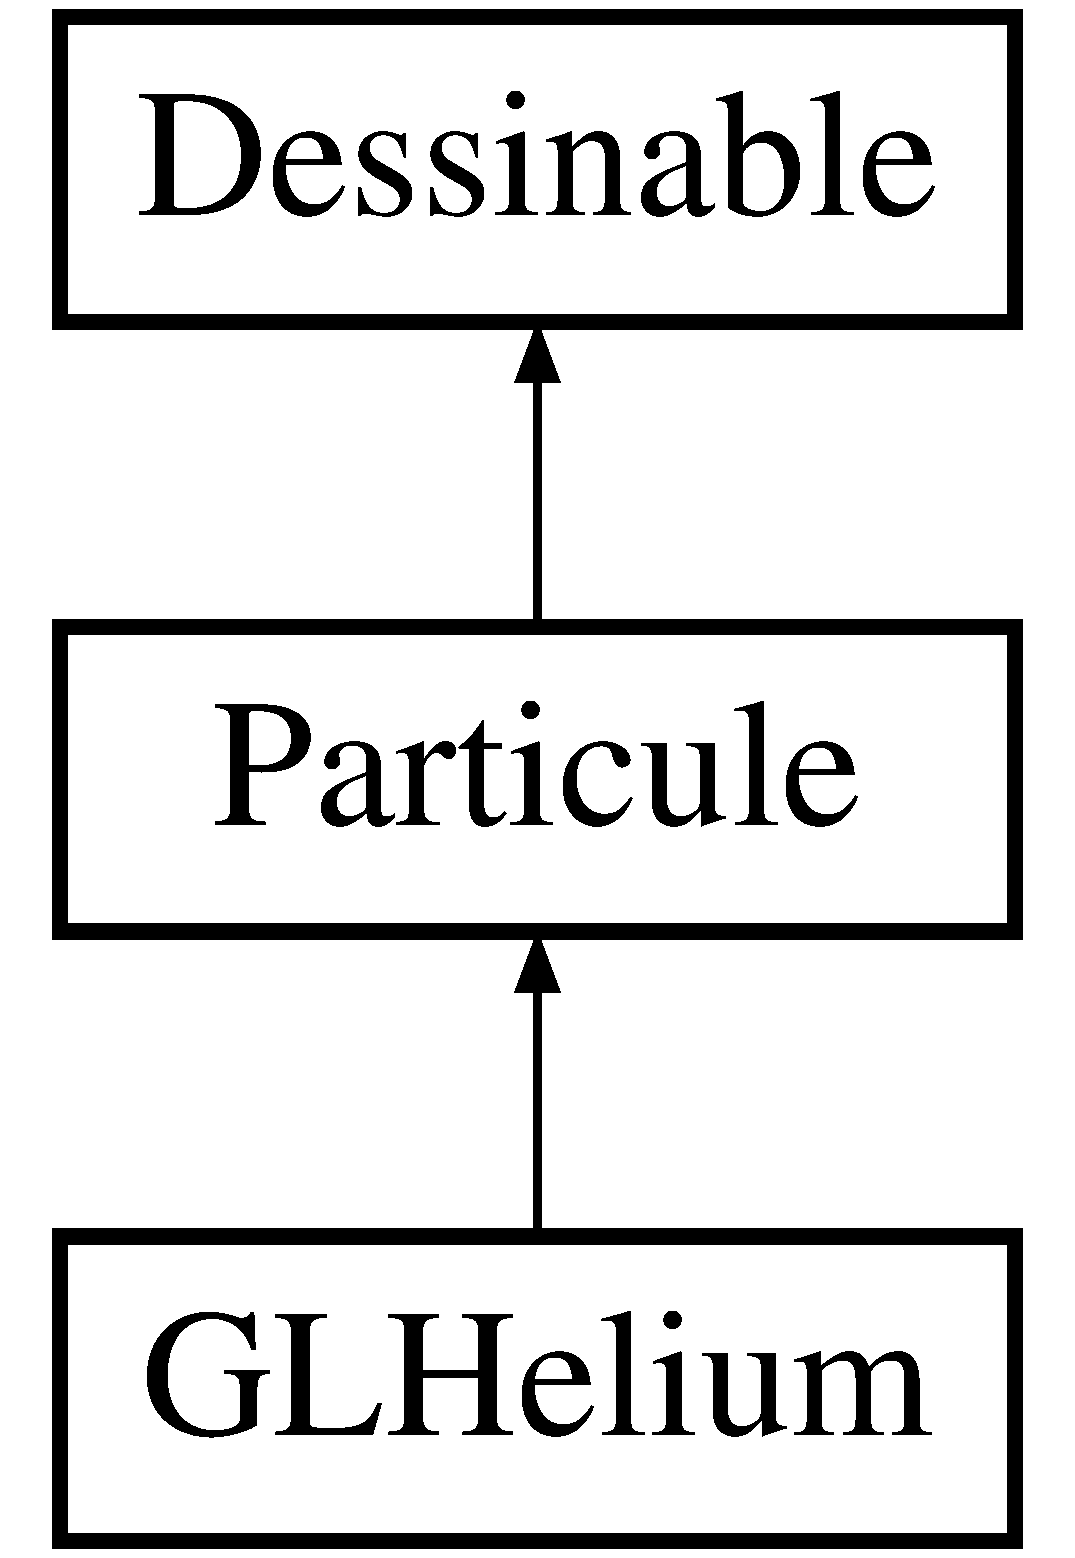
\includegraphics[height=3.000000cm]{class_g_l_helium}
\end{center}
\end{figure}
\subsection*{Fonctions membres publiques}
\begin{DoxyCompactItemize}
\item 
{\bf G\+L\+Helium} ({\bf Vecteur} {\bf position}, {\bf Vecteur} {\bf vitesse})
\begin{DoxyCompactList}\small\item\em Constructeur avec arguments sans la température du système. \end{DoxyCompactList}\item 
{\bf G\+L\+Helium} ({\bf Enceinte} const \&enceinte, {\bf Generateur\+Aleatoire} \&tirage, double temperature)
\begin{DoxyCompactList}\small\item\em Constructeur avec arguments avec la température du système et le tirage aléatoire des vecteurs positions. \end{DoxyCompactList}\item 
virtual {\bf $\sim$\+G\+L\+Helium} ()
\begin{DoxyCompactList}\small\item\em Dstructeurs. \end{DoxyCompactList}\item 
virtual void {\bf evolue} (double dt)
\begin{DoxyCompactList}\small\item\em Prototype de la méthode evolue. \end{DoxyCompactList}\item 
virtual void {\bf dessine} () const 
\begin{DoxyCompactList}\small\item\em Prototype de la méthode evolue. \end{DoxyCompactList}\end{DoxyCompactItemize}
\subsection*{Membres hérités additionnels}


\subsection{Description détaillée}
Prototype de la classe \doxyref{G\+L\+Helium}{p.}{class_g_l_helium}. 

Cette classe est celle qui permet de créer une particule d'helium en Open\+G 

Définition à la ligne {\bf 23} du fichier {\bf G\+L\+Helium.\+h}.



\subsection{Documentation des constructeurs et destructeur}
\index{G\+L\+Helium@{G\+L\+Helium}!G\+L\+Helium@{G\+L\+Helium}}
\index{G\+L\+Helium@{G\+L\+Helium}!G\+L\+Helium@{G\+L\+Helium}}
\subsubsection[{G\+L\+Helium}]{\setlength{\rightskip}{0pt plus 5cm}G\+L\+Helium\+::\+G\+L\+Helium (
\begin{DoxyParamCaption}
\item[{{\bf Vecteur}}]{position, }
\item[{{\bf Vecteur}}]{vitesse}
\end{DoxyParamCaption}
)}\label{class_g_l_helium_ac225aa981f016d8cf08823178e69f1b2}


Constructeur avec arguments sans la température du système. 

sans le paramètre de température, initialise un rayon et une masse à notre particule


\begin{DoxyParams}{Paramètres}
{\em position} & \+: est la position de la particule que l'on souhaite \\
\hline
{\em vitesse} & \+: est la vitesse de la particule que l'on souhaite \\
\hline
\end{DoxyParams}


Définition à la ligne {\bf 20} du fichier {\bf G\+L\+Helium.\+cc}.

\index{G\+L\+Helium@{G\+L\+Helium}!G\+L\+Helium@{G\+L\+Helium}}
\index{G\+L\+Helium@{G\+L\+Helium}!G\+L\+Helium@{G\+L\+Helium}}
\subsubsection[{G\+L\+Helium}]{\setlength{\rightskip}{0pt plus 5cm}G\+L\+Helium\+::\+G\+L\+Helium (
\begin{DoxyParamCaption}
\item[{{\bf Enceinte} const \&}]{enceinte, }
\item[{{\bf Generateur\+Aleatoire} \&}]{tirage, }
\item[{double}]{temperature}
\end{DoxyParamCaption}
)}\label{class_g_l_helium_a259d6f61ae97df566b2e91db34bc97fa}


Constructeur avec arguments avec la température du système et le tirage aléatoire des vecteurs positions. 

sans le paramètre de température, initialise un rayon et une masse à notre particule


\begin{DoxyParams}{Paramètres}
{\em enceinte} & \+: permet de connaitre les dimmensions de l'emceinte pour calculer les positions \\
\hline
{\em tirage} & \+: donne une position aléatoire de la particule dans l'enceinte \\
\hline
{\em gtempérature} & \+: la température que l'on souhaite pour calculer la vitesse \\
\hline
\end{DoxyParams}


Définition à la ligne {\bf 30} du fichier {\bf G\+L\+Helium.\+cc}.

\index{G\+L\+Helium@{G\+L\+Helium}!````~G\+L\+Helium@{$\sim$\+G\+L\+Helium}}
\index{````~G\+L\+Helium@{$\sim$\+G\+L\+Helium}!G\+L\+Helium@{G\+L\+Helium}}
\subsubsection[{$\sim$\+G\+L\+Helium}]{\setlength{\rightskip}{0pt plus 5cm}G\+L\+Helium\+::$\sim$\+G\+L\+Helium (
\begin{DoxyParamCaption}
{}
\end{DoxyParamCaption}
)\hspace{0.3cm}{\ttfamily [virtual]}}\label{class_g_l_helium_a17f9a1bcd3bc8c25b84fe6de8348510c}


Dstructeurs. 



Définition à la ligne {\bf 34} du fichier {\bf G\+L\+Helium.\+cc}.



\subsection{Documentation des fonctions membres}
\index{G\+L\+Helium@{G\+L\+Helium}!dessine@{dessine}}
\index{dessine@{dessine}!G\+L\+Helium@{G\+L\+Helium}}
\subsubsection[{dessine}]{\setlength{\rightskip}{0pt plus 5cm}void G\+L\+Helium\+::dessine (
\begin{DoxyParamCaption}
{}
\end{DoxyParamCaption}
) const\hspace{0.3cm}{\ttfamily [virtual]}}\label{class_g_l_helium_a425b1c773fa42f6e244d4036cbcb6ea3}


Prototype de la méthode evolue. 

dessine la particule de couleur à la position souhaitée par une matrice de translation orange

J'ai remis 10 partout 

Implémente {\bf Dessinable} \doxyref{}{p.}{class_dessinable_aea37dacb2b67d6650a435d72c9a6fe79}.



Définition à la ligne {\bf 55} du fichier {\bf G\+L\+Helium.\+cc}.

\index{G\+L\+Helium@{G\+L\+Helium}!evolue@{evolue}}
\index{evolue@{evolue}!G\+L\+Helium@{G\+L\+Helium}}
\subsubsection[{evolue}]{\setlength{\rightskip}{0pt plus 5cm}void G\+L\+Helium\+::evolue (
\begin{DoxyParamCaption}
\item[{double}]{dt}
\end{DoxyParamCaption}
)\hspace{0.3cm}{\ttfamily [virtual]}}\label{class_g_l_helium_ae26ea4b2eebe39c9d86be7db52e7d507}


Prototype de la méthode evolue. 

appelle la méthode évolue de la classe particule 
\begin{DoxyParams}{Paramètres}
{\em dt} & \+: le pas de temps \\
\hline
\end{DoxyParams}


Réimplémentée à partir de {\bf Particule} \doxyref{}{p.}{class_particule_a7c6a97e2b65d4326d36b6d3b6251b79c}.



Définition à la ligne {\bf 46} du fichier {\bf G\+L\+Helium.\+cc}.



La documentation de cette classe a été générée à partir des fichiers suivants \+:\begin{DoxyCompactItemize}
\item 
/\+Users/burkhard/\+Dropbox/projet d'info/maximilian-\/g065/\+Simulation d'un gaz parfait/{\bf G\+L\+Helium.\+h}\item 
/\+Users/burkhard/\+Dropbox/projet d'info/maximilian-\/g065/\+Simulation d'un gaz parfait/{\bf G\+L\+Helium.\+cc}\end{DoxyCompactItemize}

\section{Référence de la classe G\+L\+Neon}
\label{class_g_l_neon}\index{G\+L\+Neon@{G\+L\+Neon}}


Prototype de la classe \doxyref{G\+L\+Neon}{p.}{class_g_l_neon}.  




{\ttfamily \#include $<$G\+L\+Neon.\+h$>$}

Graphe d'héritage de G\+L\+Neon\+:\begin{figure}[H]
\begin{center}
\leavevmode
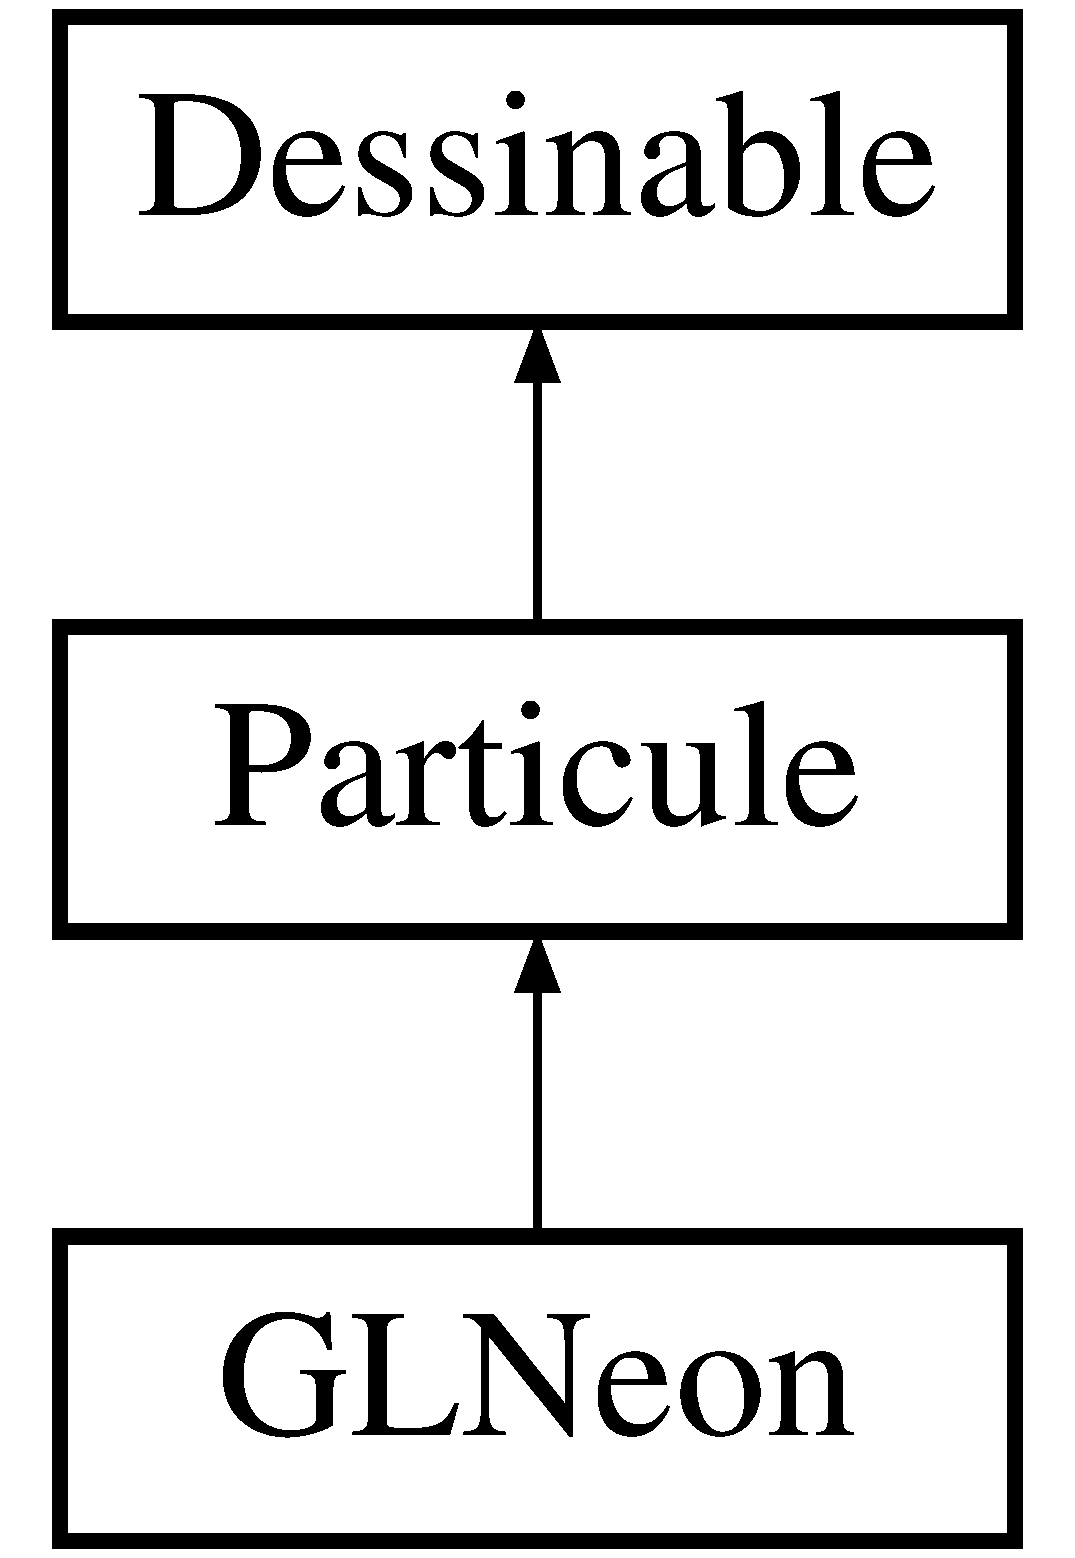
\includegraphics[height=3.000000cm]{class_g_l_neon}
\end{center}
\end{figure}
\subsection*{Fonctions membres publiques}
\begin{DoxyCompactItemize}
\item 
{\bf G\+L\+Neon} ({\bf Vecteur} {\bf position}, {\bf Vecteur} {\bf vitesse})
\begin{DoxyCompactList}\small\item\em Constructeur avec arguments sans la température du système. \end{DoxyCompactList}\item 
{\bf G\+L\+Neon} ({\bf Enceinte} const \&enceinte, {\bf Generateur\+Aleatoire} \&tirage, double temperature)
\begin{DoxyCompactList}\small\item\em Constructeur avec arguments avec la température du système et le tirage aléatoire des vecteurs positions. \end{DoxyCompactList}\item 
virtual {\bf $\sim$\+G\+L\+Neon} ()
\begin{DoxyCompactList}\small\item\em Dstructeurs. \end{DoxyCompactList}\item 
virtual void {\bf evolue} (double dt)
\begin{DoxyCompactList}\small\item\em Prototype de la méthode evolue. \end{DoxyCompactList}\item 
virtual void {\bf dessine} () const 
\begin{DoxyCompactList}\small\item\em Prototype de la méthode evolue. \end{DoxyCompactList}\end{DoxyCompactItemize}
\subsection*{Membres hérités additionnels}


\subsection{Description détaillée}
Prototype de la classe \doxyref{G\+L\+Neon}{p.}{class_g_l_neon}. 

Cette classe est celle qui permet de créer une particule de néon en Open\+G 

Définition à la ligne {\bf 24} du fichier {\bf G\+L\+Neon.\+h}.



\subsection{Documentation des constructeurs et destructeur}
\index{G\+L\+Neon@{G\+L\+Neon}!G\+L\+Neon@{G\+L\+Neon}}
\index{G\+L\+Neon@{G\+L\+Neon}!G\+L\+Neon@{G\+L\+Neon}}
\subsubsection[{G\+L\+Neon}]{\setlength{\rightskip}{0pt plus 5cm}G\+L\+Neon\+::\+G\+L\+Neon (
\begin{DoxyParamCaption}
\item[{{\bf Vecteur}}]{position, }
\item[{{\bf Vecteur}}]{vitesse}
\end{DoxyParamCaption}
)}\label{class_g_l_neon_aab37b6c0656408bbfe9f81e5fcd734ca}


Constructeur avec arguments sans la température du système. 

sans le paramètre de température, initialise un rayon et une masse à notre particule


\begin{DoxyParams}{Paramètres}
{\em position} & \+: est la position de la particule que l'on souhaite \\
\hline
{\em vitesse} & \+: est la vitesse de la particule que l'on souhaite \\
\hline
\end{DoxyParams}


Définition à la ligne {\bf 20} du fichier {\bf G\+L\+Neon.\+cc}.

\index{G\+L\+Neon@{G\+L\+Neon}!G\+L\+Neon@{G\+L\+Neon}}
\index{G\+L\+Neon@{G\+L\+Neon}!G\+L\+Neon@{G\+L\+Neon}}
\subsubsection[{G\+L\+Neon}]{\setlength{\rightskip}{0pt plus 5cm}G\+L\+Neon\+::\+G\+L\+Neon (
\begin{DoxyParamCaption}
\item[{{\bf Enceinte} const \&}]{enceinte, }
\item[{{\bf Generateur\+Aleatoire} \&}]{tirage, }
\item[{double}]{temperature}
\end{DoxyParamCaption}
)}\label{class_g_l_neon_a020084a21670e93d5adae7b1212a1d6c}


Constructeur avec arguments avec la température du système et le tirage aléatoire des vecteurs positions. 

sans le paramètre de température, initialise un rayon et une masse à notre particule


\begin{DoxyParams}{Paramètres}
{\em enceinte} & \+: permet de connaitre les dimmensions de l'emceinte pour calculer les positions \\
\hline
{\em tirage} & \+: donne une position aléatoire de la particule dans l'enceinte \\
\hline
{\em gtempérature} & \+: la température que l'on souhaite pour calculer la vitesse \\
\hline
\end{DoxyParams}


Définition à la ligne {\bf 30} du fichier {\bf G\+L\+Neon.\+cc}.

\index{G\+L\+Neon@{G\+L\+Neon}!````~G\+L\+Neon@{$\sim$\+G\+L\+Neon}}
\index{````~G\+L\+Neon@{$\sim$\+G\+L\+Neon}!G\+L\+Neon@{G\+L\+Neon}}
\subsubsection[{$\sim$\+G\+L\+Neon}]{\setlength{\rightskip}{0pt plus 5cm}G\+L\+Neon\+::$\sim$\+G\+L\+Neon (
\begin{DoxyParamCaption}
{}
\end{DoxyParamCaption}
)\hspace{0.3cm}{\ttfamily [virtual]}}\label{class_g_l_neon_afc70b3a04bdcf3bac3e8c3cf3add399f}


Dstructeurs. 



Définition à la ligne {\bf 34} du fichier {\bf G\+L\+Neon.\+cc}.



\subsection{Documentation des fonctions membres}
\index{G\+L\+Neon@{G\+L\+Neon}!dessine@{dessine}}
\index{dessine@{dessine}!G\+L\+Neon@{G\+L\+Neon}}
\subsubsection[{dessine}]{\setlength{\rightskip}{0pt plus 5cm}void G\+L\+Neon\+::dessine (
\begin{DoxyParamCaption}
{}
\end{DoxyParamCaption}
) const\hspace{0.3cm}{\ttfamily [virtual]}}\label{class_g_l_neon_a9829245529338e0f9f20395bf769f9de}


Prototype de la méthode evolue. 

dessine la particule de couleur à la position souhaitée par une matrice de translation couleur rouge, 100\%

J'ai remis 10 partout 

Implémente {\bf Dessinable} \doxyref{}{p.}{class_dessinable_aea37dacb2b67d6650a435d72c9a6fe79}.



Définition à la ligne {\bf 55} du fichier {\bf G\+L\+Neon.\+cc}.

\index{G\+L\+Neon@{G\+L\+Neon}!evolue@{evolue}}
\index{evolue@{evolue}!G\+L\+Neon@{G\+L\+Neon}}
\subsubsection[{evolue}]{\setlength{\rightskip}{0pt plus 5cm}void G\+L\+Neon\+::evolue (
\begin{DoxyParamCaption}
\item[{double}]{dt}
\end{DoxyParamCaption}
)\hspace{0.3cm}{\ttfamily [virtual]}}\label{class_g_l_neon_a2ecf779982ed593522f8f1defb18d4fb}


Prototype de la méthode evolue. 

appelle la méthode évolue de la classe particule 
\begin{DoxyParams}{Paramètres}
{\em dt} & \+: le pas de temps \\
\hline
\end{DoxyParams}


Réimplémentée à partir de {\bf Particule} \doxyref{}{p.}{class_particule_a7c6a97e2b65d4326d36b6d3b6251b79c}.



Définition à la ligne {\bf 46} du fichier {\bf G\+L\+Neon.\+cc}.



La documentation de cette classe a été générée à partir des fichiers suivants \+:\begin{DoxyCompactItemize}
\item 
/\+Users/burkhard/\+Dropbox/projet d'info/maximilian-\/g065/\+Simulation d'un gaz parfait/{\bf G\+L\+Neon.\+h}\item 
/\+Users/burkhard/\+Dropbox/projet d'info/maximilian-\/g065/\+Simulation d'un gaz parfait/{\bf G\+L\+Neon.\+cc}\end{DoxyCompactItemize}

\section{Référence de la classe G\+U\+I}
\label{class_g_u_i}\index{G\+U\+I@{G\+U\+I}}


Application principale.  




{\ttfamily \#include $<$G\+U\+I.\+h$>$}

Graphe d'héritage de G\+U\+I\+:\begin{figure}[H]
\begin{center}
\leavevmode
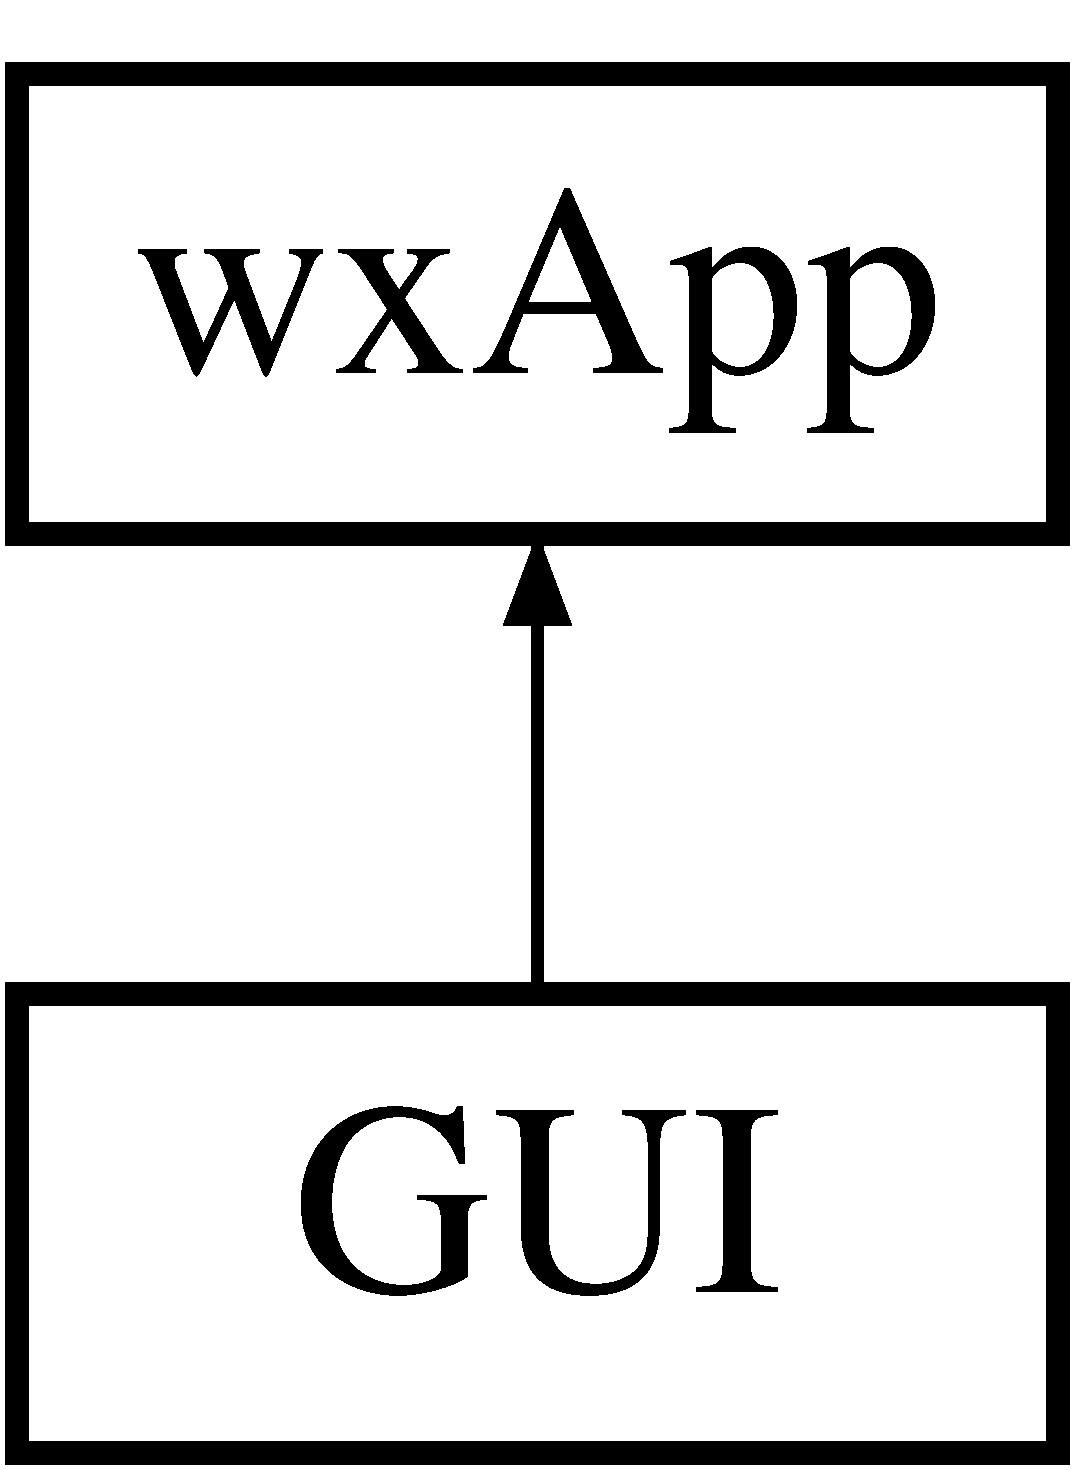
\includegraphics[height=2.000000cm]{class_g_u_i}
\end{center}
\end{figure}
\subsection*{Fonctions membres publiques}
\begin{DoxyCompactItemize}
\item 
bool {\bf On\+Init} ()
\begin{DoxyCompactList}\small\item\em prototype qui lance l'application en appelant les différents constructeurs \end{DoxyCompactList}\end{DoxyCompactItemize}


\subsection{Description détaillée}
Application principale. 

Définition à la ligne {\bf 20} du fichier {\bf G\+U\+I.\+h}.



\subsection{Documentation des fonctions membres}
\index{G\+U\+I@{G\+U\+I}!On\+Init@{On\+Init}}
\index{On\+Init@{On\+Init}!G\+U\+I@{G\+U\+I}}
\subsubsection[{On\+Init}]{\setlength{\rightskip}{0pt plus 5cm}bool G\+U\+I\+::\+On\+Init (
\begin{DoxyParamCaption}
{}
\end{DoxyParamCaption}
)}\label{class_g_u_i_a31f9119b91b3ab5aad63df5d2065a005}


prototype qui lance l'application en appelant les différents constructeurs 

Nous avons décider de faire une interface utilisateur et la première question est où mettre un tel objet ? Ici dans on\+Init. C'est de savoir si on veut créer un système aléatoire ou pas et va le transmettre en arguments pour que la donnée transite jusqu'où elle doit aller \begin{DoxyVerb}\return true si la fenere à pu être créé\end{DoxyVerb}
 variable utile pour enregistrer le choix de l'uitlisateur

permet de poser la question à l'utilisateur pour parameter le systeme ou non si il dit oui, le booléens sera true ! 

Définition à la ligne {\bf 24} du fichier {\bf G\+U\+I.\+cc}.



La documentation de cette classe a été générée à partir des fichiers suivants \+:\begin{DoxyCompactItemize}
\item 
/\+Users/burkhard/\+Dropbox/projet d'info/maximilian-\/g065/\+Simulation d'un gaz parfait/{\bf G\+U\+I.\+h}\item 
/\+Users/burkhard/\+Dropbox/projet d'info/maximilian-\/g065/\+Simulation d'un gaz parfait/{\bf G\+U\+I.\+cc}\end{DoxyCompactItemize}

\section{Référence de la classe T\+X\+T\+Argon\+:\+:h}
\label{class_t_x_t_argon_1_1h}\index{T\+X\+T\+Argon\+::h@{T\+X\+T\+Argon\+::h}}


Représente des atomes d'Argon (version texte)  




{\ttfamily \#include $<$T\+X\+T\+Argon.\+h$>$}



\subsection{Description détaillée}
Représente des atomes d'Argon (version texte) 

\begin{DoxySeeAlso}{Voir également}
Test\+T\+X\+T\+Argon, \doxyref{T\+X\+T\+Helium}{p.}{class_t_x_t_helium}, \doxyref{T\+X\+T\+Neon}{p.}{class_t_x_t_neon} 
\end{DoxySeeAlso}


La documentation de cette classe a été générée à partir du fichier suivant \+:\begin{DoxyCompactItemize}
\item 
/\+Users/burkhard/\+Dropbox/projet d'info/maximilian-\/g065/\+Simulation d'un gaz parfait/{\bf T\+X\+T\+Argon.\+h}\end{DoxyCompactItemize}

\section{Référence de la classe T\+X\+T\+Neon\+:\+:h}
\label{class_t_x_t_neon_1_1h}\index{T\+X\+T\+Neon\+::h@{T\+X\+T\+Neon\+::h}}


Représente des atomes de Neon (version texte)  




{\ttfamily \#include $<$T\+X\+T\+Neon.\+h$>$}



\subsection{Description détaillée}
Représente des atomes de Neon (version texte) 

\begin{DoxySeeAlso}{Voir également}
Test\+T\+X\+T\+Neon, \doxyref{T\+X\+T\+Argon}{p.}{class_t_x_t_argon}, \doxyref{T\+X\+T\+Helium}{p.}{class_t_x_t_helium} 
\end{DoxySeeAlso}


La documentation de cette classe a été générée à partir du fichier suivant \+:\begin{DoxyCompactItemize}
\item 
/\+Users/burkhard/\+Dropbox/projet d'info/maximilian-\/g065/\+Simulation d'un gaz parfait/{\bf T\+X\+T\+Neon.\+h}\end{DoxyCompactItemize}

\section{Référence de la classe T\+X\+T\+Helium\+:\+:h}
\label{class_t_x_t_helium_1_1h}\index{T\+X\+T\+Helium\+::h@{T\+X\+T\+Helium\+::h}}


Représente des atomes d'Helium (version texte)  




{\ttfamily \#include $<$T\+X\+T\+Helium.\+h$>$}



\subsection{Description détaillée}
Représente des atomes d'Helium (version texte) 

\begin{DoxySeeAlso}{Voir également}
Test\+T\+X\+T\+Helium, \doxyref{T\+X\+T\+Argon}{p.}{class_t_x_t_argon}, \doxyref{T\+X\+T\+Neon}{p.}{class_t_x_t_neon} 
\end{DoxySeeAlso}


La documentation de cette classe a été générée à partir du fichier suivant \+:\begin{DoxyCompactItemize}
\item 
/\+Users/burkhard/\+Dropbox/projet d'info/maximilian-\/g065/\+Simulation d'un gaz parfait/{\bf T\+X\+T\+Helium.\+h}\end{DoxyCompactItemize}

\section{Référence de la classe Particule}
\label{class_particule}\index{Particule@{Particule}}


Classe mère dont hérite toutes les classes de type \+: T\+X\+T\+Nom et G\+L\+Nom Représentation d'une particule (ici version graphique)  




{\ttfamily \#include $<$Particule.\+h$>$}

Graphe d'héritage de Particule\+:\begin{figure}[H]
\begin{center}
\leavevmode
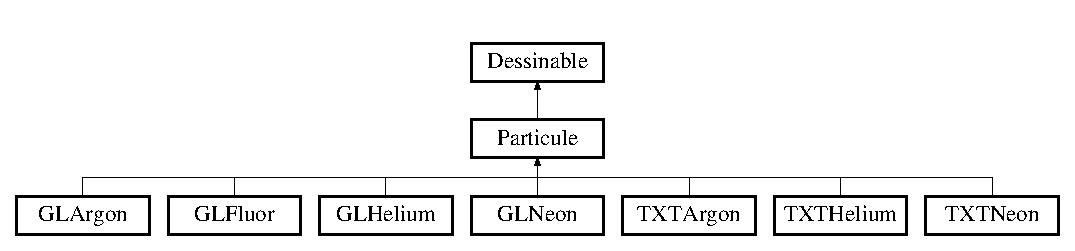
\includegraphics[height=2.926829cm]{class_particule}
\end{center}
\end{figure}
\subsection*{Fonctions membres publiques}
\begin{DoxyCompactItemize}
\item 
{\bf Particule} ()
\begin{DoxyCompactList}\small\item\em Constructeur par défaut. \end{DoxyCompactList}\item 
{\bf Particule} ({\bf Vecteur} {\bf position}, {\bf Vecteur} {\bf vitesse}, double {\bf masse}, double {\bf rayon})
\begin{DoxyCompactList}\small\item\em Constructeur. \end{DoxyCompactList}\item 
{\bf Particule} ({\bf Enceinte} const \&enceinte, {\bf Generateur\+Aleatoire} \&tirage, double temperature, double {\bf masse}, double {\bf rayon})
\begin{DoxyCompactList}\small\item\em Constructeur. \end{DoxyCompactList}\item 
{\bf Vecteur} {\bf get\+Position} () const 
\begin{DoxyCompactList}\small\item\em Getter de position de la particule. \end{DoxyCompactList}\item 
std\+::ostream \& {\bf afficher} (std\+::ostream \&sortie) const 
\begin{DoxyCompactList}\small\item\em Permet d'afficher les différents attributs de la particule. \end{DoxyCompactList}\item 
virtual void {\bf evolue} (double dt)
\begin{DoxyCompactList}\small\item\em S'occupe de faire évoluer la particule d'un temps dt. \end{DoxyCompactList}\item 
void {\bf gere\+\_\+sorties} ({\bf Enceinte} const \&enceinte)
\begin{DoxyCompactList}\small\item\em Gére les sorties de l'enceinte. \end{DoxyCompactList}\item 
{\bf Vecteur} {\bf pavage\+Cubique} (double espsilon) const 
\begin{DoxyCompactList}\small\item\em Calcul le pavage cubique autour d'une particule. \end{DoxyCompactList}\item 
void {\bf collision} ({\bf Particule} \&p, {\bf Generateur\+Aleatoire} \&tirage)
\begin{DoxyCompactList}\small\item\em Effectue la collision de deux particules. \end{DoxyCompactList}\item 
double {\bf get\+\_\+rayon} ()
\begin{DoxyCompactList}\small\item\em Getter. \end{DoxyCompactList}\end{DoxyCompactItemize}
\subsection*{Attributs protégés}
\begin{DoxyCompactItemize}
\item 
{\bf Vecteur} {\bf position}
\item 
{\bf Vecteur} {\bf vitesse}
\item 
double const {\bf masse}
\item 
double const {\bf rayon}
\end{DoxyCompactItemize}


\subsection{Description détaillée}
Classe mère dont hérite toutes les classes de type \+: T\+X\+T\+Nom et G\+L\+Nom Représentation d'une particule (ici version graphique) 

C'est une classe virtuelle pure, on ne peut donc pas créer d'instances de cette classe car il n'est pas logique de créer l'objet générale mais plutôt des classes spécialisées. Elle permet d'avoir une structure générale et des méthodes que chacunes des particules devra redéfinir. 

Définition à la ligne {\bf 27} du fichier {\bf Particule.\+h}.



\subsection{Documentation des constructeurs et destructeur}
\index{Particule@{Particule}!Particule@{Particule}}
\index{Particule@{Particule}!Particule@{Particule}}
\subsubsection[{Particule}]{\setlength{\rightskip}{0pt plus 5cm}Particule\+::\+Particule (
\begin{DoxyParamCaption}
{}
\end{DoxyParamCaption}
)}\label{class_particule_ac19d3be1dc7c116c39afedfbe34f99a7}


Constructeur par défaut. 

Initialise tous les paramètres de type vecteur comme des vecteurs nuls et ceux de type double à 0 

Définition à la ligne {\bf 18} du fichier {\bf Particule.\+cc}.

\index{Particule@{Particule}!Particule@{Particule}}
\index{Particule@{Particule}!Particule@{Particule}}
\subsubsection[{Particule}]{\setlength{\rightskip}{0pt plus 5cm}Particule\+::\+Particule (
\begin{DoxyParamCaption}
\item[{{\bf Vecteur}}]{position, }
\item[{{\bf Vecteur}}]{vitesse, }
\item[{double}]{masse, }
\item[{double}]{rayon}
\end{DoxyParamCaption}
)}\label{class_particule_ae77bbc2fbc9a212d4eb03d075873b687}


Constructeur. 

Permet d'initialiser une particule en fournissant une position, une vitesse, une masse et un rayon 
\begin{DoxyParams}{Paramètres}
{\em position} & \doxyref{Vecteur}{p.}{class_vecteur} indiquant la position de la particule \\
\hline
{\em vitesse} & \doxyref{Vecteur}{p.}{class_vecteur} indiquant la vitesse de la particule \\
\hline
{\em masse} & Nombre réel indiquant la masse de la particule \\
\hline
{\em rayon} & Nombre réel indiquant le rayon de la particule \\
\hline
\end{DoxyParams}


Définition à la ligne {\bf 27} du fichier {\bf Particule.\+cc}.

\index{Particule@{Particule}!Particule@{Particule}}
\index{Particule@{Particule}!Particule@{Particule}}
\subsubsection[{Particule}]{\setlength{\rightskip}{0pt plus 5cm}Particule\+::\+Particule (
\begin{DoxyParamCaption}
\item[{{\bf Enceinte} const \&}]{enceinte, }
\item[{{\bf Generateur\+Aleatoire} \&}]{tirage, }
\item[{double}]{temperature, }
\item[{double}]{masse, }
\item[{double}]{rayon}
\end{DoxyParamCaption}
)}\label{class_particule_aeb9d4042dfb2df93f28066f8556ccafc}


Constructeur. 

Permet d'initialiser aléatoirement la position et la vitesse de la particule sur une enceinte 
\begin{DoxyParams}{Paramètres}
{\em enceinte} & \doxyref{Enceinte}{p.}{class_enceinte} dans laquelle doit se trouver la particule \\
\hline
\end{DoxyParams}


Définition à la ligne {\bf 33} du fichier {\bf Particule.\+cc}.



\subsection{Documentation des fonctions membres}
\index{Particule@{Particule}!afficher@{afficher}}
\index{afficher@{afficher}!Particule@{Particule}}
\subsubsection[{afficher}]{\setlength{\rightskip}{0pt plus 5cm}ostream \& Particule\+::afficher (
\begin{DoxyParamCaption}
\item[{std\+::ostream \&}]{sortie}
\end{DoxyParamCaption}
) const}\label{class_particule_a95c61ca247604a3107cbad1b22a6f9a6}


Permet d'afficher les différents attributs de la particule. 


\begin{DoxyParams}{Paramètres}
{\em sortie} & ostream sur lequel l'affichage s'effectue \\
\hline
\end{DoxyParams}
\begin{DoxyReturn}{Renvoie}
ostream sur lequel l'affichage a été fait 
\end{DoxyReturn}


Définition à la ligne {\bf 57} du fichier {\bf Particule.\+cc}.

\index{Particule@{Particule}!collision@{collision}}
\index{collision@{collision}!Particule@{Particule}}
\subsubsection[{collision}]{\setlength{\rightskip}{0pt plus 5cm}void Particule\+::collision (
\begin{DoxyParamCaption}
\item[{{\bf Particule} \&}]{p, }
\item[{{\bf Generateur\+Aleatoire} \&}]{tirage}
\end{DoxyParamCaption}
)}\label{class_particule_a91283a1702ac9f40728e58613ad97ac9}


Effectue la collision de deux particules. 


\begin{DoxyParams}{Paramètres}
{\em p} & \doxyref{Particule}{p.}{class_particule} avec laquelle $\ast$this entre en collision \\
\hline
{\em tirage} & \doxyref{Generateur\+Aleatoire}{p.}{class_generateur_aleatoire} permettant d'effectuer différents tirages de nombres dans la méthode \\
\hline
\end{DoxyParams}


Définition à la ligne {\bf 132} du fichier {\bf Particule.\+cc}.

\index{Particule@{Particule}!evolue@{evolue}}
\index{evolue@{evolue}!Particule@{Particule}}
\subsubsection[{evolue}]{\setlength{\rightskip}{0pt plus 5cm}void Particule\+::evolue (
\begin{DoxyParamCaption}
\item[{double}]{dt}
\end{DoxyParamCaption}
)\hspace{0.3cm}{\ttfamily [virtual]}}\label{class_particule_a7c6a97e2b65d4326d36b6d3b6251b79c}


S'occupe de faire évoluer la particule d'un temps dt. 


\begin{DoxyParams}{Paramètres}
{\em dt} & Pas de temps \\
\hline
\end{DoxyParams}


Réimplémentée dans {\bf G\+L\+Fluor} \doxyref{}{p.}{class_g_l_fluor_a9fbbc20c3f158575d39fce6c9ca85931}, {\bf G\+L\+Argon} \doxyref{}{p.}{class_g_l_argon_a18a22f3feb53956d69c52031d4f86b96}, {\bf G\+L\+Neon} \doxyref{}{p.}{class_g_l_neon_a2ecf779982ed593522f8f1defb18d4fb}, et {\bf G\+L\+Helium} \doxyref{}{p.}{class_g_l_helium_ae26ea4b2eebe39c9d86be7db52e7d507}.



Définition à la ligne {\bf 64} du fichier {\bf Particule.\+cc}.

\index{Particule@{Particule}!gere\+\_\+sorties@{gere\+\_\+sorties}}
\index{gere\+\_\+sorties@{gere\+\_\+sorties}!Particule@{Particule}}
\subsubsection[{gere\+\_\+sorties}]{\setlength{\rightskip}{0pt plus 5cm}void Particule\+::gere\+\_\+sorties (
\begin{DoxyParamCaption}
\item[{{\bf Enceinte} const \&}]{enceinte}
\end{DoxyParamCaption}
)}\label{class_particule_abdd1239a60f7099dcecd8a8269ce1b4d}


Gére les sorties de l'enceinte. 

Détermine si la particule sort ou non de l'enceinte. Si elle sort effectivement (c'est à dire le B\+O\+R\+D de la particule est sorti de l'enceinte), on change les Vecteurs position et vitesse en conséquence 
\begin{DoxyParams}{Paramètres}
{\em enceinte} & \doxyref{Enceinte}{p.}{class_enceinte} dans laquelle la particule se trouve et doit rester \\
\hline
\end{DoxyParams}


Définition à la ligne {\bf 73} du fichier {\bf Particule.\+cc}.

\index{Particule@{Particule}!get\+\_\+rayon@{get\+\_\+rayon}}
\index{get\+\_\+rayon@{get\+\_\+rayon}!Particule@{Particule}}
\subsubsection[{get\+\_\+rayon}]{\setlength{\rightskip}{0pt plus 5cm}double Particule\+::get\+\_\+rayon (
\begin{DoxyParamCaption}
{}
\end{DoxyParamCaption}
)}\label{class_particule_a50d7ab965780895a97d00a13cbb2dfde}


Getter. 

Utile pour déterminer le pas d'espace epsilon du systeme \begin{DoxyReturn}{Renvoie}
Retourne le rayon de la particule 
\end{DoxyReturn}


Définition à la ligne {\bf 150} du fichier {\bf Particule.\+cc}.

\index{Particule@{Particule}!get\+Position@{get\+Position}}
\index{get\+Position@{get\+Position}!Particule@{Particule}}
\subsubsection[{get\+Position}]{\setlength{\rightskip}{0pt plus 5cm}{\bf Vecteur} Particule\+::get\+Position (
\begin{DoxyParamCaption}
{}
\end{DoxyParamCaption}
) const}\label{class_particule_a1c4d2cb7bc6a5357d459ac941d1fd8e1}


Getter de position de la particule. 

Utile pour donner la postion aux méthodes de translation dans dessine de chaque particule \begin{DoxyReturn}{Renvoie}
Retourne le vecteur position de la particule 
\end{DoxyReturn}


Définition à la ligne {\bf 51} du fichier {\bf Particule.\+cc}.

\index{Particule@{Particule}!pavage\+Cubique@{pavage\+Cubique}}
\index{pavage\+Cubique@{pavage\+Cubique}!Particule@{Particule}}
\subsubsection[{pavage\+Cubique}]{\setlength{\rightskip}{0pt plus 5cm}{\bf Vecteur} Particule\+::pavage\+Cubique (
\begin{DoxyParamCaption}
\item[{double}]{epsilon}
\end{DoxyParamCaption}
) const}\label{class_particule_a8e04aa83dad72fac99f3401523995c95}


Calcul le pavage cubique autour d'une particule. 


\begin{DoxyParams}{Paramètres}
{\em epsilon} & Pas d'espace \\
\hline
\end{DoxyParams}
\begin{DoxyReturn}{Renvoie}
Retourne un vecteur qui représente le pavage cubique autour de la particule (et peut-\/être comparé avec le vecteur de pavage d'une autre particule) 
\end{DoxyReturn}


Définition à la ligne {\bf 124} du fichier {\bf Particule.\+cc}.



\subsection{Documentation des données membres}
\index{Particule@{Particule}!masse@{masse}}
\index{masse@{masse}!Particule@{Particule}}
\subsubsection[{masse}]{\setlength{\rightskip}{0pt plus 5cm}double const Particule\+::masse\hspace{0.3cm}{\ttfamily [protected]}}\label{class_particule_a0ee84f95c71e804553be406f4fa098ed}
Nombre réel représentant la masse de la particule (nécessaire pour le calcul des nouvelles vitesses lors d'une collision) 

Définition à la ligne {\bf 38} du fichier {\bf Particule.\+h}.

\index{Particule@{Particule}!position@{position}}
\index{position@{position}!Particule@{Particule}}
\subsubsection[{position}]{\setlength{\rightskip}{0pt plus 5cm}{\bf Vecteur} Particule\+::position\hspace{0.3cm}{\ttfamily [protected]}}\label{class_particule_ac4ebb70316848d69fb600ee2d64e12bf}
\doxyref{Vecteur}{p.}{class_vecteur} représentant la position de la particule dans l'enceinte 

Définition à la ligne {\bf 34} du fichier {\bf Particule.\+h}.

\index{Particule@{Particule}!rayon@{rayon}}
\index{rayon@{rayon}!Particule@{Particule}}
\subsubsection[{rayon}]{\setlength{\rightskip}{0pt plus 5cm}double const Particule\+::rayon\hspace{0.3cm}{\ttfamily [protected]}}\label{class_particule_a77a5348e4ed4309e9c4bf2624afa5804}
Nombre réel représentant le rayon de la particule (nécessaire pour déterminer si des particules entrent en collision) 

Définition à la ligne {\bf 40} du fichier {\bf Particule.\+h}.

\index{Particule@{Particule}!vitesse@{vitesse}}
\index{vitesse@{vitesse}!Particule@{Particule}}
\subsubsection[{vitesse}]{\setlength{\rightskip}{0pt plus 5cm}{\bf Vecteur} Particule\+::vitesse\hspace{0.3cm}{\ttfamily [protected]}}\label{class_particule_af9eef46b603338ea88b238a777041204}
\doxyref{Vecteur}{p.}{class_vecteur} représentant la vitesse de la particule 

Définition à la ligne {\bf 36} du fichier {\bf Particule.\+h}.



La documentation de cette classe a été générée à partir des fichiers suivants \+:\begin{DoxyCompactItemize}
\item 
/\+Users/burkhard/\+Dropbox/projet d'info/maximilian-\/g065/\+Simulation d'un gaz parfait/{\bf Particule.\+h}\item 
/\+Users/burkhard/\+Dropbox/projet d'info/maximilian-\/g065/\+Simulation d'un gaz parfait/{\bf Particule.\+cc}\end{DoxyCompactItemize}

\section{Référence de la classe Systeme}
\label{class_systeme}\index{Systeme@{Systeme}}


Permet de créer, de dessiner et de faire évoluer des objets de type \doxyref{Systeme}{p.}{class_systeme} formés d'une enceinte et de particules.  




{\ttfamily \#include $<$Systeme.\+h$>$}

Graphe d'héritage de Systeme\+:\begin{figure}[H]
\begin{center}
\leavevmode
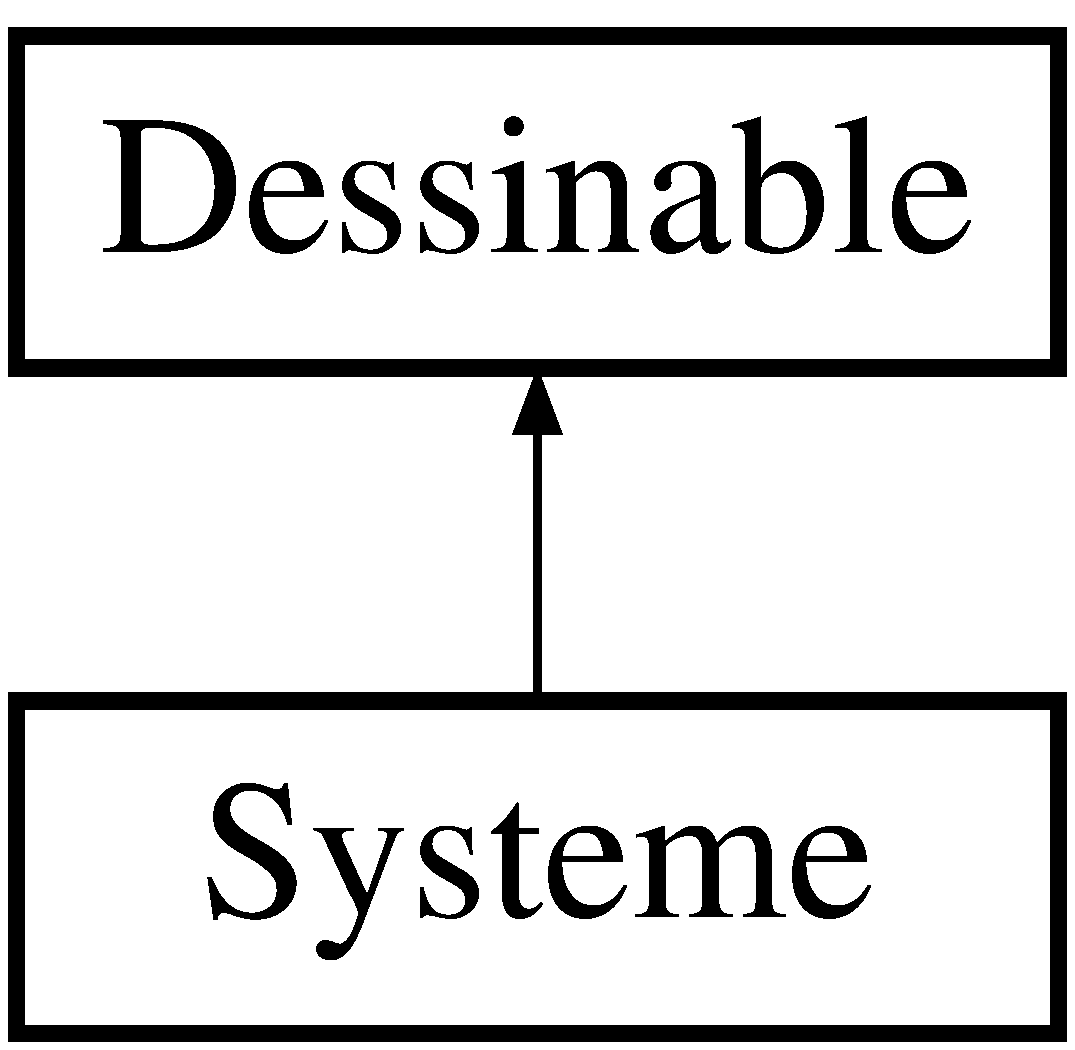
\includegraphics[height=2.000000cm]{class_systeme}
\end{center}
\end{figure}
\subsection*{Fonctions membres publiques}
\begin{DoxyCompactItemize}
\item 
{\bf Systeme} ()
\begin{DoxyCompactList}\small\item\em Constructeur par défaut. \end{DoxyCompactList}\item 
{\bf Systeme} (bool reglage)
\begin{DoxyCompactList}\small\item\em Constructeur. \end{DoxyCompactList}\item 
{\bf Systeme} (double largeur, double longueur, double hauteur, double temperature)
\begin{DoxyCompactList}\small\item\em Constructeur. \end{DoxyCompactList}\item 
{\bf $\sim$\+Systeme} ()
\begin{DoxyCompactList}\small\item\em Destructeur. \end{DoxyCompactList}\item 
void {\bf ajouter\+Argon} (unsigned int nbr\+\_\+argon, bool canon=false)
\begin{DoxyCompactList}\small\item\em Permet l'ajout de nbr\+\_\+argon particules d'Argon. \end{DoxyCompactList}\item 
void {\bf ajouter\+Fluor} (unsigned int nbr\+\_\+fluor, bool canon=false)
\begin{DoxyCompactList}\small\item\em Permet l'ajout de nbr\+\_\+fluor particules de Fluor. \end{DoxyCompactList}\item 
void {\bf ajouter\+Helium} (unsigned int nbr\+\_\+helium, bool canon=false)
\begin{DoxyCompactList}\small\item\em Permet l'ajout de nbr\+\_\+helium particules d'Helium. \end{DoxyCompactList}\item 
void {\bf ajouter\+Neon} (unsigned int nbr\+\_\+neon, bool canon=false)
\begin{DoxyCompactList}\small\item\em Permet l'ajout de nbr\+\_\+neon particules de Neon. \end{DoxyCompactList}\item 
void {\bf dessine} () const override
\begin{DoxyCompactList}\small\item\em Dessine le systeme (version graphique) \end{DoxyCompactList}\item 
void {\bf evolue} (double dt)
\begin{DoxyCompactList}\small\item\em Evolue le systeme d'un temps dt. \end{DoxyCompactList}\end{DoxyCompactItemize}


\subsection{Description détaillée}
Permet de créer, de dessiner et de faire évoluer des objets de type \doxyref{Systeme}{p.}{class_systeme} formés d'une enceinte et de particules. 

Définition à la ligne {\bf 23} du fichier {\bf Systeme.\+h}.



\subsection{Documentation des constructeurs et destructeur}
\index{Systeme@{Systeme}!Systeme@{Systeme}}
\index{Systeme@{Systeme}!Systeme@{Systeme}}
\subsubsection[{Systeme}]{\setlength{\rightskip}{0pt plus 5cm}Systeme\+::\+Systeme (
\begin{DoxyParamCaption}
{}
\end{DoxyParamCaption}
)}\label{class_systeme_a2599ade4fd47e65b7192d227f60a5482}


Constructeur par défaut. 

Initialise un nombre aléatoire de particules et dans une enceinte par défaut à la température normale 

Définition à la ligne {\bf 27} du fichier {\bf Systeme.\+cc}.

\index{Systeme@{Systeme}!Systeme@{Systeme}}
\index{Systeme@{Systeme}!Systeme@{Systeme}}
\subsubsection[{Systeme}]{\setlength{\rightskip}{0pt plus 5cm}Systeme\+::\+Systeme (
\begin{DoxyParamCaption}
\item[{bool}]{reglage}
\end{DoxyParamCaption}
)}\label{class_systeme_a12e7a9debbec8334b00173e8c93f9f92}


Constructeur. 

Ce constructeur permet à l'utilisateur de paramétrer lui même le systeme au lancement du programme grâce à une interface graphique.


\begin{DoxyParams}{Paramètres}
{\em reglage} & booléen permettant de différencier l'initialisation par défaut et l'initialisation paramétrée \\
\hline
\end{DoxyParams}


Définition à la ligne {\bf 37} du fichier {\bf Systeme.\+cc}.

\index{Systeme@{Systeme}!Systeme@{Systeme}}
\index{Systeme@{Systeme}!Systeme@{Systeme}}
\subsubsection[{Systeme}]{\setlength{\rightskip}{0pt plus 5cm}Systeme\+::\+Systeme (
\begin{DoxyParamCaption}
\item[{double}]{largeur, }
\item[{double}]{longueur, }
\item[{double}]{hauteur, }
\item[{double}]{temperature}
\end{DoxyParamCaption}
)}\label{class_systeme_af1350122550243c381d6ff5d2b4ef38c}


Constructeur. 

Permet d'initialiser le systeme en fournissant tous les paramètres avant le lancement du programme. Les particules elles sont initialisées complètement au hasard. 
\begin{DoxyParams}{Paramètres}
{\em largeur} & Largeur de l'enceinte \\
\hline
{\em longueur} & Longueur de l'enceinte \\
\hline
{\em hauteur} & Hauteur de l'enceinte \\
\hline
{\em temperature} & Température du système \\
\hline
\end{DoxyParams}


Définition à la ligne {\bf 79} du fichier {\bf Systeme.\+cc}.

\index{Systeme@{Systeme}!````~Systeme@{$\sim$\+Systeme}}
\index{````~Systeme@{$\sim$\+Systeme}!Systeme@{Systeme}}
\subsubsection[{$\sim$\+Systeme}]{\setlength{\rightskip}{0pt plus 5cm}Systeme\+::$\sim$\+Systeme (
\begin{DoxyParamCaption}
{}
\end{DoxyParamCaption}
)}\label{class_systeme_ae5b0d713664daee67f170ddc0bdf5c4f}


Destructeur. 

j'ai enlevé la valeur par défaut parce que conceptuellement c'est mieux, on initialise rien (hasard total) ou tout (determination totale)

Permet de libérer la mémoire allouée au moment de la création des unique\+\_\+ptr$<$\+Particule$>$ 

Définition à la ligne {\bf 84} du fichier {\bf Systeme.\+cc}.



\subsection{Documentation des fonctions membres}
\index{Systeme@{Systeme}!ajouter\+Argon@{ajouter\+Argon}}
\index{ajouter\+Argon@{ajouter\+Argon}!Systeme@{Systeme}}
\subsubsection[{ajouter\+Argon}]{\setlength{\rightskip}{0pt plus 5cm}void Systeme\+::ajouter\+Argon (
\begin{DoxyParamCaption}
\item[{unsigned int}]{nbr\+\_\+argon, }
\item[{bool}]{canon = {\ttfamily false}}
\end{DoxyParamCaption}
)}\label{class_systeme_a8a1047862e11ebfe4b267dbc5ab67a17}


Permet l'ajout de nbr\+\_\+argon particules d'Argon. 


\begin{DoxyParams}{Paramètres}
{\em nbr\+\_\+argon} & Nombre de particules d'Argon à ajouter au système \\
\hline
{\em canon} & booléen permettant de déterminer la manière dont l'ajout doit se faire \+: true -\/$>$ tire de canon = ajout d'une file de particule allant toutes dans la même direction false -\/$>$ initialisation aléatoire de la position et de la vitesse de chaque particule \\
\hline
\end{DoxyParams}


Définition à la ligne {\bf 164} du fichier {\bf Systeme.\+cc}.

\index{Systeme@{Systeme}!ajouter\+Fluor@{ajouter\+Fluor}}
\index{ajouter\+Fluor@{ajouter\+Fluor}!Systeme@{Systeme}}
\subsubsection[{ajouter\+Fluor}]{\setlength{\rightskip}{0pt plus 5cm}void Systeme\+::ajouter\+Fluor (
\begin{DoxyParamCaption}
\item[{unsigned int}]{nbr\+\_\+fluor, }
\item[{bool}]{canon = {\ttfamily false}}
\end{DoxyParamCaption}
)}\label{class_systeme_a57d47c92404c5ebb87724545a750b445}


Permet l'ajout de nbr\+\_\+fluor particules de Fluor. 


\begin{DoxyParams}{Paramètres}
{\em nbr\+\_\+fluor} & Nombre de particules de Fluor à ajouter au système \\
\hline
{\em canon} & booléen permettant de déterminer la manière dont l'ajout doit se faire \+: true -\/$>$ tire de canon = ajout d'une file de particule allant toutes dans la même direction false -\/$>$ initialisation aléatoire de la position et de la vitesse de chaque particule \\
\hline
\end{DoxyParams}


Définition à la ligne {\bf 185} du fichier {\bf Systeme.\+cc}.

\index{Systeme@{Systeme}!ajouter\+Helium@{ajouter\+Helium}}
\index{ajouter\+Helium@{ajouter\+Helium}!Systeme@{Systeme}}
\subsubsection[{ajouter\+Helium}]{\setlength{\rightskip}{0pt plus 5cm}void Systeme\+::ajouter\+Helium (
\begin{DoxyParamCaption}
\item[{unsigned int}]{nbr\+\_\+helium, }
\item[{bool}]{canon = {\ttfamily false}}
\end{DoxyParamCaption}
)}\label{class_systeme_ad99fa9b3d52815b1c24c2e886291fa45}


Permet l'ajout de nbr\+\_\+helium particules d'Helium. 


\begin{DoxyParams}{Paramètres}
{\em nbr\+\_\+helium} & Nombre de particules d'Helium à ajouter au système \\
\hline
{\em canon} & booléen permettant de déterminer la manière dont l'ajout doit se faire \+: true -\/$>$ tire de canon = ajout d'une file de particule allant toutes dans la même direction false -\/$>$ initialisation aléatoire de la position et de la vitesse de chaque particule \\
\hline
\end{DoxyParams}


Définition à la ligne {\bf 206} du fichier {\bf Systeme.\+cc}.

\index{Systeme@{Systeme}!ajouter\+Neon@{ajouter\+Neon}}
\index{ajouter\+Neon@{ajouter\+Neon}!Systeme@{Systeme}}
\subsubsection[{ajouter\+Neon}]{\setlength{\rightskip}{0pt plus 5cm}void Systeme\+::ajouter\+Neon (
\begin{DoxyParamCaption}
\item[{unsigned int}]{nbr\+\_\+neon, }
\item[{bool}]{canon = {\ttfamily false}}
\end{DoxyParamCaption}
)}\label{class_systeme_ae08dde7f90dfa367d96be1351f7c8c14}


Permet l'ajout de nbr\+\_\+neon particules de Neon. 


\begin{DoxyParams}{Paramètres}
{\em nbr\+\_\+neon} & Nombre de particules de Neon à ajouter au système \\
\hline
{\em canon} & booléen permettant de déterminer la manière dont l'ajout doit se faire \+: true -\/$>$ tire de canon = ajout d'une file de particule allant toutes dans la même direction false -\/$>$ initialisation aléatoire de la position et de la vitesse de chaque particule \\
\hline
\end{DoxyParams}


Définition à la ligne {\bf 227} du fichier {\bf Systeme.\+cc}.

\index{Systeme@{Systeme}!dessine@{dessine}}
\index{dessine@{dessine}!Systeme@{Systeme}}
\subsubsection[{dessine}]{\setlength{\rightskip}{0pt plus 5cm}void Systeme\+::dessine (
\begin{DoxyParamCaption}
{}
\end{DoxyParamCaption}
) const\hspace{0.3cm}{\ttfamily [override]}, {\ttfamily [virtual]}}\label{class_systeme_abc34a6c64e42d303be77d5df97ff377f}


Dessine le systeme (version graphique) 

Dessine l'enceinte, le canon et l'ensemble des particules du systeme 

Implémente {\bf Dessinable} \doxyref{}{p.}{class_dessinable_aea37dacb2b67d6650a435d72c9a6fe79}.



Définition à la ligne {\bf 99} du fichier {\bf Systeme.\+cc}.

\index{Systeme@{Systeme}!evolue@{evolue}}
\index{evolue@{evolue}!Systeme@{Systeme}}
\subsubsection[{evolue}]{\setlength{\rightskip}{0pt plus 5cm}void Systeme\+::evolue (
\begin{DoxyParamCaption}
\item[{double}]{dt}
\end{DoxyParamCaption}
)}\label{class_systeme_a3308846e3013176c71954ba5e3ae23d1}


Evolue le systeme d'un temps dt. 

Evolution déterministe sans sauvegarde. Pour chaque particule \+: on l'évolue, puis on regarde si elle sort de l'enceinte et enfin on regarde si elle entre en collision avec une autre particule


\begin{DoxyParams}{Paramètres}
{\em dt} & Pas de temps \\
\hline
\end{DoxyParams}


Définition à la ligne {\bf 126} du fichier {\bf Systeme.\+cc}.



La documentation de cette classe a été générée à partir des fichiers suivants \+:\begin{DoxyCompactItemize}
\item 
/\+Users/burkhard/\+Dropbox/projet d'info/maximilian-\/g065/\+Simulation d'un gaz parfait/{\bf Systeme.\+h}\item 
/\+Users/burkhard/\+Dropbox/projet d'info/maximilian-\/g065/\+Simulation d'un gaz parfait/{\bf Systeme.\+cc}\end{DoxyCompactItemize}

\section{Référence de la classe T\+X\+T\+Argon}
\label{class_t_x_t_argon}\index{T\+X\+T\+Argon@{T\+X\+T\+Argon}}


{\ttfamily \#include $<$T\+X\+T\+Argon.\+h$>$}

Graphe d'héritage de T\+X\+T\+Argon\+:\begin{figure}[H]
\begin{center}
\leavevmode
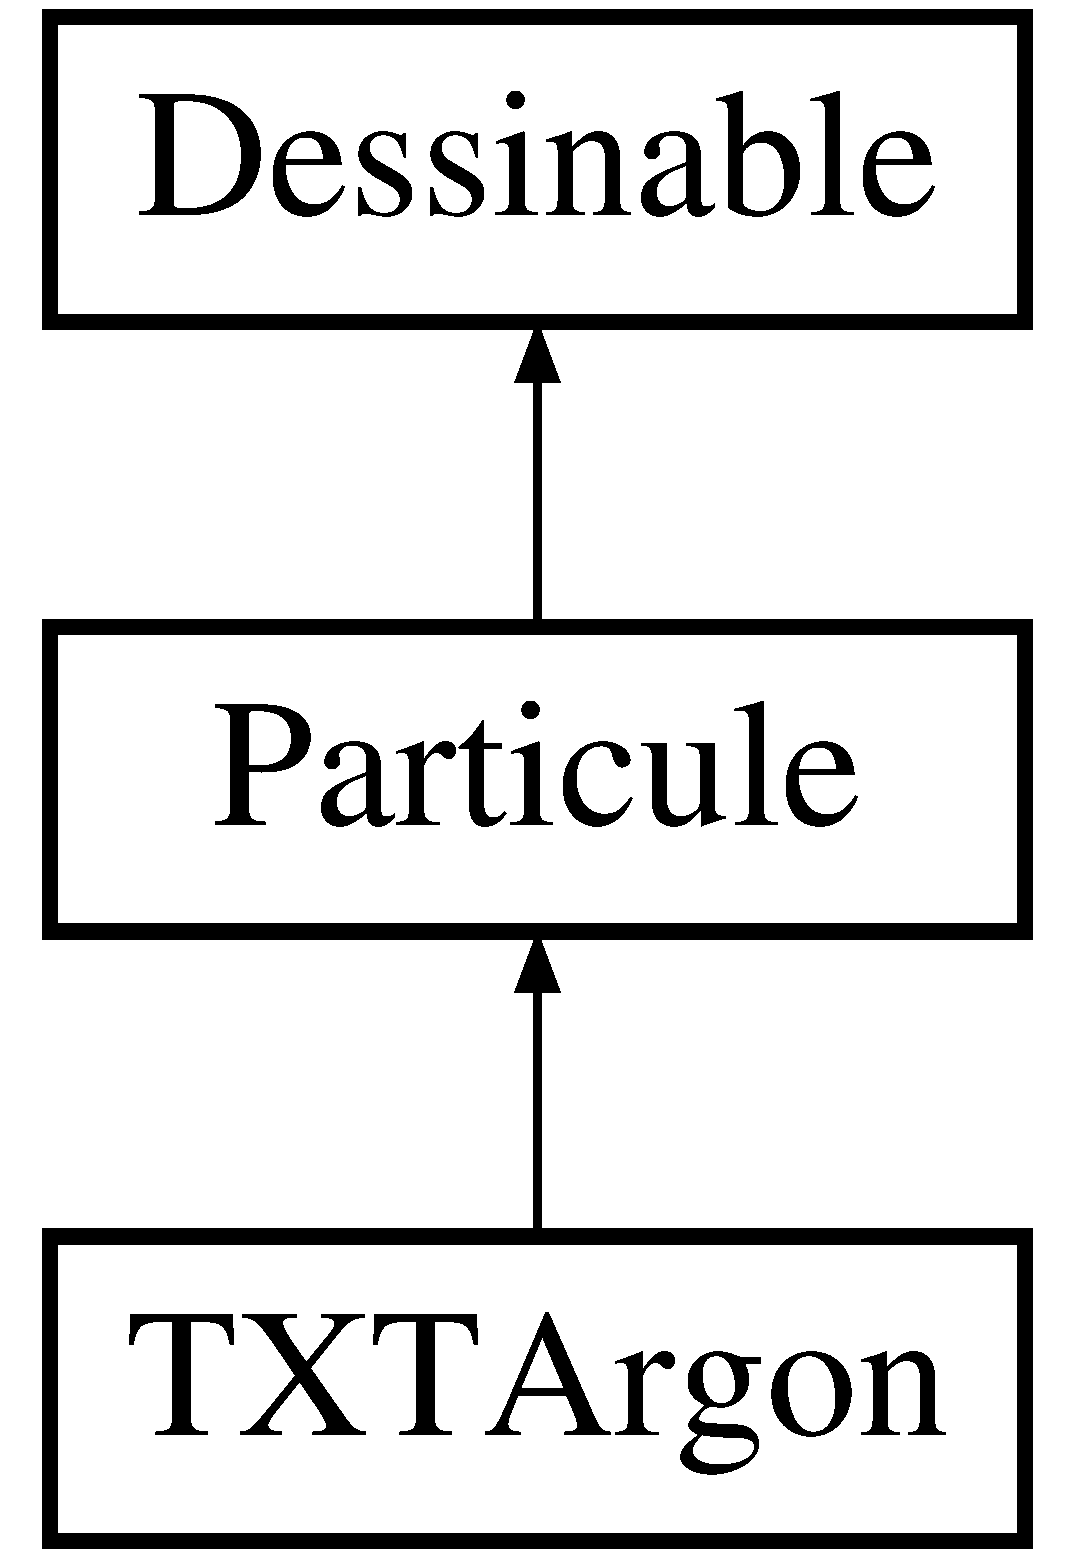
\includegraphics[height=3.000000cm]{class_t_x_t_argon}
\end{center}
\end{figure}
\subsection*{Classes}
\begin{DoxyCompactItemize}
\item 
class {\bf h}
\begin{DoxyCompactList}\small\item\em Représente des atomes d'Argon (version texte) \end{DoxyCompactList}\end{DoxyCompactItemize}
\subsection*{Fonctions membres publiques}
\begin{DoxyCompactItemize}
\item 
{\bf T\+X\+T\+Argon} ({\bf Vecteur} {\bf position}, {\bf Vecteur} {\bf vitesse})
\begin{DoxyCompactList}\small\item\em Constructeur. \end{DoxyCompactList}\item 
void {\bf dessine} () const override
\begin{DoxyCompactList}\small\item\em Redéfinition de la méthode dessine (héritée de \doxyref{Dessinable}{p.}{class_dessinable}) \end{DoxyCompactList}\end{DoxyCompactItemize}
\subsection*{Membres hérités additionnels}


\subsection{Description détaillée}


Définition à la ligne {\bf 20} du fichier {\bf T\+X\+T\+Argon.\+h}.



\subsection{Documentation des constructeurs et destructeur}
\index{T\+X\+T\+Argon@{T\+X\+T\+Argon}!T\+X\+T\+Argon@{T\+X\+T\+Argon}}
\index{T\+X\+T\+Argon@{T\+X\+T\+Argon}!T\+X\+T\+Argon@{T\+X\+T\+Argon}}
\subsubsection[{T\+X\+T\+Argon}]{\setlength{\rightskip}{0pt plus 5cm}T\+X\+T\+Argon\+::\+T\+X\+T\+Argon (
\begin{DoxyParamCaption}
\item[{{\bf Vecteur}}]{position, }
\item[{{\bf Vecteur}}]{vitesse}
\end{DoxyParamCaption}
)}\label{class_t_x_t_argon_a392a1a1f85d3dabfe3858863c90242b1}


Constructeur. 

Contructeur prenant deux paramètres de type \doxyref{Vecteur}{p.}{class_vecteur}


\begin{DoxyParams}{Paramètres}
{\em position} & \doxyref{Vecteur}{p.}{class_vecteur} correspondant à la position de la particule \\
\hline
{\em vitesse} & \doxyref{Vecteur}{p.}{class_vecteur} correspondant à la vitesse de la particule \\
\hline
\end{DoxyParams}


Définition à la ligne {\bf 17} du fichier {\bf T\+X\+T\+Argon.\+cc}.



\subsection{Documentation des fonctions membres}
\index{T\+X\+T\+Argon@{T\+X\+T\+Argon}!dessine@{dessine}}
\index{dessine@{dessine}!T\+X\+T\+Argon@{T\+X\+T\+Argon}}
\subsubsection[{dessine}]{\setlength{\rightskip}{0pt plus 5cm}void T\+X\+T\+Argon\+::dessine (
\begin{DoxyParamCaption}
{}
\end{DoxyParamCaption}
) const\hspace{0.3cm}{\ttfamily [override]}, {\ttfamily [virtual]}}\label{class_t_x_t_argon_a5ce4904e93016605cb09a9772d856b57}


Redéfinition de la méthode dessine (héritée de \doxyref{Dessinable}{p.}{class_dessinable}) 

Methode permettant de dessiner la version texte d'une particule d'Argon 

Implémente {\bf Dessinable} \doxyref{}{p.}{class_dessinable_aea37dacb2b67d6650a435d72c9a6fe79}.



Définition à la ligne {\bf 22} du fichier {\bf T\+X\+T\+Argon.\+cc}.



La documentation de cette classe a été générée à partir des fichiers suivants \+:\begin{DoxyCompactItemize}
\item 
/\+Users/burkhard/\+Dropbox/projet d'info/maximilian-\/g065/\+Simulation d'un gaz parfait/{\bf T\+X\+T\+Argon.\+h}\item 
/\+Users/burkhard/\+Dropbox/projet d'info/maximilian-\/g065/\+Simulation d'un gaz parfait/{\bf T\+X\+T\+Argon.\+cc}\end{DoxyCompactItemize}

\section{Référence de la classe T\+X\+T\+Helium}
\label{class_t_x_t_helium}\index{T\+X\+T\+Helium@{T\+X\+T\+Helium}}


{\ttfamily \#include $<$T\+X\+T\+Helium.\+h$>$}

Graphe d'héritage de T\+X\+T\+Helium\+:\begin{figure}[H]
\begin{center}
\leavevmode
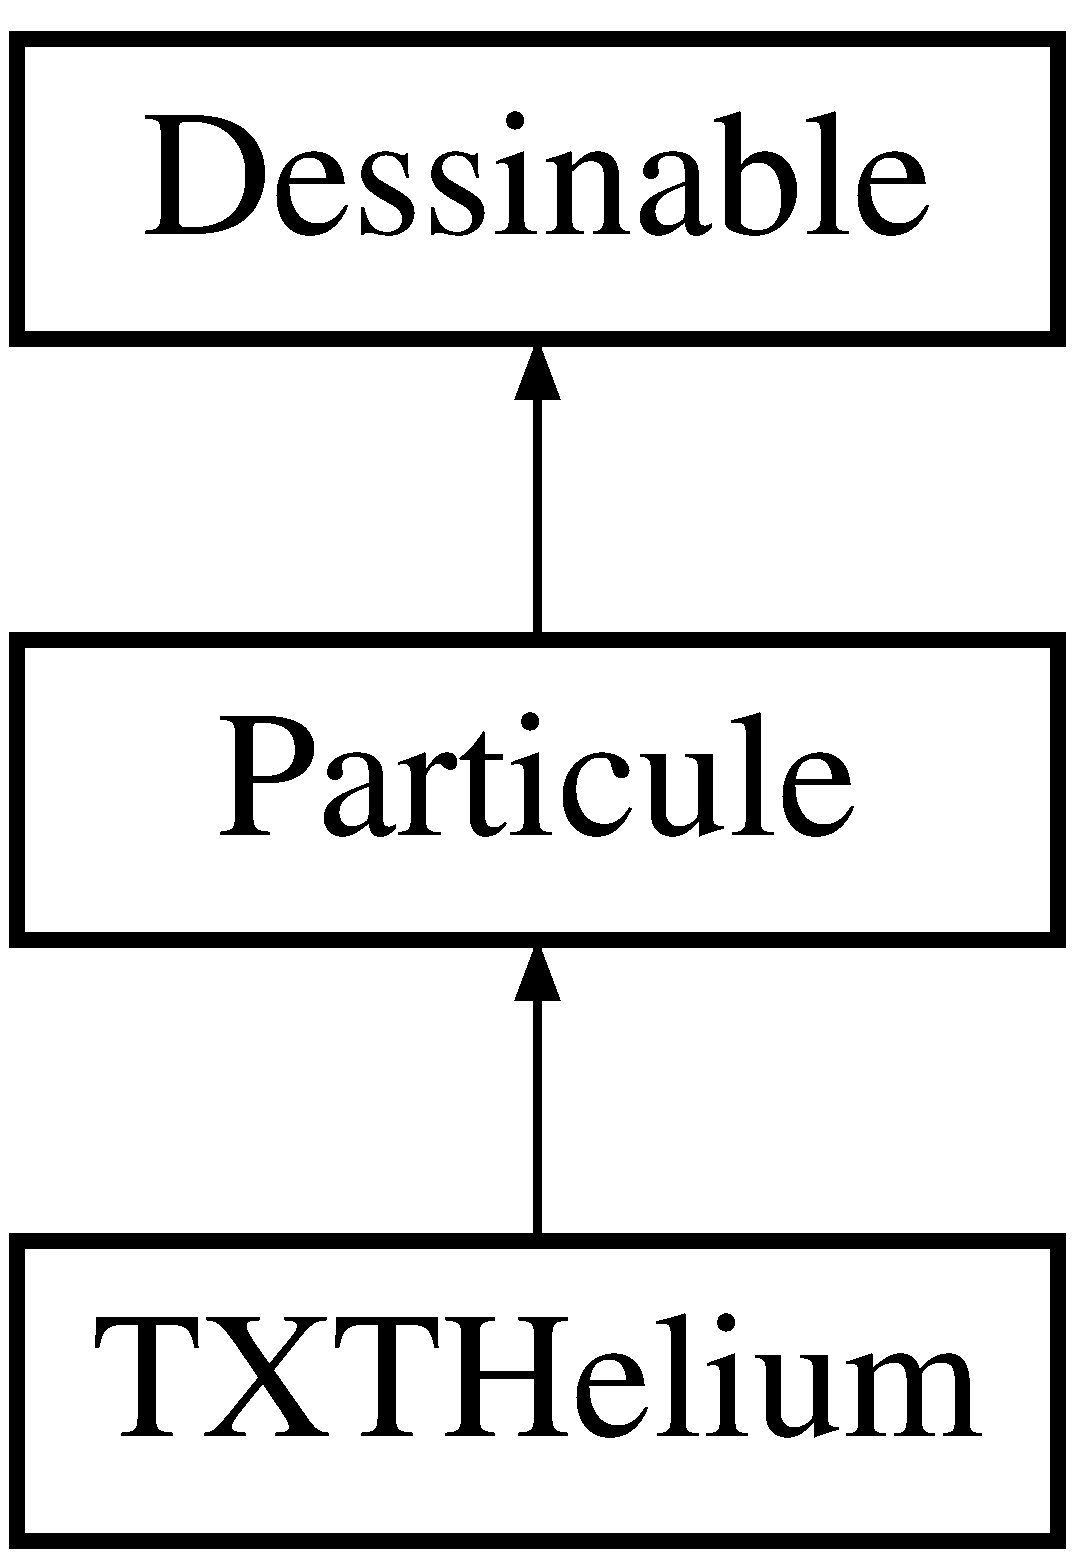
\includegraphics[height=3.000000cm]{class_t_x_t_helium}
\end{center}
\end{figure}
\subsection*{Classes}
\begin{DoxyCompactItemize}
\item 
class {\bf h}
\begin{DoxyCompactList}\small\item\em Représente des atomes d'Helium (version texte) \end{DoxyCompactList}\end{DoxyCompactItemize}
\subsection*{Fonctions membres publiques}
\begin{DoxyCompactItemize}
\item 
{\bf T\+X\+T\+Helium} ({\bf Vecteur} {\bf position}, {\bf Vecteur} {\bf vitesse})
\begin{DoxyCompactList}\small\item\em Constructeur. \end{DoxyCompactList}\item 
void {\bf dessine} () const override
\begin{DoxyCompactList}\small\item\em Redéfinition de la méthode dessine (héritée de \doxyref{Dessinable}{p.}{class_dessinable}) \end{DoxyCompactList}\end{DoxyCompactItemize}
\subsection*{Membres hérités additionnels}


\subsection{Description détaillée}


Définition à la ligne {\bf 18} du fichier {\bf T\+X\+T\+Helium.\+h}.



\subsection{Documentation des constructeurs et destructeur}
\index{T\+X\+T\+Helium@{T\+X\+T\+Helium}!T\+X\+T\+Helium@{T\+X\+T\+Helium}}
\index{T\+X\+T\+Helium@{T\+X\+T\+Helium}!T\+X\+T\+Helium@{T\+X\+T\+Helium}}
\subsubsection[{T\+X\+T\+Helium}]{\setlength{\rightskip}{0pt plus 5cm}T\+X\+T\+Helium\+::\+T\+X\+T\+Helium (
\begin{DoxyParamCaption}
\item[{{\bf Vecteur}}]{position, }
\item[{{\bf Vecteur}}]{vitesse}
\end{DoxyParamCaption}
)}\label{class_t_x_t_helium_ac66b81f8fc758ec6ffbe9882819a92d8}


Constructeur. 

Contructeur prenant deux paramètres de type \doxyref{Vecteur}{p.}{class_vecteur}


\begin{DoxyParams}{Paramètres}
{\em position} & \doxyref{Vecteur}{p.}{class_vecteur} correspondant à la position de la particule \\
\hline
{\em vitesse} & \doxyref{Vecteur}{p.}{class_vecteur} correspondant à la vitesse de la particule \\
\hline
\end{DoxyParams}


Définition à la ligne {\bf 17} du fichier {\bf T\+X\+T\+Helium.\+cc}.



\subsection{Documentation des fonctions membres}
\index{T\+X\+T\+Helium@{T\+X\+T\+Helium}!dessine@{dessine}}
\index{dessine@{dessine}!T\+X\+T\+Helium@{T\+X\+T\+Helium}}
\subsubsection[{dessine}]{\setlength{\rightskip}{0pt plus 5cm}void T\+X\+T\+Helium\+::dessine (
\begin{DoxyParamCaption}
{}
\end{DoxyParamCaption}
) const\hspace{0.3cm}{\ttfamily [override]}, {\ttfamily [virtual]}}\label{class_t_x_t_helium_a4125af216d86b3015defe5a7126d18dd}


Redéfinition de la méthode dessine (héritée de \doxyref{Dessinable}{p.}{class_dessinable}) 

Methode permettant de dessiner la version texte d'une particule d'Helium 

Implémente {\bf Dessinable} \doxyref{}{p.}{class_dessinable_aea37dacb2b67d6650a435d72c9a6fe79}.



Définition à la ligne {\bf 22} du fichier {\bf T\+X\+T\+Helium.\+cc}.



La documentation de cette classe a été générée à partir des fichiers suivants \+:\begin{DoxyCompactItemize}
\item 
/\+Users/burkhard/\+Dropbox/projet d'info/maximilian-\/g065/\+Simulation d'un gaz parfait/{\bf T\+X\+T\+Helium.\+h}\item 
/\+Users/burkhard/\+Dropbox/projet d'info/maximilian-\/g065/\+Simulation d'un gaz parfait/{\bf T\+X\+T\+Helium.\+cc}\end{DoxyCompactItemize}

\section{Référence de la classe T\+X\+T\+Neon}
\label{class_t_x_t_neon}\index{T\+X\+T\+Neon@{T\+X\+T\+Neon}}


{\ttfamily \#include $<$T\+X\+T\+Neon.\+h$>$}

Graphe d'héritage de T\+X\+T\+Neon\+:\begin{figure}[H]
\begin{center}
\leavevmode
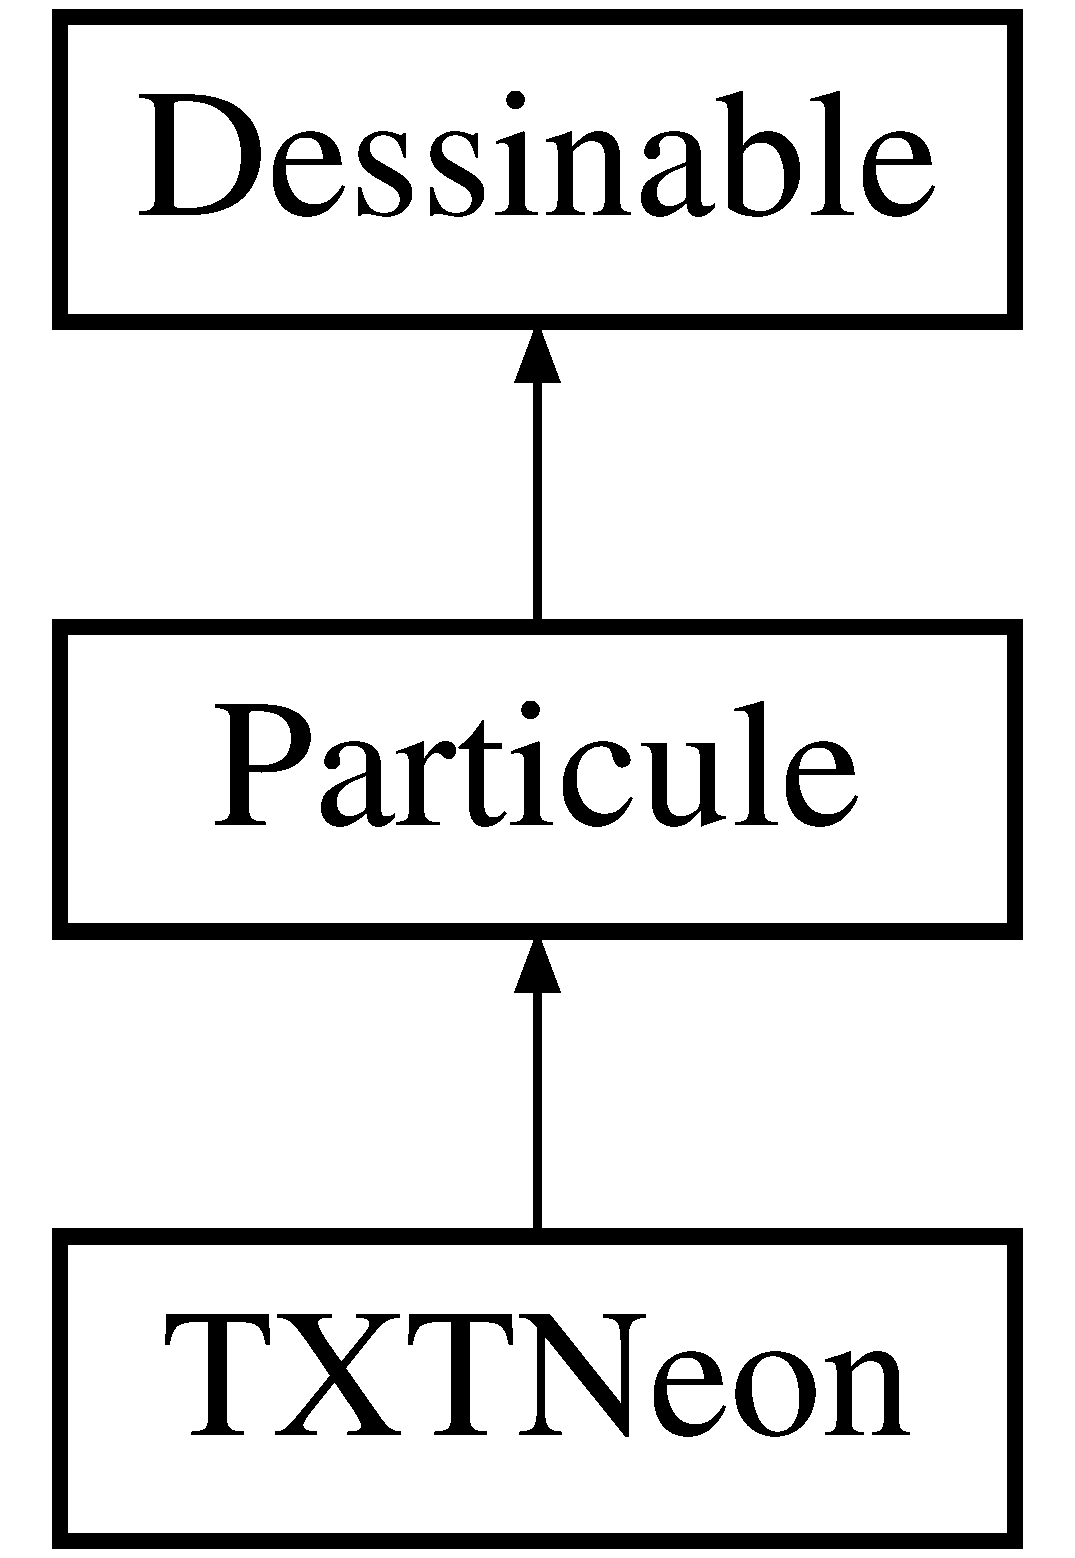
\includegraphics[height=3.000000cm]{class_t_x_t_neon}
\end{center}
\end{figure}
\subsection*{Classes}
\begin{DoxyCompactItemize}
\item 
class {\bf h}
\begin{DoxyCompactList}\small\item\em Représente des atomes de Neon (version texte) \end{DoxyCompactList}\end{DoxyCompactItemize}
\subsection*{Fonctions membres publiques}
\begin{DoxyCompactItemize}
\item 
{\bf T\+X\+T\+Neon} ({\bf Vecteur} {\bf position}, {\bf Vecteur} {\bf vitesse})
\begin{DoxyCompactList}\small\item\em Constructeur. \end{DoxyCompactList}\item 
void {\bf dessine} () const override
\begin{DoxyCompactList}\small\item\em Redéfinition de la méthode dessine (héritée de \doxyref{Dessinable}{p.}{class_dessinable}) \end{DoxyCompactList}\end{DoxyCompactItemize}
\subsection*{Membres hérités additionnels}


\subsection{Description détaillée}


Définition à la ligne {\bf 18} du fichier {\bf T\+X\+T\+Neon.\+h}.



\subsection{Documentation des constructeurs et destructeur}
\index{T\+X\+T\+Neon@{T\+X\+T\+Neon}!T\+X\+T\+Neon@{T\+X\+T\+Neon}}
\index{T\+X\+T\+Neon@{T\+X\+T\+Neon}!T\+X\+T\+Neon@{T\+X\+T\+Neon}}
\subsubsection[{T\+X\+T\+Neon}]{\setlength{\rightskip}{0pt plus 5cm}T\+X\+T\+Neon\+::\+T\+X\+T\+Neon (
\begin{DoxyParamCaption}
\item[{{\bf Vecteur}}]{position, }
\item[{{\bf Vecteur}}]{vitesse}
\end{DoxyParamCaption}
)}\label{class_t_x_t_neon_a4d4c50d098d9cd314737ad89434b421e}


Constructeur. 

Constructeur prenant deux paramètres de type \doxyref{Vecteur}{p.}{class_vecteur}


\begin{DoxyParams}{Paramètres}
{\em position} & \doxyref{Vecteur}{p.}{class_vecteur} correspondant à la position de la particule \\
\hline
{\em vitesse} & \doxyref{Vecteur}{p.}{class_vecteur} correspondant à la vitesse de la particule \\
\hline
\end{DoxyParams}


Définition à la ligne {\bf 17} du fichier {\bf T\+X\+T\+Neon.\+cc}.



\subsection{Documentation des fonctions membres}
\index{T\+X\+T\+Neon@{T\+X\+T\+Neon}!dessine@{dessine}}
\index{dessine@{dessine}!T\+X\+T\+Neon@{T\+X\+T\+Neon}}
\subsubsection[{dessine}]{\setlength{\rightskip}{0pt plus 5cm}void T\+X\+T\+Neon\+::dessine (
\begin{DoxyParamCaption}
{}
\end{DoxyParamCaption}
) const\hspace{0.3cm}{\ttfamily [override]}, {\ttfamily [virtual]}}\label{class_t_x_t_neon_a11437f76119ab389a3e47237be3a5571}


Redéfinition de la méthode dessine (héritée de \doxyref{Dessinable}{p.}{class_dessinable}) 

Methode permettant de dessiner la version texte d'une particule de Neon 

Implémente {\bf Dessinable} \doxyref{}{p.}{class_dessinable_aea37dacb2b67d6650a435d72c9a6fe79}.



Définition à la ligne {\bf 22} du fichier {\bf T\+X\+T\+Neon.\+cc}.



La documentation de cette classe a été générée à partir des fichiers suivants \+:\begin{DoxyCompactItemize}
\item 
/\+Users/burkhard/\+Dropbox/projet d'info/maximilian-\/g065/\+Simulation d'un gaz parfait/{\bf T\+X\+T\+Neon.\+h}\item 
/\+Users/burkhard/\+Dropbox/projet d'info/maximilian-\/g065/\+Simulation d'un gaz parfait/{\bf T\+X\+T\+Neon.\+cc}\end{DoxyCompactItemize}

\section{Référence de la classe Vecteur}
\label{class_vecteur}\index{Vecteur@{Vecteur}}


Prototype de la classe \doxyref{Vecteur}{p.}{class_vecteur}.  




{\ttfamily \#include $<$Vecteur.\+h$>$}

\subsection*{Fonctions membres publiques}
\begin{DoxyCompactItemize}
\item 
{\bf Vecteur} ()
\begin{DoxyCompactList}\small\item\em Constructeur sans arguments. \end{DoxyCompactList}\item 
{\bf Vecteur} (double x, double y, double z)
\begin{DoxyCompactList}\small\item\em Constructeur avec arguments qui prends les coordonnées du vecteurs. \end{DoxyCompactList}\item 
double {\bf get\+X} () const 
\begin{DoxyCompactList}\small\item\em Prototype du getters de la première coordonnée. \end{DoxyCompactList}\item 
double {\bf get\+Y} () const 
\begin{DoxyCompactList}\small\item\em Prototype du getters de la deuxième coordonnée. \end{DoxyCompactList}\item 
double {\bf get\+Z} () const 
\begin{DoxyCompactList}\small\item\em Prototype du getters de la deuxième coordonnée. \end{DoxyCompactList}\item 
bool {\bf operator==} ({\bf Vecteur} const \&) const 
\begin{DoxyCompactList}\small\item\em Prototype comparateurs ==. \end{DoxyCompactList}\item 
bool {\bf operator!=} ({\bf Vecteur} const \&v) const 
\begin{DoxyCompactList}\small\item\em Prototype comparateurs !=. \end{DoxyCompactList}\item 
{\bf Vecteur} \& {\bf operator+=} ({\bf Vecteur} const \&v1)
\begin{DoxyCompactList}\small\item\em Prototype méthodes +=. \end{DoxyCompactList}\item 
{\bf Vecteur} \& {\bf operator-\/=} ({\bf Vecteur} const \&v1)
\begin{DoxyCompactList}\small\item\em Prototype méthodes -\/=. \end{DoxyCompactList}\item 
{\bf Vecteur} \& {\bf operator$\ast$=} (double const \&scalaire)
\begin{DoxyCompactList}\small\item\em Prototype multiplication par un scalaire. \end{DoxyCompactList}\item 
double {\bf operator$\ast$} (const {\bf Vecteur} \&v1) const 
\begin{DoxyCompactList}\small\item\em Prototype produit scalaire. \end{DoxyCompactList}\item 
{\bf Vecteur} \& {\bf operator$^\wedge$=} ({\bf Vecteur} const \&v1)
\begin{DoxyCompactList}\small\item\em Prototype produit vectoriel. \end{DoxyCompactList}\item 
const {\bf Vecteur} {\bf operator-\/} ()
\begin{DoxyCompactList}\small\item\em Prototype vecteur opposé \end{DoxyCompactList}\item 
std\+::ostream \& {\bf afficher} (std\+::ostream \&sortie) const 
\begin{DoxyCompactList}\small\item\em Prototype méthode afficher. \end{DoxyCompactList}\end{DoxyCompactItemize}


\subsection{Description détaillée}
Prototype de la classe \doxyref{Vecteur}{p.}{class_vecteur}. 

Cette classe est celle qui permet de créer un vecteur, de gérer le calcul vectoriel de notre programme. 

Définition à la ligne {\bf 23} du fichier {\bf Vecteur.\+h}.



\subsection{Documentation des constructeurs et destructeur}
\index{Vecteur@{Vecteur}!Vecteur@{Vecteur}}
\index{Vecteur@{Vecteur}!Vecteur@{Vecteur}}
\subsubsection[{Vecteur}]{\setlength{\rightskip}{0pt plus 5cm}Vecteur\+::\+Vecteur (
\begin{DoxyParamCaption}
{}
\end{DoxyParamCaption}
)}\label{class_vecteur_a8227543ef6aadc8f9fbbc93de68af43b}


Constructeur sans arguments. 

Constructeur de la classe \doxyref{Vecteur}{p.}{class_vecteur} sans arguments 

Définition à la ligne {\bf 20} du fichier {\bf Vecteur.\+cc}.

\index{Vecteur@{Vecteur}!Vecteur@{Vecteur}}
\index{Vecteur@{Vecteur}!Vecteur@{Vecteur}}
\subsubsection[{Vecteur}]{\setlength{\rightskip}{0pt plus 5cm}Vecteur\+::\+Vecteur (
\begin{DoxyParamCaption}
\item[{double}]{x, }
\item[{double}]{y, }
\item[{double}]{z}
\end{DoxyParamCaption}
)}\label{class_vecteur_a74467c37b0023c84ee3f64d09348a660}


Constructeur avec arguments qui prends les coordonnées du vecteurs. 

Constructeur de la classe \doxyref{Vecteur}{p.}{class_vecteur} avec trois arguements de type double


\begin{DoxyParams}{Paramètres}
{\em x} & \+: première coordonnée x \\
\hline
{\em y} & \+: deuxième coordonnée y \\
\hline
{\em z} & \+: troisième coordonnée z \\
\hline
\end{DoxyParams}


Définition à la ligne {\bf 30} du fichier {\bf Vecteur.\+cc}.



\subsection{Documentation des fonctions membres}
\index{Vecteur@{Vecteur}!afficher@{afficher}}
\index{afficher@{afficher}!Vecteur@{Vecteur}}
\subsubsection[{afficher}]{\setlength{\rightskip}{0pt plus 5cm}ostream \& Vecteur\+::afficher (
\begin{DoxyParamCaption}
\item[{std\+::ostream \&}]{sortie}
\end{DoxyParamCaption}
) const}\label{class_vecteur_ac0d4143f79e766d00a55ba86f7ba44fa}


Prototype méthode afficher. 


\begin{DoxyParams}{Paramètres}
{\em ostream\&} & sortie \+: permet de choisir le flot de sortie \\
\hline
\end{DoxyParams}
\begin{DoxyReturn}{Renvoie}
un ostream\& pour pouvoir faire des \char`\"{}appels multiples\char`\"{} 
\end{DoxyReturn}


Définition à la ligne {\bf 172} du fichier {\bf Vecteur.\+cc}.

\index{Vecteur@{Vecteur}!get\+X@{get\+X}}
\index{get\+X@{get\+X}!Vecteur@{Vecteur}}
\subsubsection[{get\+X}]{\setlength{\rightskip}{0pt plus 5cm}double Vecteur\+::get\+X (
\begin{DoxyParamCaption}
{}
\end{DoxyParamCaption}
) const}\label{class_vecteur_a42f7a7f1dc44e088c278d3b3363c5a33}


Prototype du getters de la première coordonnée. 

Methode qui permet de retourner les attributs privés du \doxyref{Vecteur}{p.}{class_vecteur}

\begin{DoxyReturn}{Renvoie}
la coordonée en x 
\end{DoxyReturn}


Définition à la ligne {\bf 41} du fichier {\bf Vecteur.\+cc}.

\index{Vecteur@{Vecteur}!get\+Y@{get\+Y}}
\index{get\+Y@{get\+Y}!Vecteur@{Vecteur}}
\subsubsection[{get\+Y}]{\setlength{\rightskip}{0pt plus 5cm}double Vecteur\+::get\+Y (
\begin{DoxyParamCaption}
{}
\end{DoxyParamCaption}
) const}\label{class_vecteur_a323d689fb951261b557ea65b10af3893}


Prototype du getters de la deuxième coordonnée. 

Methode qui permet de retourner les attributs privés du \doxyref{Vecteur}{p.}{class_vecteur}

\begin{DoxyReturn}{Renvoie}
la coordonée en y 
\end{DoxyReturn}


Définition à la ligne {\bf 50} du fichier {\bf Vecteur.\+cc}.

\index{Vecteur@{Vecteur}!get\+Z@{get\+Z}}
\index{get\+Z@{get\+Z}!Vecteur@{Vecteur}}
\subsubsection[{get\+Z}]{\setlength{\rightskip}{0pt plus 5cm}double Vecteur\+::get\+Z (
\begin{DoxyParamCaption}
{}
\end{DoxyParamCaption}
) const}\label{class_vecteur_a9ceff1802cdc94554cb8556fb9d94058}


Prototype du getters de la deuxième coordonnée. 

Methode qui permet de retourner les attributs privés du \doxyref{Vecteur}{p.}{class_vecteur}

\begin{DoxyReturn}{Renvoie}
la coordonée en z 
\end{DoxyReturn}


Définition à la ligne {\bf 59} du fichier {\bf Vecteur.\+cc}.

\index{Vecteur@{Vecteur}!operator"!=@{operator"!=}}
\index{operator"!=@{operator"!=}!Vecteur@{Vecteur}}
\subsubsection[{operator"!=}]{\setlength{\rightskip}{0pt plus 5cm}bool Vecteur\+::operator!= (
\begin{DoxyParamCaption}
\item[{{\bf Vecteur} const \&}]{v}
\end{DoxyParamCaption}
) const}\label{class_vecteur_a07fd3198ced9a6f4b746e1d406a5796f}


Prototype comparateurs !=. 


\begin{DoxyParams}{Paramètres}
{\em \doxyref{Vecteur}{p.}{class_vecteur}} & const\& v \+: permet de comparer la différence au deuxième vecteur \\
\hline
\end{DoxyParams}
\begin{DoxyReturn}{Renvoie}
true si le vecteur est différents de v sinon il retourne false 
\end{DoxyReturn}


Définition à la ligne {\bf 84} du fichier {\bf Vecteur.\+cc}.

\index{Vecteur@{Vecteur}!operator$\ast$@{operator$\ast$}}
\index{operator$\ast$@{operator$\ast$}!Vecteur@{Vecteur}}
\subsubsection[{operator$\ast$}]{\setlength{\rightskip}{0pt plus 5cm}double Vecteur\+::operator$\ast$ (
\begin{DoxyParamCaption}
\item[{const {\bf Vecteur} \&}]{v1}
\end{DoxyParamCaption}
) const}\label{class_vecteur_a5ee19aab50156659ac236029316209ea}


Prototype produit scalaire. 

fait le produit scalaire de deux vecteurs


\begin{DoxyParams}{Paramètres}
{\em \doxyref{Vecteur}{p.}{class_vecteur}} & const\& v1 \+: permet de calculer le produit scalaire \\
\hline
\end{DoxyParams}
\begin{DoxyReturn}{Renvoie}
un double (nombre réel) qui est le produit scalaire 
\end{DoxyReturn}


Définition à la ligne {\bf 163} du fichier {\bf Vecteur.\+cc}.

\index{Vecteur@{Vecteur}!operator$\ast$=@{operator$\ast$=}}
\index{operator$\ast$=@{operator$\ast$=}!Vecteur@{Vecteur}}
\subsubsection[{operator$\ast$=}]{\setlength{\rightskip}{0pt plus 5cm}{\bf Vecteur} \& Vecteur\+::operator$\ast$= (
\begin{DoxyParamCaption}
\item[{double const \&}]{scalaire}
\end{DoxyParamCaption}
)}\label{class_vecteur_a46ab3e3e8a9baf796d7cce7ec6f56c74}


Prototype multiplication par un scalaire. 

permet de multiplier le vecteur à un nombre scalaire et de l'enregistrer dans le vecteur appelant


\begin{DoxyParams}{Paramètres}
{\em double} & const\& scalaire \+: le nombre par lequel on va multiplier \\
\hline
\end{DoxyParams}
\begin{DoxyReturn}{Renvoie}
le vecteur appelant 
\end{DoxyReturn}


Définition à la ligne {\bf 133} du fichier {\bf Vecteur.\+cc}.

\index{Vecteur@{Vecteur}!operator+=@{operator+=}}
\index{operator+=@{operator+=}!Vecteur@{Vecteur}}
\subsubsection[{operator+=}]{\setlength{\rightskip}{0pt plus 5cm}{\bf Vecteur} \& Vecteur\+::operator+= (
\begin{DoxyParamCaption}
\item[{{\bf Vecteur} const \&}]{v1}
\end{DoxyParamCaption}
)}\label{class_vecteur_ae5976277e40ef72d4bd9e206010ebae9}


Prototype méthodes +=. 

aditionne le vecteur appelant au vecteur v en paramètre et l'enregistre dans l'objet appelant


\begin{DoxyParams}{Paramètres}
{\em \doxyref{Vecteur}{p.}{class_vecteur}} & const\& v \+: permet d'additionner le deuxième vecteur \\
\hline
\end{DoxyParams}
\begin{DoxyReturn}{Renvoie}
le vecteur appelant 
\end{DoxyReturn}


Définition à la ligne {\bf 95} du fichier {\bf Vecteur.\+cc}.

\index{Vecteur@{Vecteur}!operator-\/@{operator-\/}}
\index{operator-\/@{operator-\/}!Vecteur@{Vecteur}}
\subsubsection[{operator-\/}]{\setlength{\rightskip}{0pt plus 5cm}const {\bf Vecteur} Vecteur\+::operator-\/ (
\begin{DoxyParamCaption}
{}
\end{DoxyParamCaption}
)}\label{class_vecteur_a57540f656ae1f3e6ee9ff22cd37ef081}


Prototype vecteur opposé 

fait l'opposer du vecteur appelant

\begin{DoxyReturn}{Renvoie}
le vecteur appelant opposé 
\end{DoxyReturn}


Définition à la ligne {\bf 122} du fichier {\bf Vecteur.\+cc}.

\index{Vecteur@{Vecteur}!operator-\/=@{operator-\/=}}
\index{operator-\/=@{operator-\/=}!Vecteur@{Vecteur}}
\subsubsection[{operator-\/=}]{\setlength{\rightskip}{0pt plus 5cm}{\bf Vecteur} \& Vecteur\+::operator-\/= (
\begin{DoxyParamCaption}
\item[{{\bf Vecteur} const \&}]{v1}
\end{DoxyParamCaption}
)}\label{class_vecteur_a2e64b160a4df2b937b98a4f8341c0bd7}


Prototype méthodes -\/=. 

soustrait le vecteur appelant au vecteur v en paramètre et l'enregistre dans l'objet appelant


\begin{DoxyParams}{Paramètres}
{\em \doxyref{Vecteur}{p.}{class_vecteur}} & const\& v \+: permet de soustraire le deuxième vecteur \\
\hline
\end{DoxyParams}
\begin{DoxyReturn}{Renvoie}
le vecteur appelant 
\end{DoxyReturn}


Définition à la ligne {\bf 109} du fichier {\bf Vecteur.\+cc}.

\index{Vecteur@{Vecteur}!operator==@{operator==}}
\index{operator==@{operator==}!Vecteur@{Vecteur}}
\subsubsection[{operator==}]{\setlength{\rightskip}{0pt plus 5cm}bool Vecteur\+::operator== (
\begin{DoxyParamCaption}
\item[{{\bf Vecteur} const \&}]{v}
\end{DoxyParamCaption}
) const}\label{class_vecteur_a9201e305c2028d0d596c24327560f8ca}


Prototype comparateurs ==. 


\begin{DoxyParams}{Paramètres}
{\em \doxyref{Vecteur}{p.}{class_vecteur}} & const\& v \+: permet de comparer au deuxième vecteur \\
\hline
\end{DoxyParams}
\begin{DoxyReturn}{Renvoie}
true s'il sont égale et false sinon 
\end{DoxyReturn}


Définition à la ligne {\bf 68} du fichier {\bf Vecteur.\+cc}.

\index{Vecteur@{Vecteur}!operator$^\wedge$=@{operator$^\wedge$=}}
\index{operator$^\wedge$=@{operator$^\wedge$=}!Vecteur@{Vecteur}}
\subsubsection[{operator$^\wedge$=}]{\setlength{\rightskip}{0pt plus 5cm}{\bf Vecteur} \& Vecteur\+::operator$^\wedge$= (
\begin{DoxyParamCaption}
\item[{{\bf Vecteur} const \&}]{v1}
\end{DoxyParamCaption}
)}\label{class_vecteur_a70e7d84a9e5bb9fe9ef06b6697324294}


Prototype produit vectoriel. 

permet de faire le produit vectoriel avec le vecteur en paramètre et l'enregistrer dans le vecteur appelant le calcul ce fait comme le produit vectoriel usuels


\begin{DoxyParams}{Paramètres}
{\em \doxyref{Vecteur}{p.}{class_vecteur}} & const\& v1 \+: permet de calculer le produit vectoriel avec le deuxième vecteur \\
\hline
\end{DoxyParams}
\begin{DoxyReturn}{Renvoie}
le vecteur appelant qui est le produit vectoriel des deux vecteurs 
\end{DoxyReturn}


Définition à la ligne {\bf 148} du fichier {\bf Vecteur.\+cc}.



La documentation de cette classe a été générée à partir des fichiers suivants \+:\begin{DoxyCompactItemize}
\item 
/\+Users/burkhard/\+Dropbox/projet d'info/maximilian-\/g065/\+Simulation d'un gaz parfait/{\bf Vecteur.\+h}\item 
/\+Users/burkhard/\+Dropbox/projet d'info/maximilian-\/g065/\+Simulation d'un gaz parfait/{\bf Vecteur.\+cc}\end{DoxyCompactItemize}

\section{Référence de la classe Vue\+\_\+\+Open\+G\+L}
\label{class_vue___open_g_l}\index{Vue\+\_\+\+Open\+G\+L@{Vue\+\_\+\+Open\+G\+L}}


Prototype de la classe \doxyref{Vue\+\_\+\+Open\+G\+L}{p.}{class_vue___open_g_l}.  




{\ttfamily \#include $<$Vue\+\_\+\+Open\+G\+L.\+h$>$}

Graphe d'héritage de Vue\+\_\+\+Open\+G\+L\+:\begin{figure}[H]
\begin{center}
\leavevmode
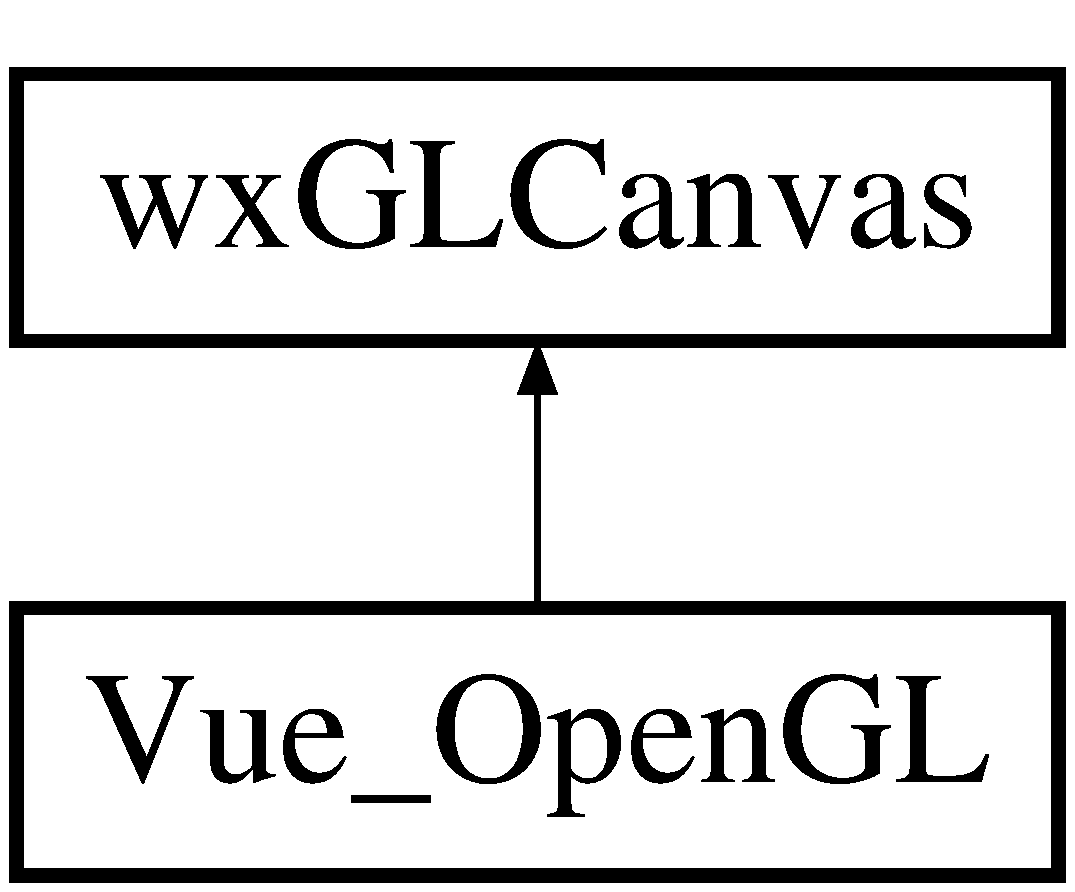
\includegraphics[height=2.000000cm]{class_vue___open_g_l}
\end{center}
\end{figure}
\subsection*{Fonctions membres publiques}
\begin{DoxyCompactItemize}
\item 
{\bf Vue\+\_\+\+Open\+G\+L} (wx\+Window $\ast$parent, wx\+Size const \&taille=wx\+Default\+Size, wx\+Point const \&position=wx\+Default\+Position)
\begin{DoxyCompactList}\small\item\em constructeur \doxyref{Vue\+\_\+\+Open\+G\+L}{p.}{class_vue___open_g_l} \end{DoxyCompactList}\item 
{\bf Vue\+\_\+\+Open\+G\+L} (wx\+Window $\ast$parent, bool reglage, wx\+Size const \&taille=wx\+Default\+Size, wx\+Point const \&position=wx\+Default\+Position)
\begin{DoxyCompactList}\small\item\em constructeur \doxyref{Vue\+\_\+\+Open\+G\+L}{p.}{class_vue___open_g_l} \end{DoxyCompactList}\item 
virtual {\bf $\sim$\+Vue\+\_\+\+Open\+G\+L} ()
\begin{DoxyCompactList}\small\item\em Destructeur. \end{DoxyCompactList}\item 
void {\bf Init\+Open\+G\+L} ()
\begin{DoxyCompactList}\small\item\em prototype public de la méthode qui va appeler evolue de systeme \end{DoxyCompactList}\end{DoxyCompactItemize}
\subsection*{Fonctions membres protégées}
\begin{DoxyCompactItemize}
\item 
void {\bf dessine} (wx\+Paint\+Event \&evenement)
\begin{DoxyCompactList}\small\item\em prototype de la méthode dessine \end{DoxyCompactList}\item 
void {\bf On\+Size} (wx\+Size\+Event \&evenement)
\item 
void {\bf On\+Key\+Down} (wx\+Key\+Event \&evenement)
\begin{DoxyCompactList}\small\item\em prototype de la méthode qui gère les événements du claviers \end{DoxyCompactList}\item 
void {\bf On\+Enter\+Window} (wx\+Mouse\+Event \&evenement)
\begin{DoxyCompactList}\small\item\em prototype de la méthode qui gères les éveénement de la souris \end{DoxyCompactList}\item 
void {\bf On\+Timer} (wx\+Timer\+Event \&event)
\begin{DoxyCompactList}\small\item\em prototype de la méthode du Timer qui va appeler la méthode évolue du système \end{DoxyCompactList}\item 
void {\bf Rotate\+Theta} (G\+Ldouble deg)
\begin{DoxyCompactList}\small\item\em prototype de la méthode qui fait la rotation de l'angle theta pour la caméra \end{DoxyCompactList}\item 
void {\bf Rotate\+Phi} (G\+Ldouble deg)
\begin{DoxyCompactList}\small\item\em prototype de la méthode qui fait la rotation de l'angle phi pour la caméra \end{DoxyCompactList}\item 
void {\bf deplace} (double dr)
\begin{DoxyCompactList}\small\item\em prototype de la méthode qui fait le déplacement de la caméra \end{DoxyCompactList}\end{DoxyCompactItemize}


\subsection{Description détaillée}
Prototype de la classe \doxyref{Vue\+\_\+\+Open\+G\+L}{p.}{class_vue___open_g_l}. 

Cette classe est ce qui remplira la fenêtre et qui gère les animations dans celle-\/ci comme notre simulation du gaz parfait. Elle est écrite avec du C++ et de l'Open\+G\+L. representant la partie de l'Open\+G\+L qui va instancier presque toutes les parties de notre simulation 

Définition à la ligne {\bf 30} du fichier {\bf Vue\+\_\+\+Open\+G\+L.\+h}.



\subsection{Documentation des constructeurs et destructeur}
\index{Vue\+\_\+\+Open\+G\+L@{Vue\+\_\+\+Open\+G\+L}!Vue\+\_\+\+Open\+G\+L@{Vue\+\_\+\+Open\+G\+L}}
\index{Vue\+\_\+\+Open\+G\+L@{Vue\+\_\+\+Open\+G\+L}!Vue\+\_\+\+Open\+G\+L@{Vue\+\_\+\+Open\+G\+L}}
\subsubsection[{Vue\+\_\+\+Open\+G\+L}]{\setlength{\rightskip}{0pt plus 5cm}Vue\+\_\+\+Open\+G\+L\+::\+Vue\+\_\+\+Open\+G\+L (
\begin{DoxyParamCaption}
\item[{wx\+Window $\ast$}]{parent, }
\item[{wx\+Size const \&}]{taille = {\ttfamily wxDefaultSize}, }
\item[{wx\+Point const \&}]{position = {\ttfamily wxDefaultPosition}}
\end{DoxyParamCaption}
)}\label{class_vue___open_g_l_a8b6c60ae47c2b0d988f39ea788aa4ed4}


constructeur \doxyref{Vue\+\_\+\+Open\+G\+L}{p.}{class_vue___open_g_l} 

Constructeur.

Constructeur de la Vue\+\_\+\+Oen\+G\+L qui initialise le système, le timer, la position de la caméra au départ 

Définition à la ligne {\bf 43} du fichier {\bf Vue\+\_\+\+Open\+G\+L.\+cc}.

\index{Vue\+\_\+\+Open\+G\+L@{Vue\+\_\+\+Open\+G\+L}!Vue\+\_\+\+Open\+G\+L@{Vue\+\_\+\+Open\+G\+L}}
\index{Vue\+\_\+\+Open\+G\+L@{Vue\+\_\+\+Open\+G\+L}!Vue\+\_\+\+Open\+G\+L@{Vue\+\_\+\+Open\+G\+L}}
\subsubsection[{Vue\+\_\+\+Open\+G\+L}]{\setlength{\rightskip}{0pt plus 5cm}Vue\+\_\+\+Open\+G\+L\+::\+Vue\+\_\+\+Open\+G\+L (
\begin{DoxyParamCaption}
\item[{wx\+Window $\ast$}]{parent, }
\item[{bool}]{reglage, }
\item[{wx\+Size const \&}]{taille = {\ttfamily wxDefaultSize}, }
\item[{wx\+Point const \&}]{position = {\ttfamily wxDefaultPosition}}
\end{DoxyParamCaption}
)}\label{class_vue___open_g_l_a89f69951ff60193ed93e0653c268fcc1}


constructeur \doxyref{Vue\+\_\+\+Open\+G\+L}{p.}{class_vue___open_g_l} 

Constructeur.

Constructeur de la Vue\+\_\+\+Oen\+G\+L qui initialise le système, le timer, la position de la caméra au départ 

Définition à la ligne {\bf 61} du fichier {\bf Vue\+\_\+\+Open\+G\+L.\+cc}.

\index{Vue\+\_\+\+Open\+G\+L@{Vue\+\_\+\+Open\+G\+L}!````~Vue\+\_\+\+Open\+G\+L@{$\sim$\+Vue\+\_\+\+Open\+G\+L}}
\index{````~Vue\+\_\+\+Open\+G\+L@{$\sim$\+Vue\+\_\+\+Open\+G\+L}!Vue\+\_\+\+Open\+G\+L@{Vue\+\_\+\+Open\+G\+L}}
\subsubsection[{$\sim$\+Vue\+\_\+\+Open\+G\+L}]{\setlength{\rightskip}{0pt plus 5cm}virtual Vue\+\_\+\+Open\+G\+L\+::$\sim$\+Vue\+\_\+\+Open\+G\+L (
\begin{DoxyParamCaption}
{}
\end{DoxyParamCaption}
)\hspace{0.3cm}{\ttfamily [inline]}, {\ttfamily [virtual]}}\label{class_vue___open_g_l_a6a2ba551a35f5ac35a3ee1f78b9c00d1}


Destructeur. 

Destructeur de la classe \doxyref{Vue\+\_\+\+Open\+G\+L}{p.}{class_vue___open_g_l} 

Définition à la ligne {\bf 51} du fichier {\bf Vue\+\_\+\+Open\+G\+L.\+h}.



\subsection{Documentation des fonctions membres}
\index{Vue\+\_\+\+Open\+G\+L@{Vue\+\_\+\+Open\+G\+L}!deplace@{deplace}}
\index{deplace@{deplace}!Vue\+\_\+\+Open\+G\+L@{Vue\+\_\+\+Open\+G\+L}}
\subsubsection[{deplace}]{\setlength{\rightskip}{0pt plus 5cm}void Vue\+\_\+\+Open\+G\+L\+::deplace (
\begin{DoxyParamCaption}
\item[{double}]{dr}
\end{DoxyParamCaption}
)\hspace{0.3cm}{\ttfamily [protected]}}\label{class_vue___open_g_l_afdcf7b3ea31efc02c773aba58eb6617c}


prototype de la méthode qui fait le déplacement de la caméra 



Définition à la ligne {\bf 205} du fichier {\bf Vue\+\_\+\+Open\+G\+L.\+cc}.

\index{Vue\+\_\+\+Open\+G\+L@{Vue\+\_\+\+Open\+G\+L}!dessine@{dessine}}
\index{dessine@{dessine}!Vue\+\_\+\+Open\+G\+L@{Vue\+\_\+\+Open\+G\+L}}
\subsubsection[{dessine}]{\setlength{\rightskip}{0pt plus 5cm}void Vue\+\_\+\+Open\+G\+L\+::dessine (
\begin{DoxyParamCaption}
\item[{wx\+Paint\+Event \&}]{evenement}
\end{DoxyParamCaption}
)\hspace{0.3cm}{\ttfamily [protected]}}\label{class_vue___open_g_l_a73b8426ef156d44965e29842a7cc91ed}


prototype de la méthode dessine 



Définition à la ligne {\bf 74} du fichier {\bf Vue\+\_\+\+Open\+G\+L.\+cc}.

\index{Vue\+\_\+\+Open\+G\+L@{Vue\+\_\+\+Open\+G\+L}!Init\+Open\+G\+L@{Init\+Open\+G\+L}}
\index{Init\+Open\+G\+L@{Init\+Open\+G\+L}!Vue\+\_\+\+Open\+G\+L@{Vue\+\_\+\+Open\+G\+L}}
\subsubsection[{Init\+Open\+G\+L}]{\setlength{\rightskip}{0pt plus 5cm}void Vue\+\_\+\+Open\+G\+L\+::\+Init\+Open\+G\+L (
\begin{DoxyParamCaption}
{}
\end{DoxyParamCaption}
)}\label{class_vue___open_g_l_a6ed4a73bf485eeb80d1ffbd209eb523f}


prototype public de la méthode qui va appeler evolue de systeme 



Définition à la ligne {\bf 213} du fichier {\bf Vue\+\_\+\+Open\+G\+L.\+cc}.

\index{Vue\+\_\+\+Open\+G\+L@{Vue\+\_\+\+Open\+G\+L}!On\+Enter\+Window@{On\+Enter\+Window}}
\index{On\+Enter\+Window@{On\+Enter\+Window}!Vue\+\_\+\+Open\+G\+L@{Vue\+\_\+\+Open\+G\+L}}
\subsubsection[{On\+Enter\+Window}]{\setlength{\rightskip}{0pt plus 5cm}void Vue\+\_\+\+Open\+G\+L\+::\+On\+Enter\+Window (
\begin{DoxyParamCaption}
\item[{wx\+Mouse\+Event \&}]{evenement}
\end{DoxyParamCaption}
)\hspace{0.3cm}{\ttfamily [inline]}, {\ttfamily [protected]}}\label{class_vue___open_g_l_a49651d519ec8909490a89a688b79a524}


prototype de la méthode qui gères les éveénement de la souris 



Définition à la ligne {\bf 63} du fichier {\bf Vue\+\_\+\+Open\+G\+L.\+h}.

\index{Vue\+\_\+\+Open\+G\+L@{Vue\+\_\+\+Open\+G\+L}!On\+Key\+Down@{On\+Key\+Down}}
\index{On\+Key\+Down@{On\+Key\+Down}!Vue\+\_\+\+Open\+G\+L@{Vue\+\_\+\+Open\+G\+L}}
\subsubsection[{On\+Key\+Down}]{\setlength{\rightskip}{0pt plus 5cm}void Vue\+\_\+\+Open\+G\+L\+::\+On\+Key\+Down (
\begin{DoxyParamCaption}
\item[{wx\+Key\+Event \&}]{evenement}
\end{DoxyParamCaption}
)\hspace{0.3cm}{\ttfamily [protected]}}\label{class_vue___open_g_l_aa92d4dcdce7b7afbc6507d8f8cead104}


prototype de la méthode qui gère les événements du claviers 



Définition à la ligne {\bf 119} du fichier {\bf Vue\+\_\+\+Open\+G\+L.\+cc}.

\index{Vue\+\_\+\+Open\+G\+L@{Vue\+\_\+\+Open\+G\+L}!On\+Size@{On\+Size}}
\index{On\+Size@{On\+Size}!Vue\+\_\+\+Open\+G\+L@{Vue\+\_\+\+Open\+G\+L}}
\subsubsection[{On\+Size}]{\setlength{\rightskip}{0pt plus 5cm}void Vue\+\_\+\+Open\+G\+L\+::\+On\+Size (
\begin{DoxyParamCaption}
\item[{wx\+Size\+Event \&}]{evenement}
\end{DoxyParamCaption}
)\hspace{0.3cm}{\ttfamily [protected]}}\label{class_vue___open_g_l_a8ba5bfc69bc8719ae9024d603de3dd55}


Définition à la ligne {\bf 104} du fichier {\bf Vue\+\_\+\+Open\+G\+L.\+cc}.

\index{Vue\+\_\+\+Open\+G\+L@{Vue\+\_\+\+Open\+G\+L}!On\+Timer@{On\+Timer}}
\index{On\+Timer@{On\+Timer}!Vue\+\_\+\+Open\+G\+L@{Vue\+\_\+\+Open\+G\+L}}
\subsubsection[{On\+Timer}]{\setlength{\rightskip}{0pt plus 5cm}void Vue\+\_\+\+Open\+G\+L\+::\+On\+Timer (
\begin{DoxyParamCaption}
\item[{wx\+Timer\+Event \&}]{event}
\end{DoxyParamCaption}
)\hspace{0.3cm}{\ttfamily [protected]}}\label{class_vue___open_g_l_a115fe5326875d273202e9917c45b2cf5}


prototype de la méthode du Timer qui va appeler la méthode évolue du système 



Définition à la ligne {\bf 239} du fichier {\bf Vue\+\_\+\+Open\+G\+L.\+cc}.

\index{Vue\+\_\+\+Open\+G\+L@{Vue\+\_\+\+Open\+G\+L}!Rotate\+Phi@{Rotate\+Phi}}
\index{Rotate\+Phi@{Rotate\+Phi}!Vue\+\_\+\+Open\+G\+L@{Vue\+\_\+\+Open\+G\+L}}
\subsubsection[{Rotate\+Phi}]{\setlength{\rightskip}{0pt plus 5cm}void Vue\+\_\+\+Open\+G\+L\+::\+Rotate\+Phi (
\begin{DoxyParamCaption}
\item[{G\+Ldouble}]{deg}
\end{DoxyParamCaption}
)\hspace{0.3cm}{\ttfamily [protected]}}\label{class_vue___open_g_l_a1da1dad7d2da5a1ef3f834cd4ac5a35e}


prototype de la méthode qui fait la rotation de l'angle phi pour la caméra 



Définition à la ligne {\bf 197} du fichier {\bf Vue\+\_\+\+Open\+G\+L.\+cc}.

\index{Vue\+\_\+\+Open\+G\+L@{Vue\+\_\+\+Open\+G\+L}!Rotate\+Theta@{Rotate\+Theta}}
\index{Rotate\+Theta@{Rotate\+Theta}!Vue\+\_\+\+Open\+G\+L@{Vue\+\_\+\+Open\+G\+L}}
\subsubsection[{Rotate\+Theta}]{\setlength{\rightskip}{0pt plus 5cm}void Vue\+\_\+\+Open\+G\+L\+::\+Rotate\+Theta (
\begin{DoxyParamCaption}
\item[{G\+Ldouble}]{deg}
\end{DoxyParamCaption}
)\hspace{0.3cm}{\ttfamily [protected]}}\label{class_vue___open_g_l_a088c8fb20c9ba9c25cd5aa5eaeac4e5c}


prototype de la méthode qui fait la rotation de l'angle theta pour la caméra 



Définition à la ligne {\bf 189} du fichier {\bf Vue\+\_\+\+Open\+G\+L.\+cc}.



La documentation de cette classe a été générée à partir des fichiers suivants \+:\begin{DoxyCompactItemize}
\item 
/\+Users/burkhard/\+Dropbox/projet d'info/maximilian-\/g065/\+Simulation d'un gaz parfait/{\bf Vue\+\_\+\+Open\+G\+L.\+h}\item 
/\+Users/burkhard/\+Dropbox/projet d'info/maximilian-\/g065/\+Simulation d'un gaz parfait/{\bf Vue\+\_\+\+Open\+G\+L.\+cc}\end{DoxyCompactItemize}

\chapter{Documentation des fichiers}
\section{Référence du fichier /\+Users/burkhard/\+Dropbox/projet d'info/maximilian-\/g065/\+Simulation d'un gaz parfait/\+Canon.cc}
\label{_canon_8cc}\index{/\+Users/burkhard/\+Dropbox/projet d'info/maximilian-\/g065/\+Simulation d'un gaz parfait/\+Canon.\+cc@{/\+Users/burkhard/\+Dropbox/projet d'info/maximilian-\/g065/\+Simulation d'un gaz parfait/\+Canon.\+cc}}


fichier permettant la définition de la classe \doxyref{Canon}{p.}{class_canon}  


{\ttfamily \#include \char`\"{}wx/wxprec.\+h\char`\"{}}\\*
{\ttfamily \#include \char`\"{}wx/wx.\+h\char`\"{}}\\*
{\ttfamily \#include \char`\"{}wx/glcanvas.\+h\char`\"{}}\\*
{\ttfamily \#include \char`\"{}Canon.\+h\char`\"{}}\\*
{\ttfamily \#include $<$iostream$>$}\\*


\subsection{Description détaillée}
fichier permettant la définition de la classe \doxyref{Canon}{p.}{class_canon} 

\begin{DoxyAuthor}{Auteur}
Emma Geoffray et Jonathan Burkhard 
\end{DoxyAuthor}
\begin{DoxyVersion}{Version}
1.\+0 
\end{DoxyVersion}
\begin{DoxyDate}{Date}
avril 2014 
\end{DoxyDate}


Définition dans le fichier {\bf Canon.\+cc}.


\section{Canon.\+cc}
\label{_canon_8cc_source}\index{/\+Users/burkhard/\+Dropbox/projet d'info/maximilian-\/g065/\+Simulation d'un gaz parfait/\+Canon.\+cc@{/\+Users/burkhard/\+Dropbox/projet d'info/maximilian-\/g065/\+Simulation d'un gaz parfait/\+Canon.\+cc}}

\begin{DoxyCode}
00001 
00009 \textcolor{preprocessor}{#include "wx/wxprec.h"}
00010 \textcolor{preprocessor}{#ifndef WX\_PRECOMP}
00011 \textcolor{preprocessor}{#include "wx/wx.h"}
00012 \textcolor{preprocessor}{#endif}
00013 \textcolor{preprocessor}{#include "wx/glcanvas.h"} \textcolor{comment}{// Pour combiner wxWidgets et OpenGL}
00014 \textcolor{preprocessor}{#include "Canon.h"}
00015 \textcolor{preprocessor}{#include <iostream>}
00016 
00017 \textcolor{keyword}{using namespace }std;
00018 
00019 \textcolor{comment}{/*================================================================================}
00020 \textcolor{comment}{ * Definition des constructeurs}
00021 \textcolor{comment}{ *================================================================================*/}
00032 Canon::Canon()
00033 :rayon(3), longueur(10), cylindre(gluNewQuadric()), bouleFond(gluNewQuadric()), roue1(gluNewQuadric()),
00034     roue2(gluNewQuadric()), enjoliveur1(gluNewQuadric()), enjoliveur2(gluNewQuadric())
00035 \{\}
00036 
00037 \textcolor{comment}{/*================================================================================}
00038 \textcolor{comment}{ * Definition des méthodes}
00039 \textcolor{comment}{ *================================================================================*/}
00046 \textcolor{keywordtype}{void} Canon::dessine()\textcolor{keyword}{ const}
00047 \textcolor{keyword}{}\{
00048     
00049     glColor4d(0.0, 0.0, 0.0, 1); \textcolor{comment}{// couleur vert, 100%}
00051 \textcolor{comment}{}    glPushMatrix();
00052     glTranslated(-longueur/2,-longueur/2,-longueur/2);
00053     glRotated(55, -1,1,0);
00054     gluCylinder(cylindre, rayon, rayon, longueur, 10, 10);
00055     glPopMatrix();
00056     
00058     glPushMatrix();
00059     glTranslated(-longueur/2,-longueur/2,-longueur/2);
00060     gluSphere(bouleFond, rayon, 10, 10);
00061     glPopMatrix();
00062     
00064     glColor4d(0.7, 0.2, 0.2, 1);
00065     glPushMatrix();
00066     glTranslated(-longueur/1.5+rayon,-longueur/1.5,-longueur/1.5);
00067     glRotated(90, 1,1,0);
00068     gluDisk(enjoliveur1, 0, rayon/1.5, 10, 1);
00069     gluCylinder(roue1, rayon/1.5, rayon/1.5, longueur/10, 10, 10);
00070     glPopMatrix();
00071     
00073     glColor4d(0.7, 0.2, 0.2, 1);
00074     glPushMatrix();
00075     glTranslated(-longueur/1.5,-longueur/1.5+rayon,-longueur/1.5);
00076     glRotated(90, 1,1,0);
00077     gluDisk(enjoliveur2, 0,rayon/1.5, 10, 1);
00078     gluCylinder(roue2, rayon/1.5, rayon/1.5, longueur/10, 10, 10);
00079     glPopMatrix();
00080 \}
00081 
00082 
\end{DoxyCode}

\section{Référence du fichier /\+Users/burkhard/\+Dropbox/projet d'info/maximilian-\/g065/\+Simulation d'un gaz parfait/\+Canon.h}
\label{_canon_8h}\index{/\+Users/burkhard/\+Dropbox/projet d'info/maximilian-\/g065/\+Simulation d'un gaz parfait/\+Canon.\+h@{/\+Users/burkhard/\+Dropbox/projet d'info/maximilian-\/g065/\+Simulation d'un gaz parfait/\+Canon.\+h}}


est la classe qui contient l'objet enceinte qui est la boîte où seront nos particules  


{\ttfamily \#include \char`\"{}wx/wxprec.\+h\char`\"{}}\\*
{\ttfamily \#include \char`\"{}wx/wx.\+h\char`\"{}}\\*
{\ttfamily \#include \char`\"{}wx/glcanvas.\+h\char`\"{}}\\*
{\ttfamily \#include \char`\"{}Dessinable.\+h\char`\"{}}\\*
\subsection*{Classes}
\begin{DoxyCompactItemize}
\item 
class {\bf Canon}
\begin{DoxyCompactList}\small\item\em Prototype de la classe \doxyref{Canon}{p.}{class_canon}. \end{DoxyCompactList}\end{DoxyCompactItemize}


\subsection{Description détaillée}
est la classe qui contient l'objet enceinte qui est la boîte où seront nos particules 

\begin{DoxyAuthor}{Auteur}
Emma Geoffray et Jonathan Burkhard 
\end{DoxyAuthor}
\begin{DoxyVersion}{Version}
1.\+0 
\end{DoxyVersion}
\begin{DoxyDate}{Date}
avril 2014 
\end{DoxyDate}


Définition dans le fichier {\bf Canon.\+h}.


\section{Canon.\+h}
\label{_canon_8h_source}\index{/\+Users/burkhard/\+Dropbox/projet d'info/maximilian-\/g065/\+Simulation d'un gaz parfait/\+Canon.\+h@{/\+Users/burkhard/\+Dropbox/projet d'info/maximilian-\/g065/\+Simulation d'un gaz parfait/\+Canon.\+h}}

\begin{DoxyCode}
00001 
00009 \textcolor{preprocessor}{#ifndef PRJ\_CANON\_H}
00010 \textcolor{preprocessor}{#define PRJ\_CANON\_H}
00011 \textcolor{preprocessor}{#include "wx/wxprec.h"}
00012 \textcolor{preprocessor}{#ifndef WX\_PRECOMP}
00013 \textcolor{preprocessor}{#include "wx/wx.h"}
00014 \textcolor{preprocessor}{#endif}
00015 \textcolor{preprocessor}{#include "wx/glcanvas.h"} \textcolor{comment}{// Pour combiner wxWidgets et OpenGL}
00016 \textcolor{preprocessor}{#include "Dessinable.h"}
00017 
00029 \textcolor{keyword}{class }Canon : \textcolor{keyword}{public} Dessinable
00030 \{
00031 \textcolor{comment}{/*================================================================================}
00032 \textcolor{comment}{ * Definition des attributs}
00033 \textcolor{comment}{ *================================================================================*/}
00034     \textcolor{keyword}{private}:
00035     \textcolor{keywordtype}{double} rayon;
00036     \textcolor{keywordtype}{double} longueur;
00037     GLUquadric* cylindre;
00038     GLUquadric* bouleFond;
00039     GLUquadric* roue1;
00040     GLUquadric* roue2;
00041     GLUquadric* enjoliveur1;
00042     GLUquadric* enjoliveur2;
00043     
00044     
00045     \textcolor{keyword}{public}:
00046 \textcolor{comment}{/*================================================================================}
00047 \textcolor{comment}{ * Prototype du constructeur}
00048 \textcolor{comment}{ *================================================================================*/}
00050     Canon();
00051     
00053     ~Canon() 
00054     \{
00055         gluDeleteQuadric(cylindre);
00056         gluDeleteQuadric(bouleFond);
00057         gluDeleteQuadric(roue1);
00058         gluDeleteQuadric(roue2);
00059         gluDeleteQuadric(enjoliveur1);
00060         gluDeleteQuadric(enjoliveur2);
00061     \}
00062     
00063     
00064 \textcolor{comment}{/*================================================================================}
00065 \textcolor{comment}{ * Prototype des méthodes}
00066 \textcolor{comment}{ *================================================================================*/}
00067 
00069     \textcolor{keyword}{virtual} \textcolor{keywordtype}{void} dessine() \textcolor{keyword}{const};
00070 \};
00071 
00072 \textcolor{preprocessor}{#endif // PRJ\_CANON\_H}
\end{DoxyCode}

\section{Référence du fichier /\+Users/burkhard/\+Dropbox/projet d'info/maximilian-\/g065/\+Simulation d'un gaz parfait/\+Dessinable.h}
\label{_dessinable_8h}\index{/\+Users/burkhard/\+Dropbox/projet d'info/maximilian-\/g065/\+Simulation d'un gaz parfait/\+Dessinable.\+h@{/\+Users/burkhard/\+Dropbox/projet d'info/maximilian-\/g065/\+Simulation d'un gaz parfait/\+Dessinable.\+h}}


est la super-\/classe avec une méthode dessine qui permet d'avoir une spécialisation pour chaque type d'objet  


\subsection*{Classes}
\begin{DoxyCompactItemize}
\item 
class {\bf Dessinable}
\end{DoxyCompactItemize}


\subsection{Description détaillée}
est la super-\/classe avec une méthode dessine qui permet d'avoir une spécialisation pour chaque type d'objet 

\begin{DoxyAuthor}{Auteur}
Emma Geoffray et Jonathan Burkhard 
\end{DoxyAuthor}
\begin{DoxyVersion}{Version}
1.\+0 
\end{DoxyVersion}
\begin{DoxyDate}{Date}
avril 2014 
\end{DoxyDate}


Définition dans le fichier {\bf Dessinable.\+h}.


\section{Dessinable.\+h}
\label{_dessinable_8h_source}\index{/\+Users/burkhard/\+Dropbox/projet d'info/maximilian-\/g065/\+Simulation d'un gaz parfait/\+Dessinable.\+h@{/\+Users/burkhard/\+Dropbox/projet d'info/maximilian-\/g065/\+Simulation d'un gaz parfait/\+Dessinable.\+h}}

\begin{DoxyCode}
00001 
00009 \textcolor{preprocessor}{#ifndef PRJ\_DESSINABLE\_H}
00010 \textcolor{preprocessor}{#define PRJ\_DESSINABLE\_H}
00011 
00012 \textcolor{keyword}{class }Dessinable
00013 \{
00014     \textcolor{keyword}{public} :
00016     \textcolor{keyword}{virtual} \textcolor{keywordtype}{void} dessine() \textcolor{keyword}{const} = 0;
00017 \};
00018 
00019 \textcolor{preprocessor}{#endif // PRJ\_DESSINABLE\_H}
\end{DoxyCode}

\section{Référence du fichier /\+Users/burkhard/\+Dropbox/projet d'info/maximilian-\/g065/\+Simulation d'un gaz parfait/\+Enceinte.cc}
\label{_enceinte_8cc}\index{/\+Users/burkhard/\+Dropbox/projet d'info/maximilian-\/g065/\+Simulation d'un gaz parfait/\+Enceinte.\+cc@{/\+Users/burkhard/\+Dropbox/projet d'info/maximilian-\/g065/\+Simulation d'un gaz parfait/\+Enceinte.\+cc}}


fichier permettant la définition de la classe enceinte  


{\ttfamily \#include \char`\"{}wx/wxprec.\+h\char`\"{}}\\*
{\ttfamily \#include \char`\"{}wx/wx.\+h\char`\"{}}\\*
{\ttfamily \#include \char`\"{}wx/glcanvas.\+h\char`\"{}}\\*
{\ttfamily \#include $<$iostream$>$}\\*
{\ttfamily \#include \char`\"{}Enceinte.\+h\char`\"{}}\\*


\subsection{Description détaillée}
fichier permettant la définition de la classe enceinte 

\begin{DoxyAuthor}{Auteur}
Emma Geoffray et Jonathan Burkhard 
\end{DoxyAuthor}
\begin{DoxyVersion}{Version}
1.\+0 
\end{DoxyVersion}
\begin{DoxyDate}{Date}
avril 2014 
\end{DoxyDate}


Définition dans le fichier {\bf Enceinte.\+cc}.


\section{Enceinte.\+cc}
\label{_enceinte_8cc_source}\index{/\+Users/burkhard/\+Dropbox/projet d'info/maximilian-\/g065/\+Simulation d'un gaz parfait/\+Enceinte.\+cc@{/\+Users/burkhard/\+Dropbox/projet d'info/maximilian-\/g065/\+Simulation d'un gaz parfait/\+Enceinte.\+cc}}

\begin{DoxyCode}
00001 
00009 \textcolor{preprocessor}{#include "wx/wxprec.h"}
00010 \textcolor{preprocessor}{#ifndef WX\_PRECOMP}
00011 \textcolor{preprocessor}{#include "wx/wx.h"}
00012 \textcolor{preprocessor}{#endif}
00013 \textcolor{preprocessor}{#include "wx/glcanvas.h"} \textcolor{comment}{// Pour combiner wxWidgets et OpenGL}
00014 
00015 \textcolor{preprocessor}{#include <iostream>}
00016 \textcolor{preprocessor}{#include "Enceinte.h"}
00017 
00018 \textcolor{keyword}{using namespace }std;
00019 
00020 \textcolor{comment}{/*================================================================================}
00021 \textcolor{comment}{ * Definition des constructeurs}
00022 \textcolor{comment}{ *================================================================================*/}
00027 Enceinte::Enceinte()
00028 :largeur(100), longueur(100), hauteur(100)
00029 \{\}
00030 
00038 Enceinte::Enceinte(\textcolor{keywordtype}{bool} reglage)
00039 \{
00040     \textcolor{keywordflow}{do}
00041     \{
00042         largeur = wxAtoi(wxGetTextFromUser(wxT(\textcolor{stringliteral}{"Rentrez une largeur (entre 0 et 150)"}), wxT(\textcolor{stringliteral}{"Paramétrage de
       l'enceinte"})));
00043     \} \textcolor{keywordflow}{while} (largeur <= 0 or largeur > 150);
00044     
00045     \textcolor{keywordflow}{do}
00046     \{
00047         longueur = wxAtoi(wxGetTextFromUser(wxT(\textcolor{stringliteral}{"Rentrez une longueur (entre 0 et 150)"}), wxT(\textcolor{stringliteral}{"Paramétrage
       de l'enceinte"})));
00048     \} \textcolor{keywordflow}{while} (longueur <= 0 or longueur > 150);
00049     
00050     \textcolor{keywordflow}{do}
00051     \{
00052         hauteur = wxAtoi(wxGetTextFromUser(wxT(\textcolor{stringliteral}{"Rentrez une hauteur (entre 0 et 150)"}), wxT(\textcolor{stringliteral}{"Paramétrage de
       l'enceinte"})));
00053     \} \textcolor{keywordflow}{while} (hauteur <= 0 or hauteur > 150);
00054 \}
00055 
00064 Enceinte::Enceinte(\textcolor{keywordtype}{double} largeur, \textcolor{keywordtype}{double} longueur, \textcolor{keywordtype}{double} hauteur)
00065 :largeur(largeur), longueur(longueur), hauteur(hauteur) 
00066 \{\}
00067 
00068 \textcolor{comment}{/*================================================================================}
00069 \textcolor{comment}{ * Definition des méthodes}
00070 \textcolor{comment}{ *================================================================================*/}
00076 \textcolor{keywordtype}{double} Enceinte::getLargeur()\textcolor{keyword}{ const}
00077 \textcolor{keyword}{}\{
00078     \textcolor{keywordflow}{return} largeur;
00079 \}
00085 \textcolor{keywordtype}{double} Enceinte::getLongueur()\textcolor{keyword}{ const}
00086 \textcolor{keyword}{}\{
00087     \textcolor{keywordflow}{return} longueur;
00088 \}
00094 \textcolor{keywordtype}{double} Enceinte::getHauteur()\textcolor{keyword}{ const}
00095 \textcolor{keyword}{}\{
00096     \textcolor{keywordflow}{return} hauteur;
00097 \}
00101 \textcolor{keywordtype}{void} Enceinte::display()\textcolor{keyword}{ const}
00102 \textcolor{keyword}{}\{
00103     cout << largeur << \textcolor{stringliteral}{", "} << longueur << \textcolor{stringliteral}{", "} << hauteur << endl;
00104 \}
00105 
00113 \textcolor{keywordtype}{void} Enceinte::dessine()\textcolor{keyword}{ const}
00114 \textcolor{keyword}{}\{
00115     glColor4d(0.0, 0.0, 0.0, 0.5);
00116     glPointSize(4);
00117     
00118     \textcolor{comment}{//fond de l'enceinte}
00119     glBegin(GL\_LINE\_STRIP);
00120     glVertex3d(0,0,0);
00121     glVertex3d(largeur,0,0);
00122     glVertex3d(largeur,longueur,0);
00123     glVertex3d(0,longueur,0);
00124     glVertex3d(0,0,0);
00125     glEnd();
00126     
00127     \textcolor{comment}{//fond gauche de l'enceinte}
00128     glBegin(GL\_LINE\_STRIP);
00129     glVertex3d(0,0,0);
00130     glVertex3d(0,0,hauteur);
00131     glEnd();
00132     
00133     \textcolor{comment}{//fond droite de l'enceinte}
00134     glBegin(GL\_LINE\_STRIP);
00135     glVertex3d(0,longueur,0);
00136     glVertex3d(0, longueur,hauteur);
00137     glEnd();
00138     
00139     \textcolor{comment}{//devant gauche de l'enceinte}
00140     glBegin(GL\_LINE\_STRIP);
00141     glVertex3d(largeur,0,0);
00142     glVertex3d(largeur,0,hauteur);
00143     glEnd();
00144     
00145     \textcolor{comment}{//devant droite de l'enceinte}
00146     glBegin(GL\_LINE\_STRIP);
00147     glVertex3d(largeur, longueur,0);
00148     glVertex3d(largeur,longueur,hauteur);
00149     glEnd();
00150     
00151     \textcolor{comment}{//plafond  de l'enceinte}
00152     glBegin(GL\_LINE\_STRIP);
00153     glVertex3d(0,0,hauteur);
00154     glVertex3d(largeur,0,hauteur);
00155     glVertex3d(largeur,longueur,hauteur);
00156     glVertex3d(0,longueur,hauteur);
00157     glVertex3d(0,0,hauteur);
00158     glEnd();
00159 \}
00160 
00161 
\end{DoxyCode}

\section{Référence du fichier /\+Users/burkhard/\+Dropbox/projet d'info/maximilian-\/g065/\+Simulation d'un gaz parfait/\+Enceinte.h}
\label{_enceinte_8h}\index{/\+Users/burkhard/\+Dropbox/projet d'info/maximilian-\/g065/\+Simulation d'un gaz parfait/\+Enceinte.\+h@{/\+Users/burkhard/\+Dropbox/projet d'info/maximilian-\/g065/\+Simulation d'un gaz parfait/\+Enceinte.\+h}}


est la classe qui contient l'objet enceinte qui est la boîte où seront nos particules  


{\ttfamily \#include \char`\"{}Dessinable.\+h\char`\"{}}\\*
\subsection*{Classes}
\begin{DoxyCompactItemize}
\item 
class {\bf Enceinte}
\end{DoxyCompactItemize}


\subsection{Description détaillée}
est la classe qui contient l'objet enceinte qui est la boîte où seront nos particules 

\begin{DoxyAuthor}{Auteur}
Emma Geoffray et Jonathan Burkhard 
\end{DoxyAuthor}
\begin{DoxyVersion}{Version}
1.\+0 
\end{DoxyVersion}
\begin{DoxyDate}{Date}
avril 2014 
\end{DoxyDate}


Définition dans le fichier {\bf Enceinte.\+h}.


\section{Enceinte.\+h}
\label{_enceinte_8h_source}\index{/\+Users/burkhard/\+Dropbox/projet d'info/maximilian-\/g065/\+Simulation d'un gaz parfait/\+Enceinte.\+h@{/\+Users/burkhard/\+Dropbox/projet d'info/maximilian-\/g065/\+Simulation d'un gaz parfait/\+Enceinte.\+h}}

\begin{DoxyCode}
00001 
00009 \textcolor{preprocessor}{#ifndef PRJ\_ENCEINTE\_H}
00010 \textcolor{preprocessor}{#define PRJ\_ENCEINTE\_H}
00011 
00012 \textcolor{preprocessor}{#include "Dessinable.h"}
00013 
00019 \textcolor{keyword}{class }Enceinte : \textcolor{keyword}{public} Dessinable
00020 \{
00021 \textcolor{comment}{/*================================================================================}
00022 \textcolor{comment}{ * Definition des attributs}
00023 \textcolor{comment}{ *================================================================================*/}
00024     \textcolor{keyword}{private}:
00025     \textcolor{keywordtype}{double} largeur;
00026     \textcolor{keywordtype}{double} longueur;
00027     \textcolor{keywordtype}{double} hauteur; 
00028     
00029     \textcolor{keyword}{public}:
00030 \textcolor{comment}{/*================================================================================}
00031 \textcolor{comment}{ * Prototypage des constructeurs}
00032 \textcolor{comment}{ *================================================================================*/}
00034     Enceinte();
00036     Enceinte(\textcolor{keywordtype}{bool} reglage);
00038     Enceinte(\textcolor{keywordtype}{double} largeur, \textcolor{keywordtype}{double} longueur, \textcolor{keywordtype}{double} hauteur);
00039     
00040 \textcolor{comment}{/*================================================================================}
00041 \textcolor{comment}{ * Prototypage des méthodes}
00042 \textcolor{comment}{ *================================================================================*/}
00044     \textcolor{keywordtype}{double} getLargeur() \textcolor{keyword}{const};
00046     \textcolor{keywordtype}{double} getLongueur() \textcolor{keyword}{const};
00048     \textcolor{keywordtype}{double} getHauteur() \textcolor{keyword}{const};
00050     \textcolor{keywordtype}{void} display() \textcolor{keyword}{const};
00052     \textcolor{keyword}{virtual} \textcolor{keywordtype}{void} dessine() \textcolor{keyword}{const};
00053 \};
00054 
00055 \textcolor{preprocessor}{#endif // PRJ\_ENCEINTE\_H}
\end{DoxyCode}

\section{Référence du fichier /\+Users/burkhard/\+Dropbox/projet d'info/maximilian-\/g065/\+Simulation d'un gaz parfait/\+Fenetre.cc}
\label{_fenetre_8cc}\index{/\+Users/burkhard/\+Dropbox/projet d'info/maximilian-\/g065/\+Simulation d'un gaz parfait/\+Fenetre.\+cc@{/\+Users/burkhard/\+Dropbox/projet d'info/maximilian-\/g065/\+Simulation d'un gaz parfait/\+Fenetre.\+cc}}


est la définition de la classe fenêtre en Open\+G\+L  


{\ttfamily \#include \char`\"{}Fenetre.\+h\char`\"{}}\\*


\subsection{Description détaillée}
est la définition de la classe fenêtre en Open\+G\+L 

\begin{DoxyAuthor}{Auteur}
Emma Geoffray et Jonathan Burkhard 
\end{DoxyAuthor}
\begin{DoxyVersion}{Version}
1.\+0 
\end{DoxyVersion}
\begin{DoxyDate}{Date}
mai 2014 
\end{DoxyDate}


Définition dans le fichier {\bf Fenetre.\+cc}.


\section{Fenetre.\+cc}
\label{_fenetre_8cc_source}\index{/\+Users/burkhard/\+Dropbox/projet d'info/maximilian-\/g065/\+Simulation d'un gaz parfait/\+Fenetre.\+cc@{/\+Users/burkhard/\+Dropbox/projet d'info/maximilian-\/g065/\+Simulation d'un gaz parfait/\+Fenetre.\+cc}}

\begin{DoxyCode}
00001 
00009 \textcolor{preprocessor}{#include "Fenetre.h"}
00010 
00011 \textcolor{comment}{/* ===================================================================}
00012 \textcolor{comment}{   Implementation de Fenetre}
00013 \textcolor{comment}{   =================================================================== */}
00014 
00015 BEGIN\_EVENT\_TABLE(Fenetre, wxFrame)
00016     EVT\_MENU( wxID\_EXIT, Fenetre::OnExit )
00017 END\_EVENT\_TABLE()
00018 
00019 \textcolor{comment}{// ======================================================================}
00020 
00028 Fenetre::Fenetre( wxString const& titre
00029                 , wxSize   const& taille
00030                 , wxPoint  const& position
00031                 , \textcolor{keywordtype}{long}            style
00032                 )
00033 : wxFrame(0, wxID\_ANY, titre, position, taille, style)
00034 , fogl(new Vue_OpenGL(this))
00035 \{
00037   wxMenu* winMenu = \textcolor{keyword}{new} wxMenu;
00039   winMenu->Append(wxID\_EXIT, wxT(\textcolor{stringliteral}{"&Close"}));
00041   wxMenuBar* menuBar = \textcolor{keyword}{new} wxMenuBar;
00043   menuBar->Append(winMenu, wxT(\textcolor{stringliteral}{"&Window"}));
00044 
00045   SetMenuBar(menuBar);
00046 
00048   Show(\textcolor{keyword}{true});
00049 
00051   fogl->InitOpenGL();
00052 \}
00053 
00065 Fenetre::Fenetre( wxString \textcolor{keyword}{const}& titre 
00066                 , \textcolor{keywordtype}{bool} reglage
00067                 , wxSize   \textcolor{keyword}{const}& taille
00068                 , wxPoint  \textcolor{keyword}{const}& position
00069                 , \textcolor{keywordtype}{long}            style
00070                 )
00071 : wxFrame(0, wxID\_ANY, titre, position, taille, style)
00072 , fogl(new Vue_OpenGL(this, reglage))
00073 \{
00075   wxMenu* winMenu = \textcolor{keyword}{new} wxMenu;
00077   winMenu->Append(wxID\_EXIT, wxT(\textcolor{stringliteral}{"&Close"}));
00079   wxMenuBar* menuBar = \textcolor{keyword}{new} wxMenuBar;
00081   menuBar->Append(winMenu, wxT(\textcolor{stringliteral}{"&Window"}));
00082 
00083   SetMenuBar(menuBar);
00084 
00086   Show(\textcolor{keyword}{true});
00087 
00089   fogl->InitOpenGL();
00090 \}
\end{DoxyCode}

\section{Référence du fichier /\+Users/burkhard/\+Dropbox/projet d'info/maximilian-\/g065/\+Simulation d'un gaz parfait/\+Fenetre.h}
\label{_fenetre_8h}\index{/\+Users/burkhard/\+Dropbox/projet d'info/maximilian-\/g065/\+Simulation d'un gaz parfait/\+Fenetre.\+h@{/\+Users/burkhard/\+Dropbox/projet d'info/maximilian-\/g065/\+Simulation d'un gaz parfait/\+Fenetre.\+h}}


est le prototype de la classe fenetre qui permettra de créer une fentre contenant notre application  


{\ttfamily \#include \char`\"{}wx/wx.\+h\char`\"{}}\\*
{\ttfamily \#include \char`\"{}wx/glcanvas.\+h\char`\"{}}\\*
{\ttfamily \#include \char`\"{}Vue\+\_\+\+Open\+G\+L.\+h\char`\"{}}\\*
\subsection*{Classes}
\begin{DoxyCompactItemize}
\item 
class {\bf Fenetre}
\end{DoxyCompactItemize}


\subsection{Description détaillée}
est le prototype de la classe fenetre qui permettra de créer une fentre contenant notre application 

\begin{DoxyAuthor}{Auteur}
Emma Geoffray et Jonathan Burkhard 
\end{DoxyAuthor}
\begin{DoxyVersion}{Version}
1.\+0 
\end{DoxyVersion}
\begin{DoxyDate}{Date}
mai 2014 
\end{DoxyDate}


Définition dans le fichier {\bf Fenetre.\+h}.


\section{Fenetre.\+h}
\label{_fenetre_8h_source}\index{/\+Users/burkhard/\+Dropbox/projet d'info/maximilian-\/g065/\+Simulation d'un gaz parfait/\+Fenetre.\+h@{/\+Users/burkhard/\+Dropbox/projet d'info/maximilian-\/g065/\+Simulation d'un gaz parfait/\+Fenetre.\+h}}

\begin{DoxyCode}
00001 
00009 \textcolor{preprocessor}{#ifndef PRJ\_FENETRE\_H}
00010 \textcolor{preprocessor}{#define PRJ\_FENETRE\_H}
00011 
00012 \textcolor{preprocessor}{#ifndef WX\_PRECOMP}
00013 \textcolor{preprocessor}{#include "wx/wx.h"}
00014 \textcolor{preprocessor}{#endif}
00015 \textcolor{preprocessor}{#include "wx/glcanvas.h"} \textcolor{comment}{// Pour combiner wxWidgets et OpenGL}
00016 \textcolor{preprocessor}{#include "Vue_OpenGL.h"}
00017 
00018 
00023 \textcolor{keyword}{class }Fenetre: \textcolor{keyword}{public} wxFrame
00024 \{
00025     \textcolor{keyword}{public}:
00026     
00028     Fenetre( wxString \textcolor{keyword}{const}& titre 
00029          , wxSize   \textcolor{keyword}{const}& taille   = wxDefaultSize
00030          , wxPoint  \textcolor{keyword}{const}& position = wxDefaultPosition
00031          , \textcolor{keywordtype}{long}            style    = wxDEFAULT\_FRAME\_STYLE
00032          );
00033     
00035     Fenetre( wxString \textcolor{keyword}{const}& titre 
00036          , \textcolor{keywordtype}{bool} reglage
00037          , wxSize   \textcolor{keyword}{const}& taille   = wxDefaultSize
00038          , wxPoint  \textcolor{keyword}{const}& position = wxDefaultPosition
00039          , \textcolor{keywordtype}{long}            style    = wxDEFAULT\_FRAME\_STYLE
00040          );
00042     \textcolor{keyword}{virtual} ~Fenetre() \{\}
00043 
00044     \textcolor{keyword}{protected}:
00046     \textcolor{keywordtype}{void} OnExit(wxCommandEvent& event) \{ Close(\textcolor{keyword}{true}); \}
00047     
00048     \textcolor{comment}{//attibut}
00049     Vue_OpenGL* fogl;
00050 
00051 DECLARE\_EVENT\_TABLE()
00052 \};
00053 \textcolor{preprocessor}{#endif }
\end{DoxyCode}

\section{Référence du fichier /\+Users/burkhard/\+Dropbox/projet d'info/maximilian-\/g065/\+Simulation d'un gaz parfait/\+Generateur\+Aleatoire.cc}
\label{_generateur_aleatoire_8cc}\index{/\+Users/burkhard/\+Dropbox/projet d'info/maximilian-\/g065/\+Simulation d'un gaz parfait/\+Generateur\+Aleatoire.\+cc@{/\+Users/burkhard/\+Dropbox/projet d'info/maximilian-\/g065/\+Simulation d'un gaz parfait/\+Generateur\+Aleatoire.\+cc}}


Définition de la classe qui permet de générer des nombres aléatoires.  


{\ttfamily \#include \char`\"{}Generateur\+Aleatoire.\+h\char`\"{}}\\*


\subsection{Description détaillée}
Définition de la classe qui permet de générer des nombres aléatoires. 

\begin{DoxyAuthor}{Auteur}
Emma Geoffray et Jonathan Burkhard 
\end{DoxyAuthor}
\begin{DoxyVersion}{Version}
1.\+0 
\end{DoxyVersion}
\begin{DoxyDate}{Date}
mai 2014 
\end{DoxyDate}


Définition dans le fichier {\bf Generateur\+Aleatoire.\+cc}.


\section{Generateur\+Aleatoire.\+cc}
\label{_generateur_aleatoire_8cc_source}\index{/\+Users/burkhard/\+Dropbox/projet d'info/maximilian-\/g065/\+Simulation d'un gaz parfait/\+Generateur\+Aleatoire.\+cc@{/\+Users/burkhard/\+Dropbox/projet d'info/maximilian-\/g065/\+Simulation d'un gaz parfait/\+Generateur\+Aleatoire.\+cc}}

\begin{DoxyCode}
00001 
00009 \textcolor{preprocessor}{#include "GenerateurAleatoire.h"}
00010 
00011 \textcolor{keyword}{using namespace }std;
00012 
00016 GenerateurAleatoire::GenerateurAleatoire()
00017  : generateur(std::random\_device()())
00018 \{\}
00019 
00023 GenerateurAleatoire::GenerateurAleatoire(\textcolor{keywordtype}{unsigned} \textcolor{keywordtype}{int} graine)
00024  : generateur(graine)
00025 \{\}
00026 
00032 \textcolor{keywordtype}{int} GenerateurAleatoire::uniforme_entier(\textcolor{keywordtype}{int} min, \textcolor{keywordtype}{int} max) \{
00033     \textcolor{keywordflow}{return} distribution\_uniforme\_entier(generateur, std::uniform\_int\_distribution<int>::param\_type\{min, max
      \});
00034 \}
00035 
00041 \textcolor{keywordtype}{double} GenerateurAleatoire::uniforme_reel(\textcolor{keywordtype}{double} min, \textcolor{keywordtype}{double} max) \{
00042     \textcolor{keywordflow}{return} distribution\_uniforme\_reel(generateur, std::uniform\_real\_distribution<double>::param\_type\{min, 
      max\});
00043 \}
00044 
00050 \textcolor{keywordtype}{double} GenerateurAleatoire::gaussienne(\textcolor{keywordtype}{double} moyenne, \textcolor{keywordtype}{double} ecart\_type) \{
00051     \textcolor{keywordflow}{return} distribution\_gaussienne(generateur, std::normal\_distribution<double>::param\_type\{moyenne, 
      ecart\_type\});
00052 \}
\end{DoxyCode}

\section{Référence du fichier /\+Users/burkhard/\+Dropbox/projet d'info/maximilian-\/g065/\+Simulation d'un gaz parfait/\+Generateur\+Aleatoire.h}
\label{_generateur_aleatoire_8h}\index{/\+Users/burkhard/\+Dropbox/projet d'info/maximilian-\/g065/\+Simulation d'un gaz parfait/\+Generateur\+Aleatoire.\+h@{/\+Users/burkhard/\+Dropbox/projet d'info/maximilian-\/g065/\+Simulation d'un gaz parfait/\+Generateur\+Aleatoire.\+h}}


Prototype de la classe qui permet de générer des nombres aléatoires.  


{\ttfamily \#include $<$random$>$}\\*
\subsection*{Classes}
\begin{DoxyCompactItemize}
\item 
class {\bf Generateur\+Aleatoire}
\begin{DoxyCompactList}\small\item\em Représente des objets capables de générer des nombres aléatoires. \end{DoxyCompactList}\end{DoxyCompactItemize}


\subsection{Description détaillée}
Prototype de la classe qui permet de générer des nombres aléatoires. 

\begin{DoxyAuthor}{Auteur}
Emma Geoffray et Jonathan Burkhard 
\end{DoxyAuthor}
\begin{DoxyVersion}{Version}
1.\+0 
\end{DoxyVersion}
\begin{DoxyDate}{Date}
mai 2014 
\end{DoxyDate}


Définition dans le fichier {\bf Generateur\+Aleatoire.\+h}.


\section{Generateur\+Aleatoire.\+h}
\label{_generateur_aleatoire_8h_source}\index{/\+Users/burkhard/\+Dropbox/projet d'info/maximilian-\/g065/\+Simulation d'un gaz parfait/\+Generateur\+Aleatoire.\+h@{/\+Users/burkhard/\+Dropbox/projet d'info/maximilian-\/g065/\+Simulation d'un gaz parfait/\+Generateur\+Aleatoire.\+h}}

\begin{DoxyCode}
00001 
00009 \textcolor{preprocessor}{#ifndef PRJ\_GENERATEURALEATOIRE\_H}
00010 \textcolor{preprocessor}{#define PRJ\_GENERATEURALEATOIRE\_H}
00011 
00012 \textcolor{preprocessor}{#include <random>}
00013 
00020 \textcolor{keyword}{class }GenerateurAleatoire \{
00021     
00022     \textcolor{keyword}{public}:
00023     
00025     GenerateurAleatoire();
00027     GenerateurAleatoire(\textcolor{keywordtype}{unsigned} \textcolor{keywordtype}{int} graine);
00028     
00030     \textcolor{keywordtype}{int} uniforme_entier(\textcolor{keywordtype}{int} min, \textcolor{keywordtype}{int} max);
00032     \textcolor{keywordtype}{double} uniforme_reel(\textcolor{keywordtype}{double} min, \textcolor{keywordtype}{double} max);
00034     \textcolor{keywordtype}{double} gaussienne(\textcolor{keywordtype}{double} moyenne, \textcolor{keywordtype}{double} ecart\_type);
00035     
00036     \textcolor{keyword}{private}:
00037     
00039     std::default\_random\_engine generateur;
00041     std::uniform\_int\_distribution<int> distribution\_uniforme\_entier;
00043     std::uniform\_real\_distribution<double> distribution\_uniforme\_reel;
00045     std::normal\_distribution<double> distribution\_gaussienne;
00046   
00047 \};
00048 
00049 \textcolor{preprocessor}{#endif // PRJ\_GENERATEURALEATOIRE\_H}
\end{DoxyCode}

\section{Référence du fichier /\+Users/burkhard/\+Dropbox/projet d'info/maximilian-\/g065/\+Simulation d'un gaz parfait/\+G\+L\+Argon.cc}
\label{_g_l_argon_8cc}\index{/\+Users/burkhard/\+Dropbox/projet d'info/maximilian-\/g065/\+Simulation d'un gaz parfait/\+G\+L\+Argon.\+cc@{/\+Users/burkhard/\+Dropbox/projet d'info/maximilian-\/g065/\+Simulation d'un gaz parfait/\+G\+L\+Argon.\+cc}}


est la définition de la classe de la particule argon en Open\+G\+L  


{\ttfamily \#include \char`\"{}G\+L\+Argon.\+h\char`\"{}}\\*


\subsection{Description détaillée}
est la définition de la classe de la particule argon en Open\+G\+L 

\begin{DoxyAuthor}{Auteur}
Emma Geoffray et Jonathan Burkhard 
\end{DoxyAuthor}
\begin{DoxyVersion}{Version}
1.\+0 
\end{DoxyVersion}
\begin{DoxyDate}{Date}
mai 2014 
\end{DoxyDate}


Définition dans le fichier {\bf G\+L\+Argon.\+cc}.


\section{G\+L\+Argon.\+cc}
\label{_g_l_argon_8cc_source}\index{/\+Users/burkhard/\+Dropbox/projet d'info/maximilian-\/g065/\+Simulation d'un gaz parfait/\+G\+L\+Argon.\+cc@{/\+Users/burkhard/\+Dropbox/projet d'info/maximilian-\/g065/\+Simulation d'un gaz parfait/\+G\+L\+Argon.\+cc}}

\begin{DoxyCode}
00001 
00009 \textcolor{preprocessor}{#include "GLArgon.h"}
00010 
00011 \textcolor{comment}{/*================================================================================}
00012 \textcolor{comment}{ * Definition des constructeurs et destructeur}
00013 \textcolor{comment}{ *================================================================================*/}
00020 GLArgon::GLArgon(Vecteur position, Vecteur vitesse)
00021  : Particule(position, vitesse, 39.948, 0.71), sphere(gluNewQuadric())
00022 \{\}
00023 
00031 GLArgon::GLArgon(Enceinte \textcolor{keyword}{const}& enceinte, GenerateurAleatoire& tirage, \textcolor{keywordtype}{double} temperature)
00032  : Particule(enceinte, tirage, temperature, 39.948, 0.71), sphere(gluNewQuadric())
00033 \{\}
00034 
00035 GLArgon::~GLArgon() 
00036 \{ 
00037     gluDeleteQuadric(sphere); 
00038 \}
00039 
00040 \textcolor{comment}{/*================================================================================}
00041 \textcolor{comment}{ * Definition des méthodes }
00042 \textcolor{comment}{ *================================================================================*/}
00047 \textcolor{keywordtype}{void} GLArgon::evolue(\textcolor{keywordtype}{double} dt)
00048 \{
00049     Particule::evolue(dt);
00050 \}
00051 
00056 \textcolor{keywordtype}{void} GLArgon::dessine()\textcolor{keyword}{ const}
00057 \textcolor{keyword}{}\{   
00058     glColor4d(0.0, 1.0, 0.0, 1); 
00059 
00060     \textcolor{comment}{//ajouter le déplacement}
00061     glPushMatrix();
00062     
00063     glTranslated(this->getPosition().getX(), this->getPosition().getY(), this->
      getPosition().getZ());
00064     
00065     gluSphere(sphere,rayon,10,10);
00066     glPopMatrix();
00067 \}
\end{DoxyCode}

\section{Référence du fichier /\+Users/burkhard/\+Dropbox/projet d'info/maximilian-\/g065/\+Simulation d'un gaz parfait/\+G\+L\+Argon.h}
\label{_g_l_argon_8h}\index{/\+Users/burkhard/\+Dropbox/projet d'info/maximilian-\/g065/\+Simulation d'un gaz parfait/\+G\+L\+Argon.\+h@{/\+Users/burkhard/\+Dropbox/projet d'info/maximilian-\/g065/\+Simulation d'un gaz parfait/\+G\+L\+Argon.\+h}}


est le prototype de la classe de la particule argon en Open\+G\+L  


{\ttfamily \#include \char`\"{}wx/wxprec.\+h\char`\"{}}\\*
{\ttfamily \#include \char`\"{}wx/wx.\+h\char`\"{}}\\*
{\ttfamily \#include \char`\"{}wx/glcanvas.\+h\char`\"{}}\\*
{\ttfamily \#include \char`\"{}Particule.\+h\char`\"{}}\\*
\subsection*{Classes}
\begin{DoxyCompactItemize}
\item 
class {\bf G\+L\+Argon}
\begin{DoxyCompactList}\small\item\em Prototype de la classe \doxyref{G\+L\+Argon}{p.}{class_g_l_argon}. \end{DoxyCompactList}\end{DoxyCompactItemize}


\subsection{Description détaillée}
est le prototype de la classe de la particule argon en Open\+G\+L 

Prototype de la classe de la particule Neon en version texte.

\begin{DoxyAuthor}{Auteur}
Emma Geoffray et Jonathan Burkhard 
\end{DoxyAuthor}
\begin{DoxyVersion}{Version}
1.\+0 
\end{DoxyVersion}
\begin{DoxyDate}{Date}
mai 2014
\end{DoxyDate}
\begin{DoxyAuthor}{Auteur}
Emma Geoffray et Jonathan Burkhard 
\end{DoxyAuthor}
\begin{DoxyVersion}{Version}
1.\+0 
\end{DoxyVersion}
\begin{DoxyDate}{Date}
avril 2014 
\end{DoxyDate}


Définition dans le fichier {\bf G\+L\+Argon.\+h}.


\section{G\+L\+Argon.\+h}
\label{_g_l_argon_8h_source}\index{/\+Users/burkhard/\+Dropbox/projet d'info/maximilian-\/g065/\+Simulation d'un gaz parfait/\+G\+L\+Argon.\+h@{/\+Users/burkhard/\+Dropbox/projet d'info/maximilian-\/g065/\+Simulation d'un gaz parfait/\+G\+L\+Argon.\+h}}

\begin{DoxyCode}
00001 
00009 \textcolor{preprocessor}{#include "wx/wxprec.h"}
00010 \textcolor{preprocessor}{#ifndef WX\_PRECOMP}
00011 \textcolor{preprocessor}{#include "wx/wx.h"}
00012 \textcolor{preprocessor}{#endif}
00013 \textcolor{preprocessor}{#include "wx/glcanvas.h"} \textcolor{comment}{// Pour combiner wxWidgets et OpenGL}
00014 
00015 \textcolor{preprocessor}{#include "Particule.h"}
00016 
00017 
00025 \textcolor{keyword}{class }GLArgon : \textcolor{keyword}{public} Particule
00026 \{
00027     \textcolor{keyword}{public}:
00028 \textcolor{comment}{/*================================================================================}
00029 \textcolor{comment}{ * Prototyopes des constructeurs et destructeur}
00030 \textcolor{comment}{ *================================================================================*/}
00032     GLArgon(Vecteur position, Vecteur vitesse);
00034     GLArgon(Enceinte \textcolor{keyword}{const}& enceinte, GenerateurAleatoire& tirage, \textcolor{keywordtype}{double} temperature);
00036     \textcolor{keyword}{virtual} ~GLArgon();
00037     
00038 \textcolor{comment}{/*================================================================================}
00039 \textcolor{comment}{ * Prototypes des methodes}
00040 \textcolor{comment}{ *================================================================================*/}
00042     \textcolor{keyword}{virtual} \textcolor{keywordtype}{void} evolue(\textcolor{keywordtype}{double} dt);
00044     \textcolor{keyword}{virtual} \textcolor{keywordtype}{void} dessine() \textcolor{keyword}{const};
00045     
00046 \textcolor{comment}{/*================================================================================}
00047 \textcolor{comment}{ * Definition des attributs}
00048 \textcolor{comment}{ *================================================================================*/}
00049     \textcolor{keyword}{private}:
00050     GLUquadric* sphere;
00051 
00052 \};
00053 
\end{DoxyCode}

\section{Référence du fichier /\+Users/burkhard/\+Dropbox/projet d'info/maximilian-\/g065/\+Simulation d'un gaz parfait/\+G\+L\+Fluor.cc}
\label{_g_l_fluor_8cc}\index{/\+Users/burkhard/\+Dropbox/projet d'info/maximilian-\/g065/\+Simulation d'un gaz parfait/\+G\+L\+Fluor.\+cc@{/\+Users/burkhard/\+Dropbox/projet d'info/maximilian-\/g065/\+Simulation d'un gaz parfait/\+G\+L\+Fluor.\+cc}}


est la définition de la classe de la particule fluor en Open\+G\+L qui a en plus une mémorisation et affichage de la trajectoire  


{\ttfamily \#include \char`\"{}G\+L\+Fluor.\+h\char`\"{}}\\*


\subsection{Description détaillée}
est la définition de la classe de la particule fluor en Open\+G\+L qui a en plus une mémorisation et affichage de la trajectoire 

\begin{DoxyAuthor}{Auteur}
Emma Geoffray et Jonathan Burkhard 
\end{DoxyAuthor}
\begin{DoxyVersion}{Version}
1.\+0 
\end{DoxyVersion}
\begin{DoxyDate}{Date}
mai 2014 
\end{DoxyDate}


Définition dans le fichier {\bf G\+L\+Fluor.\+cc}.


\section{G\+L\+Fluor.\+cc}
\label{_g_l_fluor_8cc_source}\index{/\+Users/burkhard/\+Dropbox/projet d'info/maximilian-\/g065/\+Simulation d'un gaz parfait/\+G\+L\+Fluor.\+cc@{/\+Users/burkhard/\+Dropbox/projet d'info/maximilian-\/g065/\+Simulation d'un gaz parfait/\+G\+L\+Fluor.\+cc}}

\begin{DoxyCode}
00001 
00009 \textcolor{preprocessor}{#include "GLFluor.h"}
00010 
00011 \textcolor{comment}{/*================================================================================}
00012 \textcolor{comment}{ * Definition des constructeurs et destructeur}
00013 \textcolor{comment}{ *================================================================================*/}
00022 GLFluor::GLFluor(Vecteur position, Vecteur vitesse)
00023 :Particule(position, vitesse, 18.998, 0.42),  sphere(gluNewQuadric())
00024 \{\}
00034 GLFluor::GLFluor(Enceinte \textcolor{keyword}{const}& enceinte, GenerateurAleatoire& tirage, \textcolor{keywordtype}{double} temperature)
00035 :Particule(enceinte, tirage, temperature, 18.998, 0.42), sphere(gluNewQuadric())
00036 \{\}
00037 
00038 GLFluor::~GLFluor() 
00039 \{ 
00040     gluDeleteQuadric(sphere); 
00041 \}
00042 
00043 \textcolor{comment}{/*================================================================================}
00044 \textcolor{comment}{ * Definition des méthodes }
00045 \textcolor{comment}{ *================================================================================*/}
00054 \textcolor{keywordtype}{void} GLFluor::evolue(\textcolor{keywordtype}{double} dt)
00055 \{
00056     Particule::evolue(dt);
00057     enregistrerCoordonnee();
00058 \}
00063 \textcolor{keywordtype}{void} GLFluor::enregistrerCoordonnee()
00064 \{   
00066     \textcolor{keywordflow}{if}(dequePositions.size()>150)
00067     \{
00068         dequePositions.pop\_front();
00069     \}
00071     dequePositions.push\_back(\textcolor{keyword}{new} Vecteur(this->getPosition().getX(), this->
      getPosition().getY(), this->getPosition().getZ()));
00072 \}
00073 
00080 \textcolor{keywordtype}{void} GLFluor::dessine()\textcolor{keyword}{ const}
00081 \textcolor{keyword}{}\{
00082     
00083     glColor4d(0.6, 0.34, 0.9, 1);
00084     glBegin(GL\_LINE\_STRIP);
00086     \textcolor{keywordflow}{if}(!dequePositions.empty())
00087     \{
00088         \textcolor{keywordflow}{for}(\textcolor{keywordtype}{size\_t} i(0);i<dequePositions.size()-1;i++)
00089         \{
00090             glVertex3f((*dequePositions[i]).getX(), (*dequePositions[i]).getY(), (*dequePositions[i]).getZ(
      ));
00091         \}
00092     \}
00093     glEnd();
00095     glColor4d(0.6, 0.34, 0.9, 1); 
00096     
00097     \textcolor{comment}{//ajouter le déplacement}
00098     glPushMatrix();
00099     glTranslated(this->getPosition().getX(), this->getPosition().getY(), this->
      getPosition().getZ());
00100     gluSphere(sphere,rayon,10,10); 
00101     glPopMatrix();
00102     
00103 \}
\end{DoxyCode}

\section{Référence du fichier /\+Users/burkhard/\+Dropbox/projet d'info/maximilian-\/g065/\+Simulation d'un gaz parfait/\+G\+L\+Fluor.h}
\label{_g_l_fluor_8h}\index{/\+Users/burkhard/\+Dropbox/projet d'info/maximilian-\/g065/\+Simulation d'un gaz parfait/\+G\+L\+Fluor.\+h@{/\+Users/burkhard/\+Dropbox/projet d'info/maximilian-\/g065/\+Simulation d'un gaz parfait/\+G\+L\+Fluor.\+h}}


est le prototype de la classe de la particule fluor en Open\+G\+L qui a en plus une mémorisation et affichage de la trajectoire  


{\ttfamily \#include \char`\"{}wx/wxprec.\+h\char`\"{}}\\*
{\ttfamily \#include \char`\"{}wx/wx.\+h\char`\"{}}\\*
{\ttfamily \#include \char`\"{}wx/glcanvas.\+h\char`\"{}}\\*
{\ttfamily \#include $<$vector$>$}\\*
{\ttfamily \#include $<$deque$>$}\\*
{\ttfamily \#include \char`\"{}Vecteur.\+h\char`\"{}}\\*
{\ttfamily \#include \char`\"{}Particule.\+h\char`\"{}}\\*
\subsection*{Classes}
\begin{DoxyCompactItemize}
\item 
class {\bf G\+L\+Fluor}
\begin{DoxyCompactList}\small\item\em Prototype de la classe G\+Lluor. \end{DoxyCompactList}\end{DoxyCompactItemize}


\subsection{Description détaillée}
est le prototype de la classe de la particule fluor en Open\+G\+L qui a en plus une mémorisation et affichage de la trajectoire 

\begin{DoxyAuthor}{Auteur}
Emma Geoffray et Jonathan Burkhard 
\end{DoxyAuthor}
\begin{DoxyVersion}{Version}
1.\+0 
\end{DoxyVersion}
\begin{DoxyDate}{Date}
mai 2014 
\end{DoxyDate}


Définition dans le fichier {\bf G\+L\+Fluor.\+h}.


\section{G\+L\+Fluor.\+h}
\label{_g_l_fluor_8h_source}\index{/\+Users/burkhard/\+Dropbox/projet d'info/maximilian-\/g065/\+Simulation d'un gaz parfait/\+G\+L\+Fluor.\+h@{/\+Users/burkhard/\+Dropbox/projet d'info/maximilian-\/g065/\+Simulation d'un gaz parfait/\+G\+L\+Fluor.\+h}}

\begin{DoxyCode}
00001 
00010 \textcolor{preprocessor}{#include "wx/wxprec.h"}
00011 \textcolor{preprocessor}{#ifndef WX\_PRECOMP}
00012 \textcolor{preprocessor}{#include "wx/wx.h"}
00013 \textcolor{preprocessor}{#endif}
00014 \textcolor{preprocessor}{#include "wx/glcanvas.h"} \textcolor{comment}{// Pour combiner wxWidgets et OpenGL}
00015 
00016 \textcolor{preprocessor}{#include <vector>}
00017 \textcolor{preprocessor}{#include <deque>}
00018 \textcolor{preprocessor}{#include "Vecteur.h"}
00019 \textcolor{preprocessor}{#include "Particule.h"}
00020 
00032 \textcolor{keyword}{class }GLFluor : \textcolor{keyword}{public} Particule
00033 \{
00034     \textcolor{keyword}{public}:
00035 \textcolor{comment}{/*================================================================================}
00036 \textcolor{comment}{ * Prototyopes des constructeurs et destructeur}
00037 \textcolor{comment}{ *================================================================================*/}
00039     GLFluor(Vecteur position, Vecteur vitesse);
00041     GLFluor(Enceinte \textcolor{keyword}{const}& enceinte, GenerateurAleatoire& tirage, \textcolor{keywordtype}{double} temperature);
00043     \textcolor{keyword}{virtual} ~GLFluor();
00044     
00045 \textcolor{comment}{/*================================================================================}
00046 \textcolor{comment}{ * Prototypes des methodes}
00047 \textcolor{comment}{ *================================================================================*/}
00049     \textcolor{keyword}{virtual} \textcolor{keywordtype}{void} evolue(\textcolor{keywordtype}{double} dt);
00051     \textcolor{keyword}{virtual} \textcolor{keywordtype}{void} dessine() \textcolor{keyword}{const};
00053     \textcolor{keywordtype}{void} enregistrerCoordonnee();
00054     
00055 \textcolor{comment}{/*================================================================================}
00056 \textcolor{comment}{ * Definition des attributs}
00057 \textcolor{comment}{ *================================================================================*/}
00058     \textcolor{keyword}{private}:
00059     GLUquadric* sphere;
00060     std::deque<Vecteur*> dequePositions;
00061 \};
00062 
\end{DoxyCode}

\section{Référence du fichier /\+Users/burkhard/\+Dropbox/projet d'info/maximilian-\/g065/\+Simulation d'un gaz parfait/\+G\+L\+Helium.cc}
\label{_g_l_helium_8cc}\index{/\+Users/burkhard/\+Dropbox/projet d'info/maximilian-\/g065/\+Simulation d'un gaz parfait/\+G\+L\+Helium.\+cc@{/\+Users/burkhard/\+Dropbox/projet d'info/maximilian-\/g065/\+Simulation d'un gaz parfait/\+G\+L\+Helium.\+cc}}


est la définition de la classe de la particule Helium en Open\+G\+L  


{\ttfamily \#include \char`\"{}G\+L\+Helium.\+h\char`\"{}}\\*


\subsection{Description détaillée}
est la définition de la classe de la particule Helium en Open\+G\+L 

\begin{DoxyAuthor}{Auteur}
Emma Geoffray et Jonathan Burkhard 
\end{DoxyAuthor}
\begin{DoxyVersion}{Version}
1.\+0 
\end{DoxyVersion}
\begin{DoxyDate}{Date}
mai 2014 
\end{DoxyDate}


Définition dans le fichier {\bf G\+L\+Helium.\+cc}.


\section{G\+L\+Helium.\+cc}
\label{_g_l_helium_8cc_source}\index{/\+Users/burkhard/\+Dropbox/projet d'info/maximilian-\/g065/\+Simulation d'un gaz parfait/\+G\+L\+Helium.\+cc@{/\+Users/burkhard/\+Dropbox/projet d'info/maximilian-\/g065/\+Simulation d'un gaz parfait/\+G\+L\+Helium.\+cc}}

\begin{DoxyCode}
00001 
00009 \textcolor{preprocessor}{#include "GLHelium.h"}
00010 
00011 \textcolor{comment}{/*================================================================================}
00012 \textcolor{comment}{ * Definition des constructeurs et destructeur}
00013 \textcolor{comment}{ *================================================================================*/}
00020 GLHelium::GLHelium(Vecteur position, Vecteur vitesse)
00021 :Particule(position, vitesse, 4.002602, 0.31), sphere(gluNewQuadric())
00022 \{\}
00030 GLHelium::GLHelium(Enceinte \textcolor{keyword}{const}& enceinte, GenerateurAleatoire& tirage, \textcolor{keywordtype}{double} temperature)
00031 :Particule(enceinte, tirage, temperature, 4.002602, 0.31), sphere(gluNewQuadric())
00032 \{\}
00033 
00034 GLHelium::~GLHelium() 
00035 \{ 
00036     gluDeleteQuadric(sphere); 
00037 \}
00038 
00039 \textcolor{comment}{/*================================================================================}
00040 \textcolor{comment}{ * Definition des méthodes }
00041 \textcolor{comment}{ *================================================================================*/}
00046 \textcolor{keywordtype}{void} GLHelium::evolue(\textcolor{keywordtype}{double} dt)
00047 \{
00048     Particule::evolue(dt);
00049 \}
00050 
00055 \textcolor{keywordtype}{void} GLHelium::dessine()\textcolor{keyword}{ const}
00056 \textcolor{keyword}{}\{   
00057     glColor4d(1.0, 0.5, 0.0, 1);  
00058 
00059     \textcolor{comment}{//ajouter le déplacement}
00060     glPushMatrix();
00061     
00062     glTranslated(this->getPosition().getX(), this->getPosition().getY(), this->
      getPosition().getZ());
00063     
00064     gluSphere(sphere,rayon,10,10); 
00065     glPopMatrix();
00066 \}
\end{DoxyCode}

\section{Référence du fichier /\+Users/burkhard/\+Dropbox/projet d'info/maximilian-\/g065/\+Simulation d'un gaz parfait/\+G\+L\+Helium.h}
\label{_g_l_helium_8h}\index{/\+Users/burkhard/\+Dropbox/projet d'info/maximilian-\/g065/\+Simulation d'un gaz parfait/\+G\+L\+Helium.\+h@{/\+Users/burkhard/\+Dropbox/projet d'info/maximilian-\/g065/\+Simulation d'un gaz parfait/\+G\+L\+Helium.\+h}}


est le prototype de la classe de la particule Helium en Open\+G\+L  


{\ttfamily \#include \char`\"{}wx/wxprec.\+h\char`\"{}}\\*
{\ttfamily \#include \char`\"{}wx/wx.\+h\char`\"{}}\\*
{\ttfamily \#include \char`\"{}wx/glcanvas.\+h\char`\"{}}\\*
{\ttfamily \#include \char`\"{}Particule.\+h\char`\"{}}\\*
\subsection*{Classes}
\begin{DoxyCompactItemize}
\item 
class {\bf G\+L\+Helium}
\begin{DoxyCompactList}\small\item\em Prototype de la classe \doxyref{G\+L\+Helium}{p.}{class_g_l_helium}. \end{DoxyCompactList}\end{DoxyCompactItemize}


\subsection{Description détaillée}
est le prototype de la classe de la particule Helium en Open\+G\+L 

\begin{DoxyAuthor}{Auteur}
Emma Geoffray et Jonathan Burkhard 
\end{DoxyAuthor}
\begin{DoxyVersion}{Version}
1.\+0 
\end{DoxyVersion}
\begin{DoxyDate}{Date}
mai 2014 
\end{DoxyDate}


Définition dans le fichier {\bf G\+L\+Helium.\+h}.


\section{G\+L\+Helium.\+h}
\label{_g_l_helium_8h_source}\index{/\+Users/burkhard/\+Dropbox/projet d'info/maximilian-\/g065/\+Simulation d'un gaz parfait/\+G\+L\+Helium.\+h@{/\+Users/burkhard/\+Dropbox/projet d'info/maximilian-\/g065/\+Simulation d'un gaz parfait/\+G\+L\+Helium.\+h}}

\begin{DoxyCode}
00001 
00009 \textcolor{preprocessor}{#include "wx/wxprec.h"}
00010 \textcolor{preprocessor}{#ifndef WX\_PRECOMP}
00011 \textcolor{preprocessor}{#include "wx/wx.h"}
00012 \textcolor{preprocessor}{#endif}
00013 \textcolor{preprocessor}{#include "wx/glcanvas.h"} \textcolor{comment}{// Pour combiner wxWidgets et OpenGL}
00014 
00015 \textcolor{preprocessor}{#include "Particule.h"}
00016 
00023 \textcolor{keyword}{class }GLHelium : \textcolor{keyword}{public} Particule
00024 \{
00025     \textcolor{keyword}{public}:
00026 \textcolor{comment}{/*================================================================================}
00027 \textcolor{comment}{ * Prototyopes des constructeurs et destructeur}
00028 \textcolor{comment}{ *================================================================================*/}
00030     GLHelium(Vecteur position, Vecteur vitesse);
00032     GLHelium(Enceinte \textcolor{keyword}{const}& enceinte, GenerateurAleatoire& tirage, \textcolor{keywordtype}{double} temperature);
00034     \textcolor{keyword}{virtual} ~GLHelium();
00035     
00036 \textcolor{comment}{/*================================================================================}
00037 \textcolor{comment}{ * Prototypes des methodes}
00038 \textcolor{comment}{ *================================================================================*/}
00040     \textcolor{keyword}{virtual} \textcolor{keywordtype}{void} evolue(\textcolor{keywordtype}{double} dt);
00042     \textcolor{keyword}{virtual} \textcolor{keywordtype}{void} dessine() \textcolor{keyword}{const};
00043     
00044 \textcolor{comment}{/*================================================================================}
00045 \textcolor{comment}{ * Definition des attributs}
00046 \textcolor{comment}{ *================================================================================*/}
00047     \textcolor{keyword}{private}:
00048     GLUquadric* sphere;
00049 \};
00050 
\end{DoxyCode}

\section{Référence du fichier /\+Users/burkhard/\+Dropbox/projet d'info/maximilian-\/g065/\+Simulation d'un gaz parfait/\+G\+L\+Neon.cc}
\label{_g_l_neon_8cc}\index{/\+Users/burkhard/\+Dropbox/projet d'info/maximilian-\/g065/\+Simulation d'un gaz parfait/\+G\+L\+Neon.\+cc@{/\+Users/burkhard/\+Dropbox/projet d'info/maximilian-\/g065/\+Simulation d'un gaz parfait/\+G\+L\+Neon.\+cc}}


est la définition de la classe de la particule Néon en Open\+G\+L  


{\ttfamily \#include \char`\"{}G\+L\+Neon.\+h\char`\"{}}\\*


\subsection{Description détaillée}
est la définition de la classe de la particule Néon en Open\+G\+L 

\begin{DoxyAuthor}{Auteur}
Emma Geoffray et Jonathan Burkhard 
\end{DoxyAuthor}
\begin{DoxyVersion}{Version}
1.\+0 
\end{DoxyVersion}
\begin{DoxyDate}{Date}
mai 2014 
\end{DoxyDate}


Définition dans le fichier {\bf G\+L\+Neon.\+cc}.


\section{G\+L\+Neon.\+cc}
\label{_g_l_neon_8cc_source}\index{/\+Users/burkhard/\+Dropbox/projet d'info/maximilian-\/g065/\+Simulation d'un gaz parfait/\+G\+L\+Neon.\+cc@{/\+Users/burkhard/\+Dropbox/projet d'info/maximilian-\/g065/\+Simulation d'un gaz parfait/\+G\+L\+Neon.\+cc}}

\begin{DoxyCode}
00001 
00009 \textcolor{preprocessor}{#include "GLNeon.h"}
00010 
00011 \textcolor{comment}{/*================================================================================}
00012 \textcolor{comment}{ * Definition des constructeurs et destructeur}
00013 \textcolor{comment}{ *================================================================================*/}
00020 GLNeon::GLNeon(Vecteur position, Vecteur vitesse)
00021 :Particule(position, vitesse, 20.1797, 0.38), sphere(gluNewQuadric())
00022 \{\}
00030 GLNeon::GLNeon(Enceinte \textcolor{keyword}{const}& enceinte, GenerateurAleatoire& tirage, \textcolor{keywordtype}{double} temperature)
00031 :Particule(enceinte, tirage, temperature, 20.1797, 0.38), sphere(gluNewQuadric())
00032 \{\}
00033 
00034 GLNeon::~GLNeon() 
00035 \{ 
00036     gluDeleteQuadric(sphere); 
00037 \}
00038 
00039 \textcolor{comment}{/*================================================================================}
00040 \textcolor{comment}{ * Definition des méthodes }
00041 \textcolor{comment}{ *================================================================================*/}
00046 \textcolor{keywordtype}{void} GLNeon::evolue(\textcolor{keywordtype}{double} dt)
00047 \{
00048     Particule::evolue(dt);
00049 \}
00050 
00055 \textcolor{keywordtype}{void} GLNeon::dessine()\textcolor{keyword}{ const}
00056 \textcolor{keyword}{}\{   glColor4d(1.0, 0.0, 0.0, 1); 
00057 
00058     \textcolor{comment}{//ajouter le déplacement}
00059     glPushMatrix();
00060     
00061     glTranslated(this->getPosition().getX(), this->getPosition().getY(), this->
      getPosition().getZ());
00062     
00063     gluSphere(sphere,rayon,10,10); 
00064     glPopMatrix();
00065 \}
\end{DoxyCode}

\section{Référence du fichier /\+Users/burkhard/\+Dropbox/projet d'info/maximilian-\/g065/\+Simulation d'un gaz parfait/\+G\+L\+Neon.h}
\label{_g_l_neon_8h}\index{/\+Users/burkhard/\+Dropbox/projet d'info/maximilian-\/g065/\+Simulation d'un gaz parfait/\+G\+L\+Neon.\+h@{/\+Users/burkhard/\+Dropbox/projet d'info/maximilian-\/g065/\+Simulation d'un gaz parfait/\+G\+L\+Neon.\+h}}


est le prototype de la classe de la particule néon en Open\+G\+L  


{\ttfamily \#include \char`\"{}wx/wxprec.\+h\char`\"{}}\\*
{\ttfamily \#include \char`\"{}wx/wx.\+h\char`\"{}}\\*
{\ttfamily \#include \char`\"{}wx/glcanvas.\+h\char`\"{}}\\*
{\ttfamily \#include \char`\"{}Particule.\+h\char`\"{}}\\*
\subsection*{Classes}
\begin{DoxyCompactItemize}
\item 
class {\bf G\+L\+Neon}
\begin{DoxyCompactList}\small\item\em Prototype de la classe \doxyref{G\+L\+Neon}{p.}{class_g_l_neon}. \end{DoxyCompactList}\end{DoxyCompactItemize}


\subsection{Description détaillée}
est le prototype de la classe de la particule néon en Open\+G\+L 

\begin{DoxyAuthor}{Auteur}
Emma Geoffray et Jonathan Burkhard 
\end{DoxyAuthor}
\begin{DoxyVersion}{Version}
1.\+0 
\end{DoxyVersion}
\begin{DoxyDate}{Date}
mai 2014 
\end{DoxyDate}


Définition dans le fichier {\bf G\+L\+Neon.\+h}.


\section{G\+L\+Neon.\+h}
\label{_g_l_neon_8h_source}\index{/\+Users/burkhard/\+Dropbox/projet d'info/maximilian-\/g065/\+Simulation d'un gaz parfait/\+G\+L\+Neon.\+h@{/\+Users/burkhard/\+Dropbox/projet d'info/maximilian-\/g065/\+Simulation d'un gaz parfait/\+G\+L\+Neon.\+h}}

\begin{DoxyCode}
00001 
00009 \textcolor{preprocessor}{#include "wx/wxprec.h"}
00010 \textcolor{preprocessor}{#ifndef WX\_PRECOMP}
00011 \textcolor{preprocessor}{#include "wx/wx.h"}
00012 \textcolor{preprocessor}{#endif}
00013 \textcolor{preprocessor}{#include "wx/glcanvas.h"} \textcolor{comment}{// Pour combiner wxWidgets et OpenGL}
00014 
00015 \textcolor{preprocessor}{#include "Particule.h"}
00016 
00024 \textcolor{keyword}{class }GLNeon : \textcolor{keyword}{public} Particule
00025 \{
00026     \textcolor{keyword}{public}:
00027 \textcolor{comment}{/*================================================================================}
00028 \textcolor{comment}{ * Prototyopes des constructeurs et destructeur}
00029 \textcolor{comment}{ *================================================================================*/}
00031     GLNeon(Vecteur position, Vecteur vitesse);
00033     GLNeon(Enceinte \textcolor{keyword}{const}& enceinte, GenerateurAleatoire& tirage, \textcolor{keywordtype}{double} temperature);
00035     \textcolor{keyword}{virtual} ~GLNeon();
00036     
00037 \textcolor{comment}{/*================================================================================}
00038 \textcolor{comment}{ * Prototypes des methodes}
00039 \textcolor{comment}{ *================================================================================*/}
00041     \textcolor{keyword}{virtual} \textcolor{keywordtype}{void} evolue(\textcolor{keywordtype}{double} dt);
00043     \textcolor{keyword}{virtual} \textcolor{keywordtype}{void} dessine() \textcolor{keyword}{const};
00044     
00045 \textcolor{comment}{/*================================================================================}
00046 \textcolor{comment}{ * Definition des attributs}
00047 \textcolor{comment}{ *================================================================================*/}
00048     \textcolor{keyword}{private}:
00049     GLUquadric* sphere;
00050 
00051 \};
00052 
\end{DoxyCode}

\section{Référence du fichier /\+Users/burkhard/\+Dropbox/projet d'info/maximilian-\/g065/\+Simulation d'un gaz parfait/\+G\+U\+I.cc}
\label{_g_u_i_8cc}\index{/\+Users/burkhard/\+Dropbox/projet d'info/maximilian-\/g065/\+Simulation d'un gaz parfait/\+G\+U\+I.\+cc@{/\+Users/burkhard/\+Dropbox/projet d'info/maximilian-\/g065/\+Simulation d'un gaz parfait/\+G\+U\+I.\+cc}}


est la définition de l'application princpal qui lance tout le programme  


{\ttfamily \#include \char`\"{}G\+U\+I.\+h\char`\"{}}\\*
{\ttfamily \#include \char`\"{}Fenetre.\+h\char`\"{}}\\*


\subsection{Description détaillée}
est la définition de l'application princpal qui lance tout le programme 

\begin{DoxyAuthor}{Auteur}
Emma Geoffray et Jonathan Burkhard 
\end{DoxyAuthor}
\begin{DoxyVersion}{Version}
1.\+0 
\end{DoxyVersion}
\begin{DoxyDate}{Date}
mai 2014 
\end{DoxyDate}


Définition dans le fichier {\bf G\+U\+I.\+cc}.


\section{G\+U\+I.\+cc}
\label{_g_u_i_8cc_source}\index{/\+Users/burkhard/\+Dropbox/projet d'info/maximilian-\/g065/\+Simulation d'un gaz parfait/\+G\+U\+I.\+cc@{/\+Users/burkhard/\+Dropbox/projet d'info/maximilian-\/g065/\+Simulation d'un gaz parfait/\+G\+U\+I.\+cc}}

\begin{DoxyCode}
00001 
00009 \textcolor{preprocessor}{#include "GUI.h"}
00010 \textcolor{preprocessor}{#include "Fenetre.h"}
00011 
00012 \textcolor{comment}{/* ===================================================================}
00013 \textcolor{comment}{   Implementation de l'application principale}
00014 \textcolor{comment}{   =================================================================== */}
00015 
00024 \textcolor{keywordtype}{bool} GUI::OnInit()
00025 \{
00027     \textcolor{keywordtype}{bool} reglage(\textcolor{keyword}{false});
00030     \textcolor{keywordflow}{if} (wxMessageBox(wxT(\textcolor{stringliteral}{"Voulez-vous paramétrer le système ?"}), wxT(\textcolor{stringliteral}{"Lancement de la simulation"}),
00031         wxYES\_NO | wxICON\_QUESTION)==wxYES)
00032     \{ reglage = \textcolor{keyword}{true}; \}
00033     
00034     Fenetre* f (\textcolor{keyword}{nullptr});
00035     
00036     \textcolor{keywordflow}{if} (reglage) \{ f = \textcolor{keyword}{new} Fenetre(wxT(\textcolor{stringliteral}{"Simulation temps reel"}),
00037                                    reglage, wxSize(800, 600)); \}
00038     \textcolor{keywordflow}{else} \{ f = \textcolor{keyword}{new} Fenetre(wxT(\textcolor{stringliteral}{"Simulation temps reel"}),
00039                            wxSize(800, 600)); \}
00040     
00041     SetTopWindow(f);
00042     \textcolor{keywordflow}{return} (f != 0);
00043 \}
00044 
00045 \textcolor{comment}{/* ===================================================================}
00046 \textcolor{comment}{   Equivalent de main()}
00047 \textcolor{comment}{   =================================================================== */}
00049 IMPLEMENT\_APP(GUI)
\end{DoxyCode}

\section{Référence du fichier /\+Users/burkhard/\+Dropbox/projet d'info/maximilian-\/g065/\+Simulation d'un gaz parfait/\+G\+U\+I.h}
\label{_g_u_i_8h}\index{/\+Users/burkhard/\+Dropbox/projet d'info/maximilian-\/g065/\+Simulation d'un gaz parfait/\+G\+U\+I.\+h@{/\+Users/burkhard/\+Dropbox/projet d'info/maximilian-\/g065/\+Simulation d'un gaz parfait/\+G\+U\+I.\+h}}


est le prototype de l'application princpal qui lance tout le programme  


{\ttfamily \#include \char`\"{}wx/wx.\+h\char`\"{}}\\*
{\ttfamily \#include \char`\"{}wx/glcanvas.\+h\char`\"{}}\\*
\subsection*{Classes}
\begin{DoxyCompactItemize}
\item 
class {\bf G\+U\+I}
\begin{DoxyCompactList}\small\item\em Application principale. \end{DoxyCompactList}\end{DoxyCompactItemize}


\subsection{Description détaillée}
est le prototype de l'application princpal qui lance tout le programme 

\begin{DoxyAuthor}{Auteur}
Emma Geoffray et Jonathan Burkhard 
\end{DoxyAuthor}
\begin{DoxyVersion}{Version}
1.\+0 
\end{DoxyVersion}
\begin{DoxyDate}{Date}
mai 2014 
\end{DoxyDate}


Définition dans le fichier {\bf G\+U\+I.\+h}.


\section{G\+U\+I.\+h}
\label{_g_u_i_8h_source}\index{/\+Users/burkhard/\+Dropbox/projet d'info/maximilian-\/g065/\+Simulation d'un gaz parfait/\+G\+U\+I.\+h@{/\+Users/burkhard/\+Dropbox/projet d'info/maximilian-\/g065/\+Simulation d'un gaz parfait/\+G\+U\+I.\+h}}

\begin{DoxyCode}
00001 
00009 \textcolor{preprocessor}{#ifndef PRJ\_GUI\_H}
00010 \textcolor{preprocessor}{#define PRJ\_GUI\_H}
00011 
00012 \textcolor{preprocessor}{#ifndef WX\_PRECOMP}
00013 \textcolor{preprocessor}{#include "wx/wx.h"}
00014 \textcolor{preprocessor}{#endif}
00015 \textcolor{preprocessor}{#include "wx/glcanvas.h"} \textcolor{comment}{// Pour combiner wxWidgets et OpenGL}
00016 
00020 \textcolor{keyword}{class }GUI : \textcolor{keyword}{public} wxApp
00021 \{
00022     \textcolor{keyword}{public}:
00024     \textcolor{keywordtype}{bool} OnInit();
00025 
00026 \};
00027 \textcolor{preprocessor}{#endif }
\end{DoxyCode}

\section{Référence du fichier /\+Users/burkhard/\+Dropbox/projet d'info/maximilian-\/g065/\+Simulation d'un gaz parfait/\+Particule.cc}
\label{_particule_8cc}\index{/\+Users/burkhard/\+Dropbox/projet d'info/maximilian-\/g065/\+Simulation d'un gaz parfait/\+Particule.\+cc@{/\+Users/burkhard/\+Dropbox/projet d'info/maximilian-\/g065/\+Simulation d'un gaz parfait/\+Particule.\+cc}}


Définition de la classe mère \doxyref{Particule}{p.}{class_particule}.  


{\ttfamily \#include \char`\"{}Particule.\+h\char`\"{}}\\*
{\ttfamily \#include $<$cmath$>$}\\*
\subsection*{Fonctions}
\begin{DoxyCompactItemize}
\item 
ostream \& {\bf operator$<$$<$} (ostream \&sortie, {\bf Particule} const \&p)
\end{DoxyCompactItemize}


\subsection{Description détaillée}
Définition de la classe mère \doxyref{Particule}{p.}{class_particule}. 

\begin{DoxyAuthor}{Auteur}
Emma Geoffray et Jonathan Burkhard 
\end{DoxyAuthor}
\begin{DoxyVersion}{Version}
1.\+0 
\end{DoxyVersion}
\begin{DoxyDate}{Date}
avril 2014 
\end{DoxyDate}


Définition dans le fichier {\bf Particule.\+cc}.



\subsection{Documentation des fonctions}
\index{Particule.\+cc@{Particule.\+cc}!operator$<$$<$@{operator$<$$<$}}
\index{operator$<$$<$@{operator$<$$<$}!Particule.\+cc@{Particule.\+cc}}
\subsubsection[{operator$<$$<$}]{\setlength{\rightskip}{0pt plus 5cm}ostream\& operator$<$$<$ (
\begin{DoxyParamCaption}
\item[{ostream \&}]{sortie, }
\item[{{\bf Particule} const \&}]{p}
\end{DoxyParamCaption}
)}\label{_particule_8cc_ad1c26398957afa97fb2e7f908a8ca469}

\begin{DoxyParams}{Paramètres}
{\em p} & \doxyref{Particule}{p.}{class_particule} à afficher \\
\hline
{\em sortie} & ostream sur lequel on doit afficher p \\
\hline
\end{DoxyParams}
\begin{DoxyReturn}{Renvoie}
ostream modifié par l'affichage de p 
\end{DoxyReturn}


Définition à la ligne {\bf 160} du fichier {\bf Particule.\+cc}.


\section{Particule.\+cc}
\label{_particule_8cc_source}\index{/\+Users/burkhard/\+Dropbox/projet d'info/maximilian-\/g065/\+Simulation d'un gaz parfait/\+Particule.\+cc@{/\+Users/burkhard/\+Dropbox/projet d'info/maximilian-\/g065/\+Simulation d'un gaz parfait/\+Particule.\+cc}}

\begin{DoxyCode}
00001 
00009 \textcolor{preprocessor}{#include "Particule.h"}
00010 \textcolor{preprocessor}{#include <cmath>}
00011 
00012 \textcolor{keyword}{using namespace }std;
00013 
00014 \textcolor{comment}{/*================================================================================}
00015 \textcolor{comment}{ * Definition des constructeurs}
00016 \textcolor{comment}{ *================================================================================*/}
00018 Particule::Particule()
00019     : position(Vecteur(0,0,0)), vitesse(Vecteur(0,0,0)), masse(0), rayon(0) \{\}
00020 
00027 Particule::Particule(Vecteur position, Vecteur vitesse, \textcolor{keywordtype}{double} masse, \textcolor{keywordtype}{double} rayon)
00028     : position(position), vitesse(vitesse), masse(masse), rayon(rayon) \{\}
00029 
00033 Particule::Particule(Enceinte \textcolor{keyword}{const}& enceinte, GenerateurAleatoire& tirage, \textcolor{keywordtype}{double} temperature, \textcolor{keywordtype}{double} 
      masse, \textcolor{keywordtype}{double} rayon)
00034     : position(Vecteur(tirage.uniforme\_reel(0, enceinte.getLargeur()),
00035                        tirage.uniforme\_reel(0, enceinte.getLongueur()),
00036                        tirage.uniforme\_reel(0, enceinte.getHauteur()))), 
00037       masse(masse), rayon(rayon)
00038 \{
00039     \textcolor{keywordtype}{double} ecart\_type (sqrt(8314.472 * temperature / masse));
00040     vitesse = Vecteur(tirage.gaussienne(0, ecart\_type),
00041                       tirage.gaussienne(0, ecart\_type),
00042                       tirage.gaussienne(0, ecart\_type));
00043 \}                     
00044 
00045 \textcolor{comment}{/*================================================================================}
00046 \textcolor{comment}{ * Definition des méthodes}
00047 \textcolor{comment}{ *================================================================================*/}
00051 Vecteur Particule::getPosition()\textcolor{keyword}{ const}
00052 \textcolor{keyword}{}\{
00053     \textcolor{keywordflow}{return} position;
00054 \}
00057 ostream& Particule::afficher(ostream& sortie)\textcolor{keyword}{ const}
00058 \textcolor{keyword}{}\{
00059     \textcolor{keywordflow}{return} sortie << \textcolor{stringliteral}{"pos : "} << position << \textcolor{stringliteral}{" ; v : "} << vitesse
00060                   << \textcolor{stringliteral}{" ; m : "} << masse;
00061 \}
00062 
00064 \textcolor{keywordtype}{void} Particule::evolue(\textcolor{keywordtype}{double} dt)
00065 \{
00066     position += vitesse * dt;
00067 \}
00068 
00073 \textcolor{keywordtype}{void} Particule::gere_sorties(Enceinte \textcolor{keyword}{const}& enceinte)
00074 \{
00075     \textcolor{comment}{// Par rapport a X}
00076     \textcolor{keywordflow}{while} (position.getX() - rayon < 0 or position.getX() + rayon > enceinte.
      getLargeur()) \{
00077         \textcolor{keywordflow}{if} (position.getX() - rayon < 0)
00078         \{
00079             position = Vecteur (-(position.getX() - rayon) + rayon, position.
      getY(), position.getZ());
00080             vitesse = Vecteur (-vitesse.getX(), vitesse.getY(), vitesse.getZ());
00081             \textcolor{comment}{// Rebond sur la face 1}
00082         \} \textcolor{keywordflow}{else}
00083         \{
00084             position = Vecteur (enceinte.getLargeur() - (position.getX() + rayon - enceinte.
      getLargeur()) - rayon, position.getY(), position.getZ());
00085             vitesse = Vecteur (-vitesse.getX(), vitesse.getY(), vitesse.getZ());
00086             \textcolor{comment}{// Rebond sur la face 2}
00087         \}
00088     \}
00089  
00090     \textcolor{comment}{// Par rapport a Y}
00091     \textcolor{keywordflow}{while} (position.getY() - rayon < 0 or position.getY() + rayon > enceinte.
      getLongueur()) \{
00092         \textcolor{keywordflow}{if} (position.getY() - rayon < 0)
00093         \{
00094             position = Vecteur (position.getX(), -(position.getY() - rayon) + 
      rayon, position.getZ());
00095             vitesse = Vecteur (vitesse.getX(), -vitesse.getY(), vitesse.getZ());
00096             \textcolor{comment}{// Rebond sur la face 3}
00097         \} \textcolor{keywordflow}{else}
00098         \{
00099             position = Vecteur (position.getX(), enceinte.getLongueur() - (
      position.getY() + rayon - enceinte.getLongueur()) - rayon, position.getZ());
00100             vitesse = Vecteur (vitesse.getX(), -vitesse.getY(), vitesse.getZ());
00101             \textcolor{comment}{// Rebond sur la face 4}
00102         \}
00103     \}
00104     
00105     \textcolor{comment}{// Par rapport a Z}
00106     \textcolor{keywordflow}{while} (position.getZ() - rayon < 0 or position.getZ() + rayon > enceinte.
      getHauteur()) \{
00107         \textcolor{keywordflow}{if} (position.getZ() - rayon < 0)
00108         \{
00109             position = Vecteur (position.getX(), position.getY(), -(position.
      getZ() - rayon) + rayon);
00110             vitesse = Vecteur (vitesse.getX(), vitesse.getY(), -vitesse.getZ());
00111             \textcolor{comment}{// Rebond sur la face 5}
00112         \} \textcolor{keywordflow}{else}
00113         \{
00114             position = Vecteur (position.getX(), position.getY(), enceinte.
      getHauteur() - (position.getZ() + rayon - enceinte.getHauteur()) - rayon);
00115             vitesse = Vecteur (vitesse.getX(), vitesse.getY(), -vitesse.getZ());
00116             \textcolor{comment}{// Rebond sur la face 6}
00117         \}
00118     \}
00119 \}
00120 
00124 Vecteur Particule::pavageCubique(\textcolor{keywordtype}{double} epsilon)\textcolor{keyword}{ const}
00125 \textcolor{keyword}{}\{ \textcolor{keywordflow}{return} Vecteur (floor(position.getX()*(1/epsilon)),
00126                   floor(position.getY()*(1/epsilon)),
00127                   floor(position.getZ()*(1/epsilon))); \}
00128 
00132 \textcolor{keywordtype}{void} Particule::collision(Particule& p, GenerateurAleatoire& tirage)
00133 \{
00134     Vecteur vg (masse/(masse + p.masse) * vitesse + p.masse/(masse + p.masse) * p.
      vitesse);
00135     
00136     \textcolor{keywordtype}{double} L (sqrt((vitesse-vg) * (vitesse-vg))); \textcolor{comment}{// racine carrée du produit scalaire d'un vecteur avec
       lui-même = norme de ce vecteur}
00137     
00138     \textcolor{keywordtype}{double} z(tirage.uniforme_reel(-L, L));
00139     \textcolor{keywordtype}{double} phi(tirage.uniforme_reel(0, 2 * M\_PI));
00140     
00141     \textcolor{keywordtype}{double} r (sqrt(L * L - z * z));
00142     Vecteur v0 (r * cos(phi), r * sin(phi), z);
00143     
00144     vitesse = vg + v0;
00145     p.vitesse = vg - (masse/p.masse) * v0;
00146 \}
00147 
00150 \textcolor{keywordtype}{double} Particule::get_rayon() 
00151 \{ \textcolor{keywordflow}{return} rayon; \}
00152 
00153 \textcolor{comment}{/*================================================================================}
00154 \textcolor{comment}{ * Definition des fonctions}
00155 \textcolor{comment}{ *================================================================================*/}
00156 
00160 ostream& operator<<(ostream& sortie, Particule \textcolor{keyword}{const}& p)
00161 \{
00162     \textcolor{keywordflow}{return} p.afficher(sortie);
00163 \}
00164 
\end{DoxyCode}

\section{Référence du fichier /\+Users/burkhard/\+Dropbox/projet d'info/maximilian-\/g065/\+Simulation d'un gaz parfait/\+Particule.h}
\label{_particule_8h}\index{/\+Users/burkhard/\+Dropbox/projet d'info/maximilian-\/g065/\+Simulation d'un gaz parfait/\+Particule.\+h@{/\+Users/burkhard/\+Dropbox/projet d'info/maximilian-\/g065/\+Simulation d'un gaz parfait/\+Particule.\+h}}


Prototype de la classe mère \doxyref{Particule}{p.}{class_particule}.  


{\ttfamily \#include \char`\"{}Vecteur.\+h\char`\"{}}\\*
{\ttfamily \#include \char`\"{}Dessinable.\+h\char`\"{}}\\*
{\ttfamily \#include \char`\"{}Enceinte.\+h\char`\"{}}\\*
{\ttfamily \#include \char`\"{}Generateur\+Aleatoire.\+h\char`\"{}}\\*
\subsection*{Classes}
\begin{DoxyCompactItemize}
\item 
class {\bf Particule}
\begin{DoxyCompactList}\small\item\em Classe mère dont hérite toutes les classes de type \+: T\+X\+T\+Nom et G\+L\+Nom Représentation d'une particule (ici version graphique) \end{DoxyCompactList}\end{DoxyCompactItemize}
\subsection*{Fonctions}
\begin{DoxyCompactItemize}
\item 
std\+::ostream \& {\bf operator$<$$<$} (std\+::ostream \&sortie, {\bf Particule} const \&p)
\begin{DoxyCompactList}\small\item\em Surcharge de l'opérateur d'affichage. \end{DoxyCompactList}\end{DoxyCompactItemize}


\subsection{Description détaillée}
Prototype de la classe mère \doxyref{Particule}{p.}{class_particule}. 

\begin{DoxyAuthor}{Auteur}
Emma Geoffray et Jonathan Burkhard 
\end{DoxyAuthor}
\begin{DoxyVersion}{Version}
1.\+0 
\end{DoxyVersion}
\begin{DoxyDate}{Date}
avril 2014 
\end{DoxyDate}


Définition dans le fichier {\bf Particule.\+h}.



\subsection{Documentation des fonctions}
\index{Particule.\+h@{Particule.\+h}!operator$<$$<$@{operator$<$$<$}}
\index{operator$<$$<$@{operator$<$$<$}!Particule.\+h@{Particule.\+h}}
\subsubsection[{operator$<$$<$}]{\setlength{\rightskip}{0pt plus 5cm}std\+::ostream\& operator$<$$<$ (
\begin{DoxyParamCaption}
\item[{std\+::ostream \&}]{sortie, }
\item[{{\bf Particule} const \&}]{p}
\end{DoxyParamCaption}
)}\label{_particule_8h_a79f6224ac4c21c68cc8de3148e9885e9}


Surcharge de l'opérateur d'affichage. 


\section{Particule.\+h}
\label{_particule_8h_source}\index{/\+Users/burkhard/\+Dropbox/projet d'info/maximilian-\/g065/\+Simulation d'un gaz parfait/\+Particule.\+h@{/\+Users/burkhard/\+Dropbox/projet d'info/maximilian-\/g065/\+Simulation d'un gaz parfait/\+Particule.\+h}}

\begin{DoxyCode}
00001 
00009 \textcolor{preprocessor}{#ifndef PRJ\_PARTICULE\_H}
00010 \textcolor{preprocessor}{#define PRJ\_PARTICULE\_H}
00011 
00012 \textcolor{preprocessor}{#include "Vecteur.h"}
00013 \textcolor{preprocessor}{#include "Dessinable.h"}
00014 \textcolor{preprocessor}{#include "Enceinte.h"}
00015 \textcolor{preprocessor}{#include "GenerateurAleatoire.h"}
00016 
00027 \textcolor{keyword}{class }Particule : \textcolor{keyword}{public} Dessinable
00028 \{
00029 \textcolor{comment}{/*================================================================================}
00030 \textcolor{comment}{ * Definition des attributs}
00031 \textcolor{comment}{ *================================================================================*/}    
00032     \textcolor{keyword}{protected} :
00034     Vecteur position;
00036     Vecteur vitesse;
00038     \textcolor{keywordtype}{double} \textcolor{keyword}{const} masse;
00040     \textcolor{keywordtype}{double} \textcolor{keyword}{const} rayon;
00041     
00042 \textcolor{comment}{/*================================================================================}
00043 \textcolor{comment}{ * Prototypage des constructeurs}
00044 \textcolor{comment}{ *================================================================================*/}
00045     \textcolor{keyword}{public} :
00047     Particule();
00049     Particule(Vecteur position, Vecteur vitesse, \textcolor{keywordtype}{double} masse, \textcolor{keywordtype}{double} rayon);
00051     Particule(Enceinte \textcolor{keyword}{const}& enceinte, GenerateurAleatoire& tirage, \textcolor{keywordtype}{double} temperature, \textcolor{keywordtype}{double} 
      masse, \textcolor{keywordtype}{double} rayon);
00052     
00053 \textcolor{comment}{/*================================================================================}
00054 \textcolor{comment}{ * Prototypage des methodes}
00055 \textcolor{comment}{ *================================================================================*/}
00057     Vecteur getPosition() \textcolor{keyword}{const};
00059     std::ostream& afficher(std::ostream& sortie) \textcolor{keyword}{const};
00061     \textcolor{keyword}{virtual} \textcolor{keywordtype}{void} evolue(\textcolor{keywordtype}{double} dt);
00063     \textcolor{keywordtype}{void} gere_sorties(Enceinte \textcolor{keyword}{const}& enceinte);
00065     Vecteur pavageCubique(\textcolor{keywordtype}{double} espsilon) \textcolor{keyword}{const};
00067     \textcolor{keywordtype}{void} collision(Particule& p, GenerateurAleatoire& tirage);
00069     \textcolor{keywordtype}{double} get_rayon();
00070 
00071 \};
00072 
00074 std::ostream& operator<<(std::ostream& sortie, Particule \textcolor{keyword}{const}& p);
00075 
00076 \textcolor{preprocessor}{#endif // PRJ\_PARTICULE\_H}
\end{DoxyCode}

\section{Référence du fichier /\+Users/burkhard/\+Dropbox/projet d'info/maximilian-\/g065/\+Simulation d'un gaz parfait/\+Systeme.cc}
\label{_systeme_8cc}\index{/\+Users/burkhard/\+Dropbox/projet d'info/maximilian-\/g065/\+Simulation d'un gaz parfait/\+Systeme.\+cc@{/\+Users/burkhard/\+Dropbox/projet d'info/maximilian-\/g065/\+Simulation d'un gaz parfait/\+Systeme.\+cc}}


Définition de la classe \doxyref{Systeme}{p.}{class_systeme} (objet formé d'une enceinte et de particules)  


{\ttfamily \#include \char`\"{}Systeme.\+h\char`\"{}}\\*
{\ttfamily \#include \char`\"{}G\+L\+Neon.\+h\char`\"{}}\\*
{\ttfamily \#include \char`\"{}G\+L\+Helium.\+h\char`\"{}}\\*
{\ttfamily \#include \char`\"{}G\+L\+Argon.\+h\char`\"{}}\\*
{\ttfamily \#include \char`\"{}G\+L\+Fluor.\+h\char`\"{}}\\*
{\ttfamily \#include \char`\"{}wx/wx.\+h\char`\"{}}\\*
{\ttfamily \#include \char`\"{}wx/glcanvas.\+h\char`\"{}}\\*


\subsection{Description détaillée}
Définition de la classe \doxyref{Systeme}{p.}{class_systeme} (objet formé d'une enceinte et de particules) 

\begin{DoxyAuthor}{Auteur}
Emma Geoffray et Jonathan Burkhard 
\end{DoxyAuthor}
\begin{DoxyVersion}{Version}
1.\+0 
\end{DoxyVersion}
\begin{DoxyDate}{Date}
avril 2014 
\end{DoxyDate}


Définition dans le fichier {\bf Systeme.\+cc}.


\section{Systeme.\+cc}
\label{_systeme_8cc_source}\index{/\+Users/burkhard/\+Dropbox/projet d'info/maximilian-\/g065/\+Simulation d'un gaz parfait/\+Systeme.\+cc@{/\+Users/burkhard/\+Dropbox/projet d'info/maximilian-\/g065/\+Simulation d'un gaz parfait/\+Systeme.\+cc}}

\begin{DoxyCode}
00001 
00009 \textcolor{preprocessor}{#include "Systeme.h"}
00010 \textcolor{preprocessor}{#include "GLNeon.h"}
00011 \textcolor{preprocessor}{#include "GLHelium.h"}
00012 \textcolor{preprocessor}{#include "GLArgon.h"}
00013 \textcolor{preprocessor}{#include "GLFluor.h"}
00014 
00015 \textcolor{preprocessor}{#ifndef WX\_PRECOMP}
00016 \textcolor{preprocessor}{#include "wx/wx.h"}
00017 \textcolor{preprocessor}{#endif}
00018 \textcolor{preprocessor}{#include "wx/glcanvas.h"} \textcolor{comment}{// Pour combiner wxWidgets et OpenGL}
00019 
00020 \textcolor{keyword}{using namespace }std;
00021 
00022 \textcolor{comment}{/*================================================================================}
00023 \textcolor{comment}{ * Definition des constructeurs et du destructeur}
00024 \textcolor{comment}{ *================================================================================*/}
00025 
00027 Systeme::Systeme()
00028  : temperature(298) \textcolor{comment}{// Température normale : 25°C}
00029 \{ initialise(); \}
00030 
00037 Systeme::Systeme(\textcolor{keywordtype}{bool} reglage)
00038  : enceinte(reglage), temperature(298)
00039 \{
00040     \textcolor{keywordflow}{do}
00041     \{
00042         temperature = wxAtoi(wxGetTextFromUser(wxT(\textcolor{stringliteral}{"Rentrez une température (entre 0 et 400 Kelvin)"}), wxT(\textcolor{stringliteral}{
      "Température"})));
00043     \} \textcolor{keywordflow}{while} (temperature <= 0 or temperature > 400);
00044     
00045     \textcolor{keywordtype}{double} nbrArgon(0);
00046     \textcolor{keywordflow}{do}
00047     \{
00048         nbrArgon = wxAtoi(wxGetTextFromUser(wxT(\textcolor{stringliteral}{"Rentrez le nombre de particules d'Argon (entre 0 et 425,
       Attention : ne pas créer plus de 425 particules en tout)"}), wxT(\textcolor{stringliteral}{"Paramétrage du nombre de particules"})));
00049     \} \textcolor{keywordflow}{while} (nbrArgon < 0 or nbrArgon > 425);
00050     
00051     \textcolor{keywordtype}{double} nbrFluor(0);
00052     \textcolor{keywordflow}{do}
00053     \{
00054         nbrFluor = wxAtoi(wxGetTextFromUser(wxT(\textcolor{stringliteral}{"Rentrez le nombre de particules de Fluor (entre 0 et 3,
       Attention : ne pas créer plus de 425 particules en tout)"}), wxT(\textcolor{stringliteral}{"Paramétrage du nombre de particules"})));
00055     \} \textcolor{keywordflow}{while} (nbrFluor < 0 or nbrFluor > 3);
00056     
00057     \textcolor{keywordtype}{double} nbrHelium(0);
00058     \textcolor{keywordflow}{do}
00059     \{
00060         nbrHelium = wxAtoi(wxGetTextFromUser(wxT(\textcolor{stringliteral}{"Rentrez le nombre de particules d'Helium (entre 0 et 425,
       Attention : ne pas créer plus de 425 particules en tout)"}), wxT(\textcolor{stringliteral}{"Paramétrage du nombre de particules"})));
00061     \} \textcolor{keywordflow}{while} (nbrHelium < 0 or nbrHelium > 425);
00062     
00063     \textcolor{keywordtype}{double} nbrNeon(0);
00064     \textcolor{keywordflow}{do}
00065     \{
00066         nbrNeon = wxAtoi(wxGetTextFromUser(wxT(\textcolor{stringliteral}{"Rentrez le nombre de particules de Néon (entre 0 et 425,
       Attention : ne pas créer plus de 425 particules en tout)"}), wxT(\textcolor{stringliteral}{"Paramétrage du nombre de particules"})));
00067     \} \textcolor{keywordflow}{while} (nbrNeon < 0 or nbrNeon > 425);
00068     
00069     initialise(nbrArgon,nbrFluor,nbrHelium,nbrNeon);
00070 \}
00071 
00079 Systeme::Systeme(\textcolor{keywordtype}{double} largeur, \textcolor{keywordtype}{double} longueur, \textcolor{keywordtype}{double} hauteur, \textcolor{keywordtype}{double} temperature)
00080  : enceinte(largeur, longueur, hauteur), temperature(temperature)
00081 \{ initialise(); \}
00082 
00084 Systeme::~Systeme()
00085 \{ supprimerParticules(); \}
00086 
00087 \textcolor{comment}{/*================================================================================}
00088 \textcolor{comment}{ * Definition des methodes}
00089 \textcolor{comment}{ *================================================================================*/}
00090 
00092 \textcolor{keywordtype}{void} Systeme::ajouterParticule(Particule* particule)
00093 \{ 
00094     \textcolor{keywordflow}{if}(particule != \textcolor{keyword}{nullptr})
00095     \{ collectionParticules.push\_back(unique\_ptr<Particule>(particule)); \}
00096 \}
00097 
00099 \textcolor{keywordtype}{void} Systeme::dessine()\textcolor{keyword}{ const}
00100 \textcolor{keyword}{}\{   
00101     glPushMatrix();
00102     glTranslated(-enceinte.getLargeur()/2,-enceinte.getLongueur()/2,-enceinte.
      getHauteur()/2);
00103     enceinte.dessine();
00104     canon.dessine();
00105     
00106     \textcolor{keywordflow}{for}(\textcolor{keyword}{auto} \textcolor{keyword}{const}& particule : collectionParticules) 
00107     \{ particule->dessine(); \}
00108     glPopMatrix();
00109 \}
00110 
00114 \textcolor{keywordtype}{bool} Systeme::supprimerParticules()
00115 \{
00116     \textcolor{keywordflow}{for}(\textcolor{keyword}{auto}& particule : collectionParticules)
00117     \{ particule.reset(); \}
00118     \textcolor{keywordflow}{return} \textcolor{keyword}{true};
00119 \}
00120 
00126 \textcolor{keywordtype}{void} Systeme::evolue(\textcolor{keywordtype}{double} dt)
00127 \{
00128     \textcolor{keywordflow}{for} (\textcolor{keyword}{auto} \textcolor{keyword}{const}& particule : collectionParticules) 
00129     \{
00130         particule->evolue(dt);
00131         
00132         particule->gere_sorties(enceinte);
00133         
00134         vector<size\_t> collisions\_possibles (determine\_collisions\_possibles(particule));
00135         \textcolor{keywordflow}{if} (collisions\_possibles.size() != 0)
00136         \{ particule->collision(*collectionParticules[choisi\_collision(collisions\_possibles)], tirage); \}
00137     \}
00138 \}
00139 
00143 vector<size\_t> Systeme::determine\_collisions\_possibles(unique\_ptr<Particule> \textcolor{keyword}{const}& p1)
00144 \{
00145     vector<size\_t> tableau;
00146     \textcolor{keywordflow}{for}(\textcolor{keywordtype}{size\_t} i(0);i<collectionParticules.size();++i)
00147     \{
00148         \textcolor{keywordflow}{if}((p1 != collectionParticules[i]) and (p1->pavageCubique(epsilon) == collectionParticules[i]->
      pavageCubique(epsilon)))
00149         \{ tableau.push\_back(i); \}
00150     \}
00151     \textcolor{keywordflow}{return} tableau;
00152 \}
00153 
00156 \textcolor{keywordtype}{size\_t} Systeme::choisi\_collision(vector<size\_t> \textcolor{keyword}{const}& collisions\_possibles)
00157 \{ \textcolor{keywordflow}{return} collisions\_possibles[tirage.uniforme_entier(0, collisions\_possibles.size() - 1)]; \}
00158   \textcolor{comment}{//le tirage uniforme d'ENTIER se faisant sur un intervalle fermé [a, b], il faut donc tirer sur [0,
       collisions\_possibles.size() - 1] pour que ce soit juste}
00159 
00164 \textcolor{keywordtype}{void} Systeme::ajouterArgon(\textcolor{keywordtype}{unsigned} \textcolor{keywordtype}{int} nbr\_argon, \textcolor{keywordtype}{bool} canon)
00165 \{
00166     GLArgon argon(Vecteur(0,0,0), Vecteur(0,0,0));
00167     \textcolor{keywordtype}{double} rayon\_argon(argon.get_rayon());
00168     \textcolor{keywordflow}{if} (nbr\_argon != 0) \{ change\_epsilon(rayon\_argon); \}
00169     \textcolor{keywordflow}{if} (canon) \{
00170         \textcolor{keywordflow}{for}(\textcolor{keywordtype}{int} i(1) ; i <= nbr\_argon ; ++i)
00171         \{
00172             \textcolor{keywordtype}{double} pas(i*rayon\_argon);
00173             ajouterParticule(\textcolor{keyword}{new} GLArgon(Vecteur(pas,pas,pas), Vecteur(250,250,250)));
00174         \}
00175     \} \textcolor{keywordflow}{else} \{
00176         \textcolor{keywordflow}{for}(\textcolor{keywordtype}{int} i(1) ; i <= nbr\_argon ; ++i)
00177         \{ ajouterParticule(\textcolor{keyword}{new} GLArgon(enceinte, tirage, temperature)); \}
00178     \}
00179 \}
00180 
00185 \textcolor{keywordtype}{void} Systeme::ajouterFluor(\textcolor{keywordtype}{unsigned} \textcolor{keywordtype}{int} nbr\_fluor, \textcolor{keywordtype}{bool} canon)
00186 \{
00187     GLFluor fluor(Vecteur(0,0,0), Vecteur(0,0,0));
00188     \textcolor{keywordtype}{double} rayon\_fluor(fluor.get_rayon());
00189     \textcolor{keywordflow}{if} (nbr\_fluor != 0) \{ change\_epsilon(rayon\_fluor); \}
00190     \textcolor{keywordflow}{if} (canon) \{
00191         \textcolor{keywordflow}{for}(\textcolor{keywordtype}{int} i(1) ; i <= nbr\_fluor ; ++i)
00192         \{
00193             \textcolor{keywordtype}{double} pas(i*rayon\_fluor);
00194             ajouterParticule(\textcolor{keyword}{new} GLFluor(Vecteur(pas,pas,pas), Vecteur(250,250,250)));
00195         \}
00196     \} \textcolor{keywordflow}{else} \{
00197         \textcolor{keywordflow}{for}(\textcolor{keywordtype}{int} i(1) ; i <= nbr\_fluor ; ++i)
00198         \{ ajouterParticule(\textcolor{keyword}{new} GLFluor(enceinte, tirage, temperature)); \}
00199     \}
00200 \}
00201 
00206 \textcolor{keywordtype}{void} Systeme::ajouterHelium(\textcolor{keywordtype}{unsigned} \textcolor{keywordtype}{int} nbr\_helium, \textcolor{keywordtype}{bool} canon)
00207 \{
00208     GLHelium helium(Vecteur(0,0,0), Vecteur(0,0,0));
00209     \textcolor{keywordtype}{double} rayon\_helium(helium.get_rayon());
00210     \textcolor{keywordflow}{if} (nbr\_helium != 0) \{ change\_epsilon(rayon\_helium); \}
00211     \textcolor{keywordflow}{if} (canon) \{
00212         \textcolor{keywordflow}{for}(\textcolor{keywordtype}{int} i(1) ; i <= nbr\_helium ; ++i)
00213         \{
00214             \textcolor{keywordtype}{double} pas(i*rayon\_helium);
00215             ajouterParticule(\textcolor{keyword}{new} GLHelium(Vecteur(pas,pas,pas), Vecteur(250,250,250)));
00216         \}
00217     \} \textcolor{keywordflow}{else} \{
00218         \textcolor{keywordflow}{for}(\textcolor{keywordtype}{int} i(1) ; i <= nbr\_helium ; ++i)
00219         \{ ajouterParticule(\textcolor{keyword}{new} GLHelium(enceinte, tirage, temperature)); \}
00220     \}
00221 \}
00222 
00227 \textcolor{keywordtype}{void} Systeme::ajouterNeon(\textcolor{keywordtype}{unsigned} \textcolor{keywordtype}{int} nbr\_neon, \textcolor{keywordtype}{bool} canon)
00228 \{
00229     GLNeon neon(Vecteur(0,0,0), Vecteur(0,0,0));
00230     \textcolor{keywordtype}{double} rayon\_neon(neon.get_rayon());
00231     \textcolor{keywordflow}{if} (nbr\_neon != 0) \{ change\_epsilon(rayon\_neon); \}
00232     \textcolor{keywordflow}{if} (canon) \{
00233         \textcolor{keywordflow}{for}(\textcolor{keywordtype}{int} i(1) ; i <= nbr\_neon ; ++i)
00234         \{
00235             \textcolor{keywordtype}{double} pas(i*rayon\_neon);
00236             ajouterParticule(\textcolor{keyword}{new} GLNeon(Vecteur(pas,pas,pas), Vecteur(250,250,250)));
00237         \}
00238     \} \textcolor{keywordflow}{else} \{
00239         \textcolor{keywordflow}{for}(\textcolor{keywordtype}{int} i(1) ; i <= nbr\_neon ; ++i)
00240         \{ ajouterParticule(\textcolor{keyword}{new} GLNeon(enceinte, tirage, temperature)); \}
00241     \}
00242 \}
00243 
00248 \textcolor{keywordtype}{void} Systeme::initialise(\textcolor{keywordtype}{unsigned} \textcolor{keywordtype}{int} nbr\_argon, \textcolor{keywordtype}{unsigned} \textcolor{keywordtype}{int} nbr\_fluor,
00249                          \textcolor{keywordtype}{unsigned} \textcolor{keywordtype}{int} nbr\_helium, \textcolor{keywordtype}{unsigned} \textcolor{keywordtype}{int} nbr\_neon)
00250 \{
00251     epsilon = enceinte.getLargeur();
00252     ajouterArgon(nbr\_argon);
00253     ajouterFluor(nbr\_fluor);
00254     ajouterHelium(nbr\_helium);
00255     ajouterNeon(nbr\_neon);
00256 \}
00257 
00259 \textcolor{keywordtype}{void} Systeme::initialise()
00260 \{
00261     initialise(tirage.uniforme_entier(0, 75),
00262                tirage.uniforme_entier(0, 3),
00263                tirage.uniforme_entier(0, 100),
00264                tirage.uniforme_entier(0, 75)); 
00265 \}
00266 
00269 \textcolor{keywordtype}{void} Systeme::change\_epsilon(\textcolor{keywordtype}{double} rayon)
00270 \{ \textcolor{keywordflow}{if} (epsilon > rayon) \{ epsilon = rayon; \}\}
\end{DoxyCode}

\section{Référence du fichier /\+Users/burkhard/\+Dropbox/projet d'info/maximilian-\/g065/\+Simulation d'un gaz parfait/\+Systeme.h}
\label{_systeme_8h}\index{/\+Users/burkhard/\+Dropbox/projet d'info/maximilian-\/g065/\+Simulation d'un gaz parfait/\+Systeme.\+h@{/\+Users/burkhard/\+Dropbox/projet d'info/maximilian-\/g065/\+Simulation d'un gaz parfait/\+Systeme.\+h}}


Prototype de la classe de la classe \doxyref{Systeme}{p.}{class_systeme} (objet formé d'une enceinte et de particules)  


{\ttfamily \#include $<$memory$>$}\\*
{\ttfamily \#include $<$vector$>$}\\*
{\ttfamily \#include \char`\"{}Particule.\+h\char`\"{}}\\*
{\ttfamily \#include \char`\"{}Enceinte.\+h\char`\"{}}\\*
{\ttfamily \#include \char`\"{}Canon.\+h\char`\"{}}\\*
\subsection*{Classes}
\begin{DoxyCompactItemize}
\item 
class {\bf Systeme}
\begin{DoxyCompactList}\small\item\em Permet de créer, de dessiner et de faire évoluer des objets de type \doxyref{Systeme}{p.}{class_systeme} formés d'une enceinte et de particules. \end{DoxyCompactList}\end{DoxyCompactItemize}


\subsection{Description détaillée}
Prototype de la classe de la classe \doxyref{Systeme}{p.}{class_systeme} (objet formé d'une enceinte et de particules) 

\begin{DoxyAuthor}{Auteur}
Emma Geoffray et Jonathan Burkhard 
\end{DoxyAuthor}
\begin{DoxyVersion}{Version}
1.\+0 
\end{DoxyVersion}
\begin{DoxyDate}{Date}
avril 2014 
\end{DoxyDate}


Définition dans le fichier {\bf Systeme.\+h}.


\section{Systeme.\+h}
\label{_systeme_8h_source}\index{/\+Users/burkhard/\+Dropbox/projet d'info/maximilian-\/g065/\+Simulation d'un gaz parfait/\+Systeme.\+h@{/\+Users/burkhard/\+Dropbox/projet d'info/maximilian-\/g065/\+Simulation d'un gaz parfait/\+Systeme.\+h}}

\begin{DoxyCode}
00001 
00009 \textcolor{preprocessor}{#ifndef PRJ\_SYSTEME\_H}
00010 \textcolor{preprocessor}{#define PRJ\_SYSTEME\_H}
00011 
00012 \textcolor{preprocessor}{#include <memory>}
00013 \textcolor{preprocessor}{#include <vector>}
00014 
00015 \textcolor{preprocessor}{#include "Particule.h"}
00016 \textcolor{preprocessor}{#include "Enceinte.h"}
00017 \textcolor{preprocessor}{#include "Canon.h"}
00018 
00023 \textcolor{keyword}{class }Systeme : \textcolor{keyword}{public} Dessinable
00024 \{
00025 \textcolor{comment}{/*================================================================================}
00026 \textcolor{comment}{ * Definition des attributs}
00027 \textcolor{comment}{ *================================================================================*/}
00028     \textcolor{keyword}{private} :
00030 
00031     std::vector<std::unique\_ptr<Particule>> collectionParticules;
00033     Enceinte enceinte;
00035 
00037     \textcolor{keywordtype}{double} temperature;
00039     \textcolor{keywordtype}{double} epsilon;
00041     GenerateurAleatoire tirage;
00043 
00044     Canon canon;
00045     
00046 \textcolor{comment}{/*================================================================================}
00047 \textcolor{comment}{ * Prototypes des constructeurs et du destructeur}
00048 \textcolor{comment}{ *================================================================================*/}    
00049     \textcolor{keyword}{public} :
00051     Systeme();
00053     Systeme(\textcolor{keywordtype}{bool} reglage);
00055     Systeme(\textcolor{keywordtype}{double} largeur, \textcolor{keywordtype}{double} longueur, \textcolor{keywordtype}{double} hauteur, \textcolor{keywordtype}{double} temperature); 
00056     ~Systeme();
00058     
00059     \textcolor{keyword}{private} :
00060     Systeme(Systeme \textcolor{keyword}{const}& autre) = \textcolor{keyword}{delete}; \textcolor{comment}{//suppression du constructeur de copie}
00061     
00062     
00063 \textcolor{comment}{/*================================================================================}
00064 \textcolor{comment}{ * Prototypes des methodes}
00065 \textcolor{comment}{ *================================================================================*/}
00066     \textcolor{keyword}{public} :
00068     \textcolor{keywordtype}{void} ajouterArgon(\textcolor{keywordtype}{unsigned} \textcolor{keywordtype}{int} nbr\_argon, \textcolor{keywordtype}{bool} canon = \textcolor{keyword}{false});
00070     \textcolor{keywordtype}{void} ajouterFluor(\textcolor{keywordtype}{unsigned} \textcolor{keywordtype}{int} nbr\_fluor, \textcolor{keywordtype}{bool} canon = \textcolor{keyword}{false});
00072     \textcolor{keywordtype}{void} ajouterHelium(\textcolor{keywordtype}{unsigned} \textcolor{keywordtype}{int} nbr\_helium, \textcolor{keywordtype}{bool} canon = \textcolor{keyword}{false});
00074     \textcolor{keywordtype}{void} ajouterNeon(\textcolor{keywordtype}{unsigned} \textcolor{keywordtype}{int} nbr\_neon, \textcolor{keywordtype}{bool} canon = \textcolor{keyword}{false});
00076     \textcolor{keywordtype}{void} dessine() \textcolor{keyword}{const override};
00078     \textcolor{keywordtype}{void} evolue(\textcolor{keywordtype}{double} dt);
00079 
00080     \textcolor{keyword}{private} :
00082     \textcolor{keywordtype}{void} ajouterParticule(Particule* particule);
00084     \textcolor{keywordtype}{bool} supprimerParticules();
00085     
00086     Systeme& operator=(Systeme aCopier) = \textcolor{keyword}{delete}; \textcolor{comment}{//suppression de l'operateur = pour un systemme}
00087     
00089     std::vector<size\_t> determine\_collisions\_possibles(std::unique\_ptr<Particule> \textcolor{keyword}{const}& p1);
00092     \textcolor{keywordtype}{size\_t} choisi\_collision(std::vector<size\_t> \textcolor{keyword}{const}& collisions\_possibles);
00094     \textcolor{keywordtype}{void} initialise(\textcolor{keywordtype}{unsigned} \textcolor{keywordtype}{int} nbr\_argon, \textcolor{keywordtype}{unsigned} \textcolor{keywordtype}{int} nbr\_fluor, \textcolor{keywordtype}{unsigned} \textcolor{keywordtype}{int} nbr\_helium, \textcolor{keywordtype}{unsigned} \textcolor{keywordtype}{int} 
      nbr\_neon);
00096     \textcolor{keywordtype}{void} initialise();
00098     \textcolor{keywordtype}{void} change\_epsilon(\textcolor{keywordtype}{double} rayon);
00099 \};
00100 
00101 \textcolor{preprocessor}{#endif // PRJ\_SYSTEME\_H}
\end{DoxyCode}

\section{Référence du fichier /\+Users/burkhard/\+Dropbox/projet d'info/maximilian-\/g065/\+Simulation d'un gaz parfait/\+T\+X\+T\+Argon.cc}
\label{_t_x_t_argon_8cc}\index{/\+Users/burkhard/\+Dropbox/projet d'info/maximilian-\/g065/\+Simulation d'un gaz parfait/\+T\+X\+T\+Argon.\+cc@{/\+Users/burkhard/\+Dropbox/projet d'info/maximilian-\/g065/\+Simulation d'un gaz parfait/\+T\+X\+T\+Argon.\+cc}}


Définition de la classe de la particule Argon en version texte.  


{\ttfamily \#include \char`\"{}T\+X\+T\+Argon.\+h\char`\"{}}\\*


\subsection{Description détaillée}
Définition de la classe de la particule Argon en version texte. 

\begin{DoxyAuthor}{Auteur}
Emma Geoffray et Jonathan Burkhard 
\end{DoxyAuthor}
\begin{DoxyVersion}{Version}
1.\+0 
\end{DoxyVersion}
\begin{DoxyDate}{Date}
avril 2014 
\end{DoxyDate}


Définition dans le fichier {\bf T\+X\+T\+Argon.\+cc}.


\section{T\+X\+T\+Argon.\+cc}
\label{_t_x_t_argon_8cc_source}\index{/\+Users/burkhard/\+Dropbox/projet d'info/maximilian-\/g065/\+Simulation d'un gaz parfait/\+T\+X\+T\+Argon.\+cc@{/\+Users/burkhard/\+Dropbox/projet d'info/maximilian-\/g065/\+Simulation d'un gaz parfait/\+T\+X\+T\+Argon.\+cc}}

\begin{DoxyCode}
00001 
00009 \textcolor{preprocessor}{#include "TXTArgon.h"}
00010 
00017 TXTArgon::TXTArgon(Vecteur position, Vecteur vitesse)
00018  : Particule(position, vitesse, 39.948) \{\}
00019 
00022 \textcolor{keywordtype}{void} TXTArgon::dessine()\textcolor{keyword}{ const}
00023 \textcolor{keyword}{}\{
00024     std::cout << \textcolor{stringliteral}{"particule TXTAr : "} << *\textcolor{keyword}{this} << endl;
00025 \}
\end{DoxyCode}

\section{Référence du fichier /\+Users/burkhard/\+Dropbox/projet d'info/maximilian-\/g065/\+Simulation d'un gaz parfait/\+T\+X\+T\+Argon.h}
\label{_t_x_t_argon_8h}\index{/\+Users/burkhard/\+Dropbox/projet d'info/maximilian-\/g065/\+Simulation d'un gaz parfait/\+T\+X\+T\+Argon.\+h@{/\+Users/burkhard/\+Dropbox/projet d'info/maximilian-\/g065/\+Simulation d'un gaz parfait/\+T\+X\+T\+Argon.\+h}}


Prototype de la classe de la particule Argon en version texte.  


{\ttfamily \#include \char`\"{}Particule.\+h\char`\"{}}\\*
\subsection*{Classes}
\begin{DoxyCompactItemize}
\item 
class {\bf T\+X\+T\+Argon}
\end{DoxyCompactItemize}


\subsection{Description détaillée}
Prototype de la classe de la particule Argon en version texte. 

\begin{DoxyAuthor}{Auteur}
Emma Geoffray et Jonathan Burkhard 
\end{DoxyAuthor}
\begin{DoxyVersion}{Version}
1.\+0 
\end{DoxyVersion}
\begin{DoxyDate}{Date}
avril 2014 
\end{DoxyDate}


Définition dans le fichier {\bf T\+X\+T\+Argon.\+h}.


\section{T\+X\+T\+Argon.\+h}
\label{_t_x_t_argon_8h_source}\index{/\+Users/burkhard/\+Dropbox/projet d'info/maximilian-\/g065/\+Simulation d'un gaz parfait/\+T\+X\+T\+Argon.\+h@{/\+Users/burkhard/\+Dropbox/projet d'info/maximilian-\/g065/\+Simulation d'un gaz parfait/\+T\+X\+T\+Argon.\+h}}

\begin{DoxyCode}
00001 
00009 \textcolor{preprocessor}{#include "Particule.h"}
00010 
00018 \textcolor{comment}{//???? est-ce possible ?}
00019 
00020 \textcolor{keyword}{class }TXTArgon : \textcolor{keyword}{public} Particule
00021 \{
00022     \textcolor{keyword}{public} :
00023     
00025     TXTArgon(Vecteur position, Vecteur vitesse);
00026     
00028     \textcolor{keywordtype}{void} dessine() \textcolor{keyword}{const override};
00029 \};
\end{DoxyCode}

\section{Référence du fichier /\+Users/burkhard/\+Dropbox/projet d'info/maximilian-\/g065/\+Simulation d'un gaz parfait/\+T\+X\+T\+Helium.cc}
\label{_t_x_t_helium_8cc}\index{/\+Users/burkhard/\+Dropbox/projet d'info/maximilian-\/g065/\+Simulation d'un gaz parfait/\+T\+X\+T\+Helium.\+cc@{/\+Users/burkhard/\+Dropbox/projet d'info/maximilian-\/g065/\+Simulation d'un gaz parfait/\+T\+X\+T\+Helium.\+cc}}


Définition de la classe de la particule Helium en version texte.  


{\ttfamily \#include \char`\"{}T\+X\+T\+Helium.\+h\char`\"{}}\\*


\subsection{Description détaillée}
Définition de la classe de la particule Helium en version texte. 

\begin{DoxyAuthor}{Auteur}
Emma Geoffray et Jonathan Burkhard 
\end{DoxyAuthor}
\begin{DoxyVersion}{Version}
1.\+0 
\end{DoxyVersion}
\begin{DoxyDate}{Date}
avril 2014 
\end{DoxyDate}


Définition dans le fichier {\bf T\+X\+T\+Helium.\+cc}.


\section{T\+X\+T\+Helium.\+cc}
\label{_t_x_t_helium_8cc_source}\index{/\+Users/burkhard/\+Dropbox/projet d'info/maximilian-\/g065/\+Simulation d'un gaz parfait/\+T\+X\+T\+Helium.\+cc@{/\+Users/burkhard/\+Dropbox/projet d'info/maximilian-\/g065/\+Simulation d'un gaz parfait/\+T\+X\+T\+Helium.\+cc}}

\begin{DoxyCode}
00001 
00009 \textcolor{preprocessor}{#include "TXTHelium.h"}
00010 
00017 TXTHelium::TXTHelium(Vecteur position, Vecteur vitesse)
00018  : Particule(position, vitesse, 4.002602) \{\}
00019 
00022 \textcolor{keywordtype}{void} TXTHelium::dessine()\textcolor{keyword}{ const}
00023 \textcolor{keyword}{}\{
00024     std::cout << \textcolor{stringliteral}{"particule TXHe : "} << *\textcolor{keyword}{this} << endl;
00025 \}
\end{DoxyCode}

\section{Référence du fichier /\+Users/burkhard/\+Dropbox/projet d'info/maximilian-\/g065/\+Simulation d'un gaz parfait/\+T\+X\+T\+Helium.h}
\label{_t_x_t_helium_8h}\index{/\+Users/burkhard/\+Dropbox/projet d'info/maximilian-\/g065/\+Simulation d'un gaz parfait/\+T\+X\+T\+Helium.\+h@{/\+Users/burkhard/\+Dropbox/projet d'info/maximilian-\/g065/\+Simulation d'un gaz parfait/\+T\+X\+T\+Helium.\+h}}


Prototype de la classe de la particule Helium en version texte.  


{\ttfamily \#include \char`\"{}Particule.\+h\char`\"{}}\\*
\subsection*{Classes}
\begin{DoxyCompactItemize}
\item 
class {\bf T\+X\+T\+Helium}
\end{DoxyCompactItemize}


\subsection{Description détaillée}
Prototype de la classe de la particule Helium en version texte. 

\begin{DoxyAuthor}{Auteur}
Emma Geoffray et Jonathan Burkhard 
\end{DoxyAuthor}
\begin{DoxyVersion}{Version}
1.\+0 
\end{DoxyVersion}
\begin{DoxyDate}{Date}
avril 2014 
\end{DoxyDate}


Définition dans le fichier {\bf T\+X\+T\+Helium.\+h}.


\section{T\+X\+T\+Helium.\+h}
\label{_t_x_t_helium_8h_source}\index{/\+Users/burkhard/\+Dropbox/projet d'info/maximilian-\/g065/\+Simulation d'un gaz parfait/\+T\+X\+T\+Helium.\+h@{/\+Users/burkhard/\+Dropbox/projet d'info/maximilian-\/g065/\+Simulation d'un gaz parfait/\+T\+X\+T\+Helium.\+h}}

\begin{DoxyCode}
00001 
00009 \textcolor{preprocessor}{#include "Particule.h"}
00010 
00018 \textcolor{keyword}{class }TXTHelium : \textcolor{keyword}{public} Particule
00019 \{
00020     \textcolor{keyword}{public} :
00021     
00023     TXTHelium(Vecteur position, Vecteur vitesse);
00024     
00026     \textcolor{keywordtype}{void} dessine() \textcolor{keyword}{const override};
00027 \};
\end{DoxyCode}

\section{Référence du fichier /\+Users/burkhard/\+Dropbox/projet d'info/maximilian-\/g065/\+Simulation d'un gaz parfait/\+T\+X\+T\+Neon.cc}
\label{_t_x_t_neon_8cc}\index{/\+Users/burkhard/\+Dropbox/projet d'info/maximilian-\/g065/\+Simulation d'un gaz parfait/\+T\+X\+T\+Neon.\+cc@{/\+Users/burkhard/\+Dropbox/projet d'info/maximilian-\/g065/\+Simulation d'un gaz parfait/\+T\+X\+T\+Neon.\+cc}}


Définition de la classe de la particule Neon en version texte.  


{\ttfamily \#include \char`\"{}T\+X\+T\+Neon.\+h\char`\"{}}\\*


\subsection{Description détaillée}
Définition de la classe de la particule Neon en version texte. 

\begin{DoxyAuthor}{Auteur}
Emma Geoffray et Jonathan Burkhard 
\end{DoxyAuthor}
\begin{DoxyVersion}{Version}
1.\+0 
\end{DoxyVersion}
\begin{DoxyDate}{Date}
avril 2014 
\end{DoxyDate}


Définition dans le fichier {\bf T\+X\+T\+Neon.\+cc}.


\section{T\+X\+T\+Neon.\+cc}
\label{_t_x_t_neon_8cc_source}\index{/\+Users/burkhard/\+Dropbox/projet d'info/maximilian-\/g065/\+Simulation d'un gaz parfait/\+T\+X\+T\+Neon.\+cc@{/\+Users/burkhard/\+Dropbox/projet d'info/maximilian-\/g065/\+Simulation d'un gaz parfait/\+T\+X\+T\+Neon.\+cc}}

\begin{DoxyCode}
00001 
00009 \textcolor{preprocessor}{#include "TXTNeon.h"}
00010 
00017 TXTNeon::TXTNeon(Vecteur position, Vecteur vitesse)
00018  : Particule(position, vitesse, 20.1797) \{\}
00019 
00022 \textcolor{keywordtype}{void} TXTNeon::dessine()\textcolor{keyword}{ const}
00023 \textcolor{keyword}{}\{
00024     std::cout << \textcolor{stringliteral}{"particule TXTNe : "} << *\textcolor{keyword}{this} << endl;
00025 \}
\end{DoxyCode}

\section{Référence du fichier /\+Users/burkhard/\+Dropbox/projet d'info/maximilian-\/g065/\+Simulation d'un gaz parfait/\+T\+X\+T\+Neon.h}
\label{_t_x_t_neon_8h}\index{/\+Users/burkhard/\+Dropbox/projet d'info/maximilian-\/g065/\+Simulation d'un gaz parfait/\+T\+X\+T\+Neon.\+h@{/\+Users/burkhard/\+Dropbox/projet d'info/maximilian-\/g065/\+Simulation d'un gaz parfait/\+T\+X\+T\+Neon.\+h}}
{\ttfamily \#include \char`\"{}Particule.\+h\char`\"{}}\\*
\subsection*{Classes}
\begin{DoxyCompactItemize}
\item 
class {\bf T\+X\+T\+Neon}
\end{DoxyCompactItemize}

\section{T\+X\+T\+Neon.\+h}
\label{_t_x_t_neon_8h_source}\index{/\+Users/burkhard/\+Dropbox/projet d'info/maximilian-\/g065/\+Simulation d'un gaz parfait/\+T\+X\+T\+Neon.\+h@{/\+Users/burkhard/\+Dropbox/projet d'info/maximilian-\/g065/\+Simulation d'un gaz parfait/\+T\+X\+T\+Neon.\+h}}

\begin{DoxyCode}
00001 
00009 \textcolor{preprocessor}{#include "Particule.h"}
00010 
00018 \textcolor{keyword}{class }TXTNeon : \textcolor{keyword}{public} Particule
00019 \{
00020     \textcolor{keyword}{public} :
00021     
00023     TXTNeon(Vecteur position, Vecteur vitesse);
00024     
00026     \textcolor{keywordtype}{void} dessine() \textcolor{keyword}{const override};
00027 \};
\end{DoxyCode}

\section{Référence du fichier /\+Users/burkhard/\+Dropbox/projet d'info/maximilian-\/g065/\+Simulation d'un gaz parfait/\+Vecteur.cc}
\label{_vecteur_8cc}\index{/\+Users/burkhard/\+Dropbox/projet d'info/maximilian-\/g065/\+Simulation d'un gaz parfait/\+Vecteur.\+cc@{/\+Users/burkhard/\+Dropbox/projet d'info/maximilian-\/g065/\+Simulation d'un gaz parfait/\+Vecteur.\+cc}}


est la définition de la classe qui nous pourmet de gérer la position et la vitesse de nos particules mais aussi de tous l'espace qui les entours.  


{\ttfamily \#include \char`\"{}Vecteur.\+h\char`\"{}}\\*
\subsection*{Fonctions}
\begin{DoxyCompactItemize}
\item 
ostream \& {\bf operator$<$$<$} (ostream \&sortie, {\bf Vecteur} const \&v1)
\item 
const {\bf Vecteur} {\bf operator+} ({\bf Vecteur} v1, {\bf Vecteur} const \&v2)
\begin{DoxyCompactList}\small\item\em Prototype fonction + entre deux vecteurs. \end{DoxyCompactList}\item 
const {\bf Vecteur} {\bf operator-\/} ({\bf Vecteur} v1, {\bf Vecteur} const \&v2)
\begin{DoxyCompactList}\small\item\em Prototype fonction -\/ soustraction entre deux vecteurs. \end{DoxyCompactList}\item 
const {\bf Vecteur} {\bf operator$\ast$} (double scalaire, {\bf Vecteur} v1)
\begin{DoxyCompactList}\small\item\em fonction qui surcharge l'opérateur $\ast$ \end{DoxyCompactList}\item 
const {\bf Vecteur} {\bf operator$\ast$} ({\bf Vecteur} v1, double scalaire)
\begin{DoxyCompactList}\small\item\em Prototype fonction multiplication par un scalire arrière. \end{DoxyCompactList}\item 
const {\bf Vecteur} {\bf operator$^\wedge$} ({\bf Vecteur} v1, {\bf Vecteur} const \&v2)
\begin{DoxyCompactList}\small\item\em Prototype fonction $^\wedge$ prduit vectoriel. \end{DoxyCompactList}\end{DoxyCompactItemize}


\subsection{Description détaillée}
est la définition de la classe qui nous pourmet de gérer la position et la vitesse de nos particules mais aussi de tous l'espace qui les entours. 

\begin{DoxyAuthor}{Auteur}
Emma Geoffray et Jonathan Burkhard 
\end{DoxyAuthor}
\begin{DoxyVersion}{Version}
1.\+0 
\end{DoxyVersion}
\begin{DoxyDate}{Date}
mars 2014 
\end{DoxyDate}


Définition dans le fichier {\bf Vecteur.\+cc}.



\subsection{Documentation des fonctions}
\index{Vecteur.\+cc@{Vecteur.\+cc}!operator$\ast$@{operator$\ast$}}
\index{operator$\ast$@{operator$\ast$}!Vecteur.\+cc@{Vecteur.\+cc}}
\subsubsection[{operator$\ast$}]{\setlength{\rightskip}{0pt plus 5cm}const {\bf Vecteur} operator$\ast$ (
\begin{DoxyParamCaption}
\item[{double}]{scalaire, }
\item[{{\bf Vecteur}}]{v1}
\end{DoxyParamCaption}
)}\label{_vecteur_8cc_a85d7ca37434bb65a65f5868696f04c22}


fonction qui surcharge l'opérateur $\ast$ 

Prototype fonction multiplication par un scalire avant.


\begin{DoxyParams}{Paramètres}
{\em double} & scalaire \+: pour la multiplaction avant le vecteur \\
\hline
{\em \doxyref{Vecteur}{p.}{class_vecteur}} & v1 \+: sert pour la multiplaction par le scalaire \\
\hline
\end{DoxyParams}
\begin{DoxyReturn}{Renvoie}
retourne le vecteur modifier 
\end{DoxyReturn}


Définition à la ligne {\bf 228} du fichier {\bf Vecteur.\+cc}.

\index{Vecteur.\+cc@{Vecteur.\+cc}!operator$\ast$@{operator$\ast$}}
\index{operator$\ast$@{operator$\ast$}!Vecteur.\+cc@{Vecteur.\+cc}}
\subsubsection[{operator$\ast$}]{\setlength{\rightskip}{0pt plus 5cm}const {\bf Vecteur} operator$\ast$ (
\begin{DoxyParamCaption}
\item[{{\bf Vecteur}}]{v1, }
\item[{double}]{scalaire}
\end{DoxyParamCaption}
)}\label{_vecteur_8cc_a21345f9cdf1cb4981e0c809ae48e188e}


Prototype fonction multiplication par un scalire arrière. 


\begin{DoxyParams}{Paramètres}
{\em \doxyref{Vecteur}{p.}{class_vecteur}} & v1 \+: sert pour la multiplaction par le scalaire \\
\hline
{\em double} & scalaire \+: pour la multiplaction avant le vecteur \\
\hline
\end{DoxyParams}
\begin{DoxyReturn}{Renvoie}
retourne le vecteur modifier 
\end{DoxyReturn}


Définition à la ligne {\bf 239} du fichier {\bf Vecteur.\+cc}.

\index{Vecteur.\+cc@{Vecteur.\+cc}!operator+@{operator+}}
\index{operator+@{operator+}!Vecteur.\+cc@{Vecteur.\+cc}}
\subsubsection[{operator+}]{\setlength{\rightskip}{0pt plus 5cm}const {\bf Vecteur} operator+ (
\begin{DoxyParamCaption}
\item[{{\bf Vecteur}}]{v1, }
\item[{{\bf Vecteur} const \&}]{v2}
\end{DoxyParamCaption}
)}\label{_vecteur_8cc_a9dab57d4b95b2b07b556e57db34e237d}


Prototype fonction + entre deux vecteurs. 


\begin{DoxyParams}{Paramètres}
{\em \doxyref{Vecteur}{p.}{class_vecteur}} & v1 \+: sert pour l'addition, on prends la copie pour ne pas changer le vecteur 1 \\
\hline
{\em \doxyref{Vecteur}{p.}{class_vecteur}} & const\& v2 \+: sert pour l'addition \\
\hline
\end{DoxyParams}
\begin{DoxyReturn}{Renvoie}
retourne le vecteur modifier 
\end{DoxyReturn}


Définition à la ligne {\bf 204} du fichier {\bf Vecteur.\+cc}.

\index{Vecteur.\+cc@{Vecteur.\+cc}!operator-\/@{operator-\/}}
\index{operator-\/@{operator-\/}!Vecteur.\+cc@{Vecteur.\+cc}}
\subsubsection[{operator-\/}]{\setlength{\rightskip}{0pt plus 5cm}const {\bf Vecteur} operator-\/ (
\begin{DoxyParamCaption}
\item[{{\bf Vecteur}}]{v1, }
\item[{{\bf Vecteur} const \&}]{v2}
\end{DoxyParamCaption}
)}\label{_vecteur_8cc_a72eb905ad4efc0b51b3f10903a993023}


Prototype fonction -\/ soustraction entre deux vecteurs. 


\begin{DoxyParams}{Paramètres}
{\em \doxyref{Vecteur}{p.}{class_vecteur}} & v1 \+: sert pour la soustraction, on prends la copie pour ne pas changer le vecteur 1 \\
\hline
{\em \doxyref{Vecteur}{p.}{class_vecteur}} & const\& v2 \+: sert pour la soustraction \\
\hline
\end{DoxyParams}
\begin{DoxyReturn}{Renvoie}
retourne le vecteur modifier 
\end{DoxyReturn}


Définition à la ligne {\bf 215} du fichier {\bf Vecteur.\+cc}.

\index{Vecteur.\+cc@{Vecteur.\+cc}!operator$<$$<$@{operator$<$$<$}}
\index{operator$<$$<$@{operator$<$$<$}!Vecteur.\+cc@{Vecteur.\+cc}}
\subsubsection[{operator$<$$<$}]{\setlength{\rightskip}{0pt plus 5cm}ostream\& operator$<$$<$ (
\begin{DoxyParamCaption}
\item[{ostream \&}]{sortie, }
\item[{{\bf Vecteur} const \&}]{v1}
\end{DoxyParamCaption}
)}\label{_vecteur_8cc_aa3f635a4fd1bb293362264724df47cae}
fonction qui permet de prendre un ostream\& et va permettre de \char`\"{}multiplier\char`\"{} l'affichage des vecteurs facillement en surchargeant l'opérateur $<$$<$


\begin{DoxyParams}{Paramètres}
{\em ostream\&} & sortie \+: permet de choisir le flot de sortie \\
\hline
{\em \doxyref{Vecteur}{p.}{class_vecteur}} & const\& v1 \+: le vecteur que l'on veut donner a ostream \\
\hline
\end{DoxyParams}
\begin{DoxyReturn}{Renvoie}
un ostream\& pour pouvoir faire des \char`\"{}appels multiples\char`\"{} 
\end{DoxyReturn}


Définition à la ligne {\bf 190} du fichier {\bf Vecteur.\+cc}.

\index{Vecteur.\+cc@{Vecteur.\+cc}!operator$^\wedge$@{operator$^\wedge$}}
\index{operator$^\wedge$@{operator$^\wedge$}!Vecteur.\+cc@{Vecteur.\+cc}}
\subsubsection[{operator$^\wedge$}]{\setlength{\rightskip}{0pt plus 5cm}const {\bf Vecteur} operator$^\wedge$ (
\begin{DoxyParamCaption}
\item[{{\bf Vecteur}}]{v1, }
\item[{{\bf Vecteur} const \&}]{v2}
\end{DoxyParamCaption}
)}\label{_vecteur_8cc_aea4879a17308d60d15d2f2240014fe00}


Prototype fonction $^\wedge$ prduit vectoriel. 

pour le produit vectoriel de deux vecteurs


\begin{DoxyParams}{Paramètres}
{\em \doxyref{Vecteur}{p.}{class_vecteur}} & v1 \+: sert pour la multiplaction par le scalaire \\
\hline
{\em \doxyref{Vecteur}{p.}{class_vecteur}} & const\& v2 \+: on ne modifie pas le vecteur mais on le veut comme référence \\
\hline
\end{DoxyParams}
\begin{DoxyReturn}{Renvoie}
retourne le vecteur modifier 
\end{DoxyReturn}


Définition à la ligne {\bf 252} du fichier {\bf Vecteur.\+cc}.


\section{Vecteur.\+cc}
\label{_vecteur_8cc_source}\index{/\+Users/burkhard/\+Dropbox/projet d'info/maximilian-\/g065/\+Simulation d'un gaz parfait/\+Vecteur.\+cc@{/\+Users/burkhard/\+Dropbox/projet d'info/maximilian-\/g065/\+Simulation d'un gaz parfait/\+Vecteur.\+cc}}

\begin{DoxyCode}
00001 
00009 \textcolor{preprocessor}{#include "Vecteur.h"}
00010 
00011 \textcolor{keyword}{using namespace }std;
00012 
00013 \textcolor{comment}{/*================================================================================}
00014 \textcolor{comment}{ * Definition des constructeurs}
00015 \textcolor{comment}{ *================================================================================*/}
00020 Vecteur::Vecteur()
00021     : x(0), y(0), z(0) \{\}
00022 
00030 Vecteur::Vecteur(\textcolor{keywordtype}{double} x, \textcolor{keywordtype}{double} y, \textcolor{keywordtype}{double} z)
00031     : x(x), y(y), z(z) \{\}
00032 
00033 \textcolor{comment}{/*================================================================================}
00034 \textcolor{comment}{ * Definition des méthodes }
00035 \textcolor{comment}{ *================================================================================*/}
00041 \textcolor{keywordtype}{double} Vecteur::getX()\textcolor{keyword}{ const}
00042 \textcolor{keyword}{}\{
00043     \textcolor{keywordflow}{return} x;
00044 \} 
00050 \textcolor{keywordtype}{double} Vecteur::getY()\textcolor{keyword}{ const}
00051 \textcolor{keyword}{}\{
00052     \textcolor{keywordflow}{return} y;
00053 \}
00059 \textcolor{keywordtype}{double} Vecteur::getZ()\textcolor{keyword}{ const}
00060 \textcolor{keyword}{}\{
00061     \textcolor{keywordflow}{return} z;
00062 \}
00063 
00068 \textcolor{keywordtype}{bool} Vecteur::operator==(Vecteur \textcolor{keyword}{const}& v)\textcolor{keyword}{ const}
00069 \textcolor{keyword}{}\{
00070     \textcolor{keywordflow}{if} (x == v.x and y == v.y and z == v.z) 
00071     \{ 
00072         \textcolor{keywordflow}{return} \textcolor{keyword}{true}; 
00073     \}\textcolor{keywordflow}{else} 
00074     \{ 
00075         \textcolor{keywordflow}{return} \textcolor{keyword}{false}; 
00076     \}
00077 \}
00078 
00084 \textcolor{keywordtype}{bool} Vecteur::operator!=(Vecteur \textcolor{keyword}{const}& v)\textcolor{keyword}{ const}
00085 \textcolor{keyword}{}\{
00086     \textcolor{keywordflow}{return} not(*\textcolor{keyword}{this} == v);
00087 \}
00088 
00095 Vecteur& Vecteur::operator+=(Vecteur \textcolor{keyword}{const}& v1)
00096 \{
00097     x += v1.x;
00098     y += v1.y;
00099     z += v1.z;
00100     \textcolor{keywordflow}{return} *\textcolor{keyword}{this};
00101 \}
00102 
00109 Vecteur& Vecteur::operator-=(Vecteur \textcolor{keyword}{const}& v1) 
00110 \{
00111     x -= v1.x;
00112     y -= v1.y;
00113     z -= v1.z;
00114     \textcolor{keywordflow}{return} *\textcolor{keyword}{this};
00115 \}
00116 
00122 \textcolor{keyword}{const} Vecteur Vecteur::operator-()
00123 \{
00124     \textcolor{keywordflow}{return} ((*\textcolor{keyword}{this})*= (-1.));
00125 \}
00126 
00133 Vecteur& Vecteur::operator*=(\textcolor{keywordtype}{double} \textcolor{keyword}{const}& scalaire)
00134 \{
00135     x *= scalaire;
00136     y *= scalaire;
00137     z *= scalaire;
00138     \textcolor{keywordflow}{return} *\textcolor{keyword}{this};
00139 \}   
00140 
00148 Vecteur& Vecteur::operator^=(Vecteur \textcolor{keyword}{const}& v1)
00149 \{
00150     \textcolor{keywordtype}{double} x\_(x), y\_(y);
00151     x = (y * v1.z - z * v1.y);
00152     y = (z * v1.x - x\_ * v1.z);
00153     z = (x\_ * v1.y - y\_ * v1.x);
00154     \textcolor{keywordflow}{return} *\textcolor{keyword}{this};
00155 \}
00156 
00163 \textcolor{keywordtype}{double} Vecteur::operator*(\textcolor{keyword}{const} Vecteur& v1)\textcolor{keyword}{ const}
00164 \textcolor{keyword}{}\{
00165     \textcolor{keywordflow}{return} (v1.x*x + v1.y*y + v1.z*z);
00166 \}
00167 
00172 ostream& Vecteur::afficher(ostream& sortie)\textcolor{keyword}{ const}
00173 \textcolor{keyword}{}\{
00174     \textcolor{keywordflow}{return} sortie << x << \textcolor{stringliteral}{" "} << y << \textcolor{stringliteral}{" "} << z;
00175 \}
00176 
00177 \textcolor{comment}{/*================================================================================}
00178 \textcolor{comment}{ * Definition des fonctions }
00179 \textcolor{comment}{ *================================================================================*/}
00180 
00181 
00190 ostream& operator<<(ostream& sortie, Vecteur \textcolor{keyword}{const}& v1)
00191 \{
00192     \textcolor{keywordflow}{return} v1.afficher(sortie);
00193 \}
00194 
00195 \textcolor{comment}{/* Les méthodes suivantes sont écrites sur 2 lignes pour éviter la copie}
00196 \textcolor{comment}{ * inutile faîtes par certain compilateurs }
00197 \textcolor{comment}{ */}
00198 
00204 \textcolor{keyword}{const} Vecteur operator+(Vecteur v1, Vecteur \textcolor{keyword}{const}& v2) 
00205 \{
00206     v1 += v2;
00207     \textcolor{keywordflow}{return} v1;
00208 \}
00209 
00215 \textcolor{keyword}{const} Vecteur operator-(Vecteur v1, Vecteur \textcolor{keyword}{const}& v2) 
00216 \{
00217     v1 -= v2;
00218     \textcolor{keywordflow}{return} v1;
00219 \}
00220 
00228 \textcolor{keyword}{const} Vecteur operator*(\textcolor{keywordtype}{double} scalaire, Vecteur v1)
00229 \{
00230     v1 *= scalaire;
00231     \textcolor{keywordflow}{return} v1;
00232 \}
00233 
00239 \textcolor{keyword}{const} Vecteur operator*(Vecteur v1, \textcolor{keywordtype}{double} scalaire)
00240 \{
00241     v1 *= scalaire;
00242     \textcolor{keywordflow}{return} v1;
00243 \}
00244 
00252 \textcolor{keyword}{const} Vecteur operator^(Vecteur v1, Vecteur \textcolor{keyword}{const}& v2)
00253 \{
00254     v1 ^= v2;
00255     \textcolor{keywordflow}{return} v1;
00256 \}
\end{DoxyCode}

\section{Référence du fichier /\+Users/burkhard/\+Dropbox/projet d'info/maximilian-\/g065/\+Simulation d'un gaz parfait/\+Vecteur.h}
\label{_vecteur_8h}\index{/\+Users/burkhard/\+Dropbox/projet d'info/maximilian-\/g065/\+Simulation d'un gaz parfait/\+Vecteur.\+h@{/\+Users/burkhard/\+Dropbox/projet d'info/maximilian-\/g065/\+Simulation d'un gaz parfait/\+Vecteur.\+h}}


est le prototype de la classe qui nous pourmet de gérer la position et la vitesse de nos particules mais aussi de tous l'espace qui les entours.  


{\ttfamily \#include $<$iostream$>$}\\*
\subsection*{Classes}
\begin{DoxyCompactItemize}
\item 
class {\bf Vecteur}
\begin{DoxyCompactList}\small\item\em Prototype de la classe \doxyref{Vecteur}{p.}{class_vecteur}. \end{DoxyCompactList}\end{DoxyCompactItemize}
\subsection*{Fonctions}
\begin{DoxyCompactItemize}
\item 
std\+::ostream \& {\bf operator$<$$<$} (std\+::ostream \&sortie, {\bf Vecteur} const \&v1)
\begin{DoxyCompactList}\small\item\em Prototype fonction $<$$<$. \end{DoxyCompactList}\item 
const {\bf Vecteur} {\bf operator+} ({\bf Vecteur} v1, {\bf Vecteur} const \&v2)
\begin{DoxyCompactList}\small\item\em Prototype fonction + entre deux vecteurs. \end{DoxyCompactList}\item 
const {\bf Vecteur} {\bf operator-\/} ({\bf Vecteur} v1, {\bf Vecteur} const \&v2)
\begin{DoxyCompactList}\small\item\em Prototype fonction -\/ soustraction entre deux vecteurs. \end{DoxyCompactList}\item 
const {\bf Vecteur} {\bf operator$\ast$} (double scalaire, {\bf Vecteur} v1)
\begin{DoxyCompactList}\small\item\em Prototype fonction multiplication par un scalire avant. \end{DoxyCompactList}\item 
const {\bf Vecteur} {\bf operator$\ast$} ({\bf Vecteur} v1, double scalaire)
\begin{DoxyCompactList}\small\item\em Prototype fonction multiplication par un scalire arrière. \end{DoxyCompactList}\item 
const {\bf Vecteur} {\bf operator$^\wedge$} ({\bf Vecteur} v1, {\bf Vecteur} const \&v2)
\begin{DoxyCompactList}\small\item\em Prototype fonction $^\wedge$ prduit vectoriel. \end{DoxyCompactList}\end{DoxyCompactItemize}


\subsection{Description détaillée}
est le prototype de la classe qui nous pourmet de gérer la position et la vitesse de nos particules mais aussi de tous l'espace qui les entours. 

\begin{DoxyAuthor}{Auteur}
Emma Geoffray et Jonathan Burkhard 
\end{DoxyAuthor}
\begin{DoxyVersion}{Version}
1.\+0 
\end{DoxyVersion}
\begin{DoxyDate}{Date}
mars 2014 
\end{DoxyDate}


Définition dans le fichier {\bf Vecteur.\+h}.



\subsection{Documentation des fonctions}
\index{Vecteur.\+h@{Vecteur.\+h}!operator$\ast$@{operator$\ast$}}
\index{operator$\ast$@{operator$\ast$}!Vecteur.\+h@{Vecteur.\+h}}
\subsubsection[{operator$\ast$}]{\setlength{\rightskip}{0pt plus 5cm}const {\bf Vecteur} operator$\ast$ (
\begin{DoxyParamCaption}
\item[{double}]{scalaire, }
\item[{{\bf Vecteur}}]{v1}
\end{DoxyParamCaption}
)}\label{_vecteur_8h_a85d7ca37434bb65a65f5868696f04c22}


Prototype fonction multiplication par un scalire avant. 

Prototype fonction multiplication par un scalire avant.


\begin{DoxyParams}{Paramètres}
{\em double} & scalaire \+: pour la multiplaction avant le vecteur \\
\hline
{\em \doxyref{Vecteur}{p.}{class_vecteur}} & v1 \+: sert pour la multiplaction par le scalaire \\
\hline
\end{DoxyParams}
\begin{DoxyReturn}{Renvoie}
retourne le vecteur modifier 
\end{DoxyReturn}


Définition à la ligne {\bf 228} du fichier {\bf Vecteur.\+cc}.

\index{Vecteur.\+h@{Vecteur.\+h}!operator$\ast$@{operator$\ast$}}
\index{operator$\ast$@{operator$\ast$}!Vecteur.\+h@{Vecteur.\+h}}
\subsubsection[{operator$\ast$}]{\setlength{\rightskip}{0pt plus 5cm}const {\bf Vecteur} operator$\ast$ (
\begin{DoxyParamCaption}
\item[{{\bf Vecteur}}]{v1, }
\item[{double}]{scalaire}
\end{DoxyParamCaption}
)}\label{_vecteur_8h_a21345f9cdf1cb4981e0c809ae48e188e}


Prototype fonction multiplication par un scalire arrière. 


\begin{DoxyParams}{Paramètres}
{\em \doxyref{Vecteur}{p.}{class_vecteur}} & v1 \+: sert pour la multiplaction par le scalaire \\
\hline
{\em double} & scalaire \+: pour la multiplaction avant le vecteur \\
\hline
\end{DoxyParams}
\begin{DoxyReturn}{Renvoie}
retourne le vecteur modifier 
\end{DoxyReturn}


Définition à la ligne {\bf 239} du fichier {\bf Vecteur.\+cc}.

\index{Vecteur.\+h@{Vecteur.\+h}!operator+@{operator+}}
\index{operator+@{operator+}!Vecteur.\+h@{Vecteur.\+h}}
\subsubsection[{operator+}]{\setlength{\rightskip}{0pt plus 5cm}const {\bf Vecteur} operator+ (
\begin{DoxyParamCaption}
\item[{{\bf Vecteur}}]{v1, }
\item[{{\bf Vecteur} const \&}]{v2}
\end{DoxyParamCaption}
)}\label{_vecteur_8h_a9dab57d4b95b2b07b556e57db34e237d}


Prototype fonction + entre deux vecteurs. 


\begin{DoxyParams}{Paramètres}
{\em \doxyref{Vecteur}{p.}{class_vecteur}} & v1 \+: sert pour l'addition, on prends la copie pour ne pas changer le vecteur 1 \\
\hline
{\em \doxyref{Vecteur}{p.}{class_vecteur}} & const\& v2 \+: sert pour l'addition \\
\hline
\end{DoxyParams}
\begin{DoxyReturn}{Renvoie}
retourne le vecteur modifier 
\end{DoxyReturn}


Définition à la ligne {\bf 204} du fichier {\bf Vecteur.\+cc}.

\index{Vecteur.\+h@{Vecteur.\+h}!operator-\/@{operator-\/}}
\index{operator-\/@{operator-\/}!Vecteur.\+h@{Vecteur.\+h}}
\subsubsection[{operator-\/}]{\setlength{\rightskip}{0pt plus 5cm}const {\bf Vecteur} operator-\/ (
\begin{DoxyParamCaption}
\item[{{\bf Vecteur}}]{v1, }
\item[{{\bf Vecteur} const \&}]{v2}
\end{DoxyParamCaption}
)}\label{_vecteur_8h_a72eb905ad4efc0b51b3f10903a993023}


Prototype fonction -\/ soustraction entre deux vecteurs. 


\begin{DoxyParams}{Paramètres}
{\em \doxyref{Vecteur}{p.}{class_vecteur}} & v1 \+: sert pour la soustraction, on prends la copie pour ne pas changer le vecteur 1 \\
\hline
{\em \doxyref{Vecteur}{p.}{class_vecteur}} & const\& v2 \+: sert pour la soustraction \\
\hline
\end{DoxyParams}
\begin{DoxyReturn}{Renvoie}
retourne le vecteur modifier 
\end{DoxyReturn}


Définition à la ligne {\bf 215} du fichier {\bf Vecteur.\+cc}.

\index{Vecteur.\+h@{Vecteur.\+h}!operator$<$$<$@{operator$<$$<$}}
\index{operator$<$$<$@{operator$<$$<$}!Vecteur.\+h@{Vecteur.\+h}}
\subsubsection[{operator$<$$<$}]{\setlength{\rightskip}{0pt plus 5cm}std\+::ostream\& operator$<$$<$ (
\begin{DoxyParamCaption}
\item[{std\+::ostream \&}]{sortie, }
\item[{{\bf Vecteur} const \&}]{v1}
\end{DoxyParamCaption}
)}\label{_vecteur_8h_ae7f8830a441c21e08619275e87d87d26}


Prototype fonction $<$$<$. 

\index{Vecteur.\+h@{Vecteur.\+h}!operator$^\wedge$@{operator$^\wedge$}}
\index{operator$^\wedge$@{operator$^\wedge$}!Vecteur.\+h@{Vecteur.\+h}}
\subsubsection[{operator$^\wedge$}]{\setlength{\rightskip}{0pt plus 5cm}const {\bf Vecteur} operator$^\wedge$ (
\begin{DoxyParamCaption}
\item[{{\bf Vecteur}}]{v1, }
\item[{{\bf Vecteur} const \&}]{v2}
\end{DoxyParamCaption}
)}\label{_vecteur_8h_aea4879a17308d60d15d2f2240014fe00}


Prototype fonction $^\wedge$ prduit vectoriel. 

pour le produit vectoriel de deux vecteurs


\begin{DoxyParams}{Paramètres}
{\em \doxyref{Vecteur}{p.}{class_vecteur}} & v1 \+: sert pour la multiplaction par le scalaire \\
\hline
{\em \doxyref{Vecteur}{p.}{class_vecteur}} & const\& v2 \+: on ne modifie pas le vecteur mais on le veut comme référence \\
\hline
\end{DoxyParams}
\begin{DoxyReturn}{Renvoie}
retourne le vecteur modifier 
\end{DoxyReturn}


Définition à la ligne {\bf 252} du fichier {\bf Vecteur.\+cc}.


\section{Vecteur.\+h}
\label{_vecteur_8h_source}\index{/\+Users/burkhard/\+Dropbox/projet d'info/maximilian-\/g065/\+Simulation d'un gaz parfait/\+Vecteur.\+h@{/\+Users/burkhard/\+Dropbox/projet d'info/maximilian-\/g065/\+Simulation d'un gaz parfait/\+Vecteur.\+h}}

\begin{DoxyCode}
00001 
00010 \textcolor{preprocessor}{#ifndef PRJ\_VECTEUR\_H}
00011 \textcolor{preprocessor}{#define PRJ\_VECTEUR\_H}
00012 
00013 \textcolor{preprocessor}{#include <iostream>}
00014 
00015 
00023 \textcolor{keyword}{class }Vecteur
00024 \{
00025     \textcolor{keyword}{private} :
00026 \textcolor{comment}{/*================================================================================}
00027 \textcolor{comment}{ * Definition des attributs}
00028 \textcolor{comment}{ *================================================================================*/}
00029     \textcolor{keywordtype}{double} x;
00030     \textcolor{keywordtype}{double} y;
00031     \textcolor{keywordtype}{double} z;
00032     
00033     \textcolor{keyword}{public}:
00034 \textcolor{comment}{/*================================================================================}
00035 \textcolor{comment}{ * Prototyopes des constructeurs}
00036 \textcolor{comment}{ *================================================================================*/}
00038     Vecteur();
00040     Vecteur(\textcolor{keywordtype}{double} x, \textcolor{keywordtype}{double} y, \textcolor{keywordtype}{double} z);
00041     
00042 \textcolor{comment}{/*================================================================================}
00043 \textcolor{comment}{ * Prototypes des methodes}
00044 \textcolor{comment}{ *================================================================================*/}
00046     \textcolor{keywordtype}{double} getX() \textcolor{keyword}{const};
00048     \textcolor{keywordtype}{double} getY() \textcolor{keyword}{const};
00050     \textcolor{keywordtype}{double} getZ() \textcolor{keyword}{const};
00052     \textcolor{keywordtype}{bool} operator==(Vecteur \textcolor{keyword}{const}&) \textcolor{keyword}{const};
00054     \textcolor{keywordtype}{bool} operator!=(Vecteur \textcolor{keyword}{const}& v) \textcolor{keyword}{const};
00056     Vecteur& operator+=(Vecteur \textcolor{keyword}{const}& v1);
00058     Vecteur& operator-=(Vecteur \textcolor{keyword}{const}& v1);
00060     Vecteur& operator*=(\textcolor{keywordtype}{double} \textcolor{keyword}{const}& scalaire);    
00062     \textcolor{keywordtype}{double} operator*(\textcolor{keyword}{const} Vecteur& v1) \textcolor{keyword}{const};
00064     Vecteur& operator^=(Vecteur \textcolor{keyword}{const}& v1);\textcolor{comment}{// ATTENTION XOR a une plus grande priorité à cause du ou
       exclusif donc toujours mettre des parentaises entre !!!!!}
00066 \textcolor{comment}{}    \textcolor{keyword}{const} Vecteur operator-(); 
00068     std::ostream& afficher(std::ostream& sortie) \textcolor{keyword}{const};
00069 
00070 \};
00071 
00072 \textcolor{comment}{/*================================================================================}
00073 \textcolor{comment}{ * Prototypes des fonctions}
00074 \textcolor{comment}{ *================================================================================*/}
00076 std::ostream& operator<<(std::ostream& sortie, Vecteur \textcolor{keyword}{const}& v1);
00078 \textcolor{keyword}{const} Vecteur operator+(Vecteur v1, Vecteur \textcolor{keyword}{const}& v2);
00080 \textcolor{keyword}{const} Vecteur operator-(Vecteur v1, Vecteur \textcolor{keyword}{const}& v2);
00082 \textcolor{keyword}{const} Vecteur operator*(\textcolor{keywordtype}{double} scalaire, Vecteur v1);
00084 \textcolor{keyword}{const} Vecteur operator*(Vecteur v1, \textcolor{keywordtype}{double} scalaire);
00086 \textcolor{keyword}{const} Vecteur operator^(Vecteur v1, Vecteur \textcolor{keyword}{const}& v2);\textcolor{comment}{// ATTENTION XOR a une plus grande priorité à cause
       du ou exclusif donc toujours mettre des parentaises entre !!!!!}
00087 
00088 \textcolor{preprocessor}{#endif // PRJ\_VECTEUR\_H}
\end{DoxyCode}

\section{Référence du fichier /\+Users/burkhard/\+Dropbox/projet d'info/maximilian-\/g065/\+Simulation d'un gaz parfait/\+Vue\+\_\+\+Open\+G\+L.cc}
\label{_vue___open_g_l_8cc}\index{/\+Users/burkhard/\+Dropbox/projet d'info/maximilian-\/g065/\+Simulation d'un gaz parfait/\+Vue\+\_\+\+Open\+G\+L.\+cc@{/\+Users/burkhard/\+Dropbox/projet d'info/maximilian-\/g065/\+Simulation d'un gaz parfait/\+Vue\+\_\+\+Open\+G\+L.\+cc}}
{\ttfamily \#include \char`\"{}Vue\+\_\+\+Open\+G\+L.\+h\char`\"{}}\\*

\section{Vue\+\_\+\+Open\+G\+L.\+cc}
\label{_vue___open_g_l_8cc_source}\index{/\+Users/burkhard/\+Dropbox/projet d'info/maximilian-\/g065/\+Simulation d'un gaz parfait/\+Vue\+\_\+\+Open\+G\+L.\+cc@{/\+Users/burkhard/\+Dropbox/projet d'info/maximilian-\/g065/\+Simulation d'un gaz parfait/\+Vue\+\_\+\+Open\+G\+L.\+cc}}

\begin{DoxyCode}
00001 
00009 \textcolor{preprocessor}{#include "Vue_OpenGL.h"}
00010 
00011 \textcolor{comment}{/*================================================================================}
00012 \textcolor{comment}{ * Implementation de Vue\_OpenGL}
00013 \textcolor{comment}{ *================================================================================*/}
00014 
00025 \textcolor{keywordtype}{int} Vue\_OpenGL::TIMER\_ID(1);
00026 
00027 BEGIN\_EVENT\_TABLE(Vue_OpenGL, wxGLCanvas)
00028     EVT\_PAINT(          Vue_OpenGL::dessine       )
00029     EVT\_SIZE(           Vue_OpenGL::OnSize        )
00030     EVT\_KEY\_DOWN(       Vue_OpenGL::OnKeyDown     )
00031     EVT\_ENTER\_WINDOW(   Vue_OpenGL::OnEnterWindow )
00032     EVT\_TIMER(TIMER\_ID, Vue_OpenGL::OnTimer       )
00033 END\_EVENT\_TABLE()
00034 
00043 Vue_OpenGL::Vue_OpenGL( wxWindow*      parent
00044                       , wxSize  const& taille
00045                       , wxPoint const& position
00046                       )
00047 : wxGLCanvas(parent, wxID\_ANY, position, taille, 
00048              wxSUNKEN\_BORDER|wxFULL\_REPAINT\_ON\_RESIZE , wxT(""))
00049 , theta(0.0), phi(0.0), r(150.0) 
00050 , timer(new wxTimer(this, TIMER\_ID))
00051 \{\}
00052 
00061 Vue_OpenGL::Vue_OpenGL( wxWindow*      parent
00062                       , \textcolor{keywordtype}{bool} reglage
00063                       , wxSize  \textcolor{keyword}{const}& taille
00064                       , wxPoint \textcolor{keyword}{const}& position
00065                       )
00066 : wxGLCanvas(parent, wxID\_ANY, position, taille, 
00067              wxSUNKEN\_BORDER|wxFULL\_REPAINT\_ON\_RESIZE , wxT(\textcolor{stringliteral}{""}))
00068 , theta(0.0), phi(0.0), r(150.0) 
00069 , timer(new wxTimer(this, TIMER\_ID))
00070 , systeme(reglage)
00071 \{\}
00072 
00073 
00074 \textcolor{keywordtype}{void} Vue_OpenGL::dessine(wxPaintEvent&)
00075 \{
00076   \textcolor{keywordflow}{if} (!GetContext()) \textcolor{keywordflow}{return};
00077 
00078   SetCurrent();
00079 
00080   \textcolor{comment}{// commence par effacer l'ancienne image}
00081   glClear(GL\_COLOR\_BUFFER\_BIT | GL\_DEPTH\_BUFFER\_BIT);
00082 
00083   \textcolor{comment}{/* part du système de coordonnées de base }
00084 \textcolor{comment}{   * (dessin à l'origine : matrice identité) */}
00085   glMatrixMode(GL\_MODELVIEW);
00086   glLoadIdentity();
00087 
00088   \textcolor{comment}{// place la caméra}
00089   gluLookAt(r,   0.0, 0.0,
00090             0.0, 0.0, 0.0,
00091             0.0, 0.0, 1.0);
00092   glRotated(theta, 0.0, 1.0, 0.0); 
00093   glRotated(phi,   0.0, 0.0, 1.0);
00094     
00095     \textcolor{comment}{//appelle de la méthode dessine de systeme }
00096     systeme.dessine();
00097 
00098   \textcolor{comment}{// Finalement, on envoie le dessin à l'écran}
00099   glFlush();
00100   SwapBuffers();
00101 \}
00102 
00103 \textcolor{comment}{// ======================================================================}
00104 \textcolor{keywordtype}{void} Vue_OpenGL::OnSize(wxSizeEvent& event)
00105 \{
00106   \textcolor{comment}{// Nécessaire pour mettre à jour le contexte sur certaines plateformes}
00107   wxGLCanvas::OnSize(event);
00108 
00109   \textcolor{keywordflow}{if} (GetContext()) \{
00110     \textcolor{comment}{// set GL viewport (not called by wxGLCanvas::OnSize on all platforms...)}
00111     \textcolor{keywordtype}{int} w, h;
00112     GetClientSize(&w, &h);
00113     SetCurrent();
00114     glViewport(0, 0, (GLint) w, (GLint) h);
00115   \} 
00116 \}
00117 
00118 \textcolor{comment}{// ======================================================================}
00119 \textcolor{keywordtype}{void} Vue_OpenGL::OnKeyDown( wxKeyEvent& event )
00120 \{
00121   \textcolor{keywordflow}{switch}( event.GetKeyCode() ) \{
00122   \textcolor{keywordflow}{case} WXK\_LEFT: 
00123     RotatePhi( 2.0);
00124     Refresh(\textcolor{keyword}{false});
00125     \textcolor{keywordflow}{break};
00126 
00127   \textcolor{keywordflow}{case} WXK\_RIGHT: 
00128     RotatePhi( -2.0);
00129     Refresh(\textcolor{keyword}{false});
00130     \textcolor{keywordflow}{break};
00131 
00132   \textcolor{keywordflow}{case} WXK\_UP: 
00133     RotateTheta( 2.0);
00134     Refresh(\textcolor{keyword}{false});
00135     \textcolor{keywordflow}{break};
00136 
00137   \textcolor{keywordflow}{case} WXK\_DOWN: 
00138     RotateTheta(-2.0);
00139     Refresh(\textcolor{keyword}{false});
00140     \textcolor{keywordflow}{break};
00141 
00142   \textcolor{keywordflow}{case} WXK\_HOME:
00143     r     =  5.0;   \textcolor{comment}{// On revient à un point fixé}
00144     theta = 35.0;
00145     phi   = 20.0;
00146     Refresh(\textcolor{keyword}{false});
00147     \textcolor{keywordflow}{break};
00148 
00149   \textcolor{keywordflow}{case} WXK\_PAGEUP:
00150     deplace(-1.0);    \textcolor{comment}{// On se rapproche}
00151     Refresh(\textcolor{keyword}{false});
00152     \textcolor{keywordflow}{break};
00153 
00154   \textcolor{keywordflow}{case} WXK\_PAGEDOWN:
00155     deplace(1.0);     \textcolor{comment}{// On s'éloigne}
00156     Refresh(\textcolor{keyword}{false});
00157     \textcolor{keywordflow}{break};
00158 
00159   \textcolor{comment}{// Pause sur la touche "espace"}
00160   \textcolor{keywordflow}{case} \textcolor{charliteral}{' '}:
00161     \textcolor{keywordflow}{if} (timer->IsRunning()) \{
00162       timer->Stop();
00163     \} \textcolor{keywordflow}{else} \{
00164       timer->Start();
00165     \}
00166     \textcolor{keywordflow}{break};
00167     
00168   \textcolor{keywordflow}{case} \textcolor{charliteral}{'A'}:
00169     systeme.ajouterArgon(20, \textcolor{keyword}{true});
00170     \textcolor{keywordflow}{break};
00171   
00172   \textcolor{keywordflow}{case} \textcolor{charliteral}{'F'}:
00173     systeme.ajouterFluor(1, \textcolor{keyword}{true});
00174     \textcolor{keywordflow}{break};
00175   
00176   \textcolor{keywordflow}{case} \textcolor{charliteral}{'H'}:
00177     systeme.ajouterHelium(20, \textcolor{keyword}{true});
00178     \textcolor{keywordflow}{break};
00179   
00180   \textcolor{keywordflow}{case} \textcolor{charliteral}{'N'}:
00181     systeme.ajouterNeon(20, \textcolor{keyword}{true});
00182     \textcolor{keywordflow}{break};
00183   \}
00184   
00185   \textcolor{keyword}{event}.Skip();
00186 \}
00187 
00188 \textcolor{comment}{// ======================================================================}
00189 \textcolor{keywordtype}{void} Vue_OpenGL::RotateTheta(GLdouble deg)
00190 \{
00191   theta += deg;
00192   \textcolor{keywordflow}{while} (theta < -180.0) \{ theta += 360.0; \}
00193   \textcolor{keywordflow}{while} (theta >  180.0) \{ theta -= 360.0; \}
00194 \}
00195 
00196 \textcolor{comment}{// ======================================================================}
00197 \textcolor{keywordtype}{void} Vue_OpenGL::RotatePhi(GLdouble deg)
00198 \{
00199   phi += deg;
00200   \textcolor{keywordflow}{while} (phi <   0.0) \{ phi += 360.0; \}
00201   \textcolor{keywordflow}{while} (phi > 360.0) \{ phi -= 360.0; \}
00202 \}
00203 
00204 \textcolor{comment}{// ======================================================================}
00205 \textcolor{keywordtype}{void} Vue_OpenGL::deplace(GLdouble dr)
00206 \{
00207   r += dr;
00208   \textcolor{keywordflow}{if} (r < 1.0) r = 1.0;
00209   \textcolor{keywordflow}{else} \textcolor{keywordflow}{if} (r > 1000.0) r = 1000.0;
00210 \}
00211 
00212 \textcolor{comment}{// ======================================================================}
00213 \textcolor{keywordtype}{void} Vue_OpenGL::InitOpenGL() 
00214 \{
00215   \textcolor{comment}{// Initialisation OpenGL}
00216 
00217   SetCurrent();
00218 
00219   \textcolor{comment}{// active la gestion de la profondeur}
00220   glEnable(GL\_DEPTH\_TEST);    
00221 
00222   \textcolor{comment}{// active la transparence}
00223   glEnable (GL\_BLEND);
00224   glBlendFunc (GL\_SRC\_ALPHA, GL\_ONE\_MINUS\_SRC\_ALPHA);
00225 
00226   \textcolor{comment}{// fixe la perspective}
00227   glMatrixMode(GL\_PROJECTION);
00228   glLoadIdentity();
00229   gluPerspective(65.0, 4./3., 1.0, 1000.0);
00230 
00231   \textcolor{comment}{// fixe la couleur du fond à noir}
00232   glClearColor(1.0, 1.0, 1.0, 1.0);
00233 
00234   \textcolor{comment}{// lance le Timer}
00235   timer->Start(20);
00236 \}
00237 
00238 \textcolor{comment}{// ======================================================================}
00239 \textcolor{keywordtype}{void} Vue_OpenGL::OnTimer(wxTimerEvent& event)
00240 \{
00241   systeme.evolue(event.GetInterval() * 0.0001);
00242 
00243   \textcolor{comment}{// demande l'affichage}
00244   Refresh(\textcolor{keyword}{false});
00245 \}
\end{DoxyCode}

\section{Référence du fichier /\+Users/burkhard/\+Dropbox/projet d'info/maximilian-\/g065/\+Simulation d'un gaz parfait/\+Vue\+\_\+\+Open\+G\+L.h}
\label{_vue___open_g_l_8h}\index{/\+Users/burkhard/\+Dropbox/projet d'info/maximilian-\/g065/\+Simulation d'un gaz parfait/\+Vue\+\_\+\+Open\+G\+L.\+h@{/\+Users/burkhard/\+Dropbox/projet d'info/maximilian-\/g065/\+Simulation d'un gaz parfait/\+Vue\+\_\+\+Open\+G\+L.\+h}}
{\ttfamily \#include \char`\"{}wx/wxprec.\+h\char`\"{}}\\*
{\ttfamily \#include \char`\"{}wx/wx.\+h\char`\"{}}\\*
{\ttfamily \#include \char`\"{}wx/glcanvas.\+h\char`\"{}}\\*
{\ttfamily \#include \char`\"{}Systeme.\+h\char`\"{}}\\*
{\ttfamily \#include $<$G\+L/gl.\+h$>$}\\*
{\ttfamily \#include $<$G\+L/glu.\+h$>$}\\*
\subsection*{Classes}
\begin{DoxyCompactItemize}
\item 
class {\bf Vue\+\_\+\+Open\+G\+L}
\begin{DoxyCompactList}\small\item\em Prototype de la classe \doxyref{Vue\+\_\+\+Open\+G\+L}{p.}{class_vue___open_g_l}. \end{DoxyCompactList}\end{DoxyCompactItemize}

\section{Vue\+\_\+\+Open\+G\+L.\+h}
\label{_vue___open_g_l_8h_source}\index{/\+Users/burkhard/\+Dropbox/projet d'info/maximilian-\/g065/\+Simulation d'un gaz parfait/\+Vue\+\_\+\+Open\+G\+L.\+h@{/\+Users/burkhard/\+Dropbox/projet d'info/maximilian-\/g065/\+Simulation d'un gaz parfait/\+Vue\+\_\+\+Open\+G\+L.\+h}}

\begin{DoxyCode}
00001 
00009 \textcolor{preprocessor}{#ifndef PRJ\_VUE\_OPENGL\_H}
00010 \textcolor{preprocessor}{#define PRJ\_VUE\_OPENGL\_H}
00011 
00012 \textcolor{preprocessor}{#include "wx/wxprec.h"}
00013 \textcolor{preprocessor}{#ifndef WX\_PRECOMP}
00014 \textcolor{preprocessor}{#include "wx/wx.h"}
00015 \textcolor{preprocessor}{#endif}
00016 \textcolor{preprocessor}{#include "wx/glcanvas.h"} \textcolor{comment}{// Pour combiner wxWidgets et OpenGL}
00017 \textcolor{preprocessor}{#include "Systeme.h"}
00018 \textcolor{preprocessor}{#include <GL/gl.h>}
00019 \textcolor{preprocessor}{#include <GL/glu.h>}
00020 
00021 
00030 \textcolor{keyword}{class }Vue_OpenGL : \textcolor{keyword}{public} wxGLCanvas
00031 \{
00032     \textcolor{keyword}{public}:
00034     Vue_OpenGL( wxWindow*      parent
00035             , wxSize  \textcolor{keyword}{const}& taille   = wxDefaultSize     
00036             , wxPoint \textcolor{keyword}{const}& position = wxDefaultPosition
00037            
00038             );
00040     Vue_OpenGL( wxWindow*      parent
00041             , \textcolor{keywordtype}{bool} reglage
00042             , wxSize  \textcolor{keyword}{const}& taille   = wxDefaultSize     
00043             , wxPoint \textcolor{keyword}{const}& position = wxDefaultPosition
00044            
00045             );
00051     \textcolor{keyword}{virtual} ~Vue_OpenGL() \{\};
00052     
00054     \textcolor{keywordtype}{void} InitOpenGL();
00055 
00056     \textcolor{keyword}{protected}:
00058     \textcolor{keywordtype}{void} dessine(wxPaintEvent& evenement);
00059     \textcolor{keywordtype}{void} OnSize(wxSizeEvent& evenement);
00061     \textcolor{keywordtype}{void} OnKeyDown(wxKeyEvent& evenement);
00063     \textcolor{keywordtype}{void} OnEnterWindow(wxMouseEvent& evenement) \{ SetFocus(); \}
00065     \textcolor{keywordtype}{void} OnTimer(wxTimerEvent& event);
00067     \textcolor{keywordtype}{void} RotateTheta(GLdouble deg);
00069     \textcolor{keywordtype}{void} RotatePhi(GLdouble deg);
00071     \textcolor{keywordtype}{void} deplace(\textcolor{keywordtype}{double} dr);
00072   
00073     \textcolor{keyword}{private}:
00074     Systeme systeme;
00075     \textcolor{keywordtype}{double} theta;
00076     \textcolor{keywordtype}{double} phi;
00077     \textcolor{keywordtype}{double} r;
00078     \textcolor{comment}{// le "Timer"}
00079     wxTimer* timer;
00080     \textcolor{keyword}{static} \textcolor{keywordtype}{int} TIMER\_ID;
00081 
00082 DECLARE\_EVENT\_TABLE()
00083 \};
00084 \textcolor{preprocessor}{#endif }
\end{DoxyCode}

%--- End generated contents ---

% Index
\newpage
\phantomsection
\addcontentsline{toc}{chapter}{Index}
\printindex

\end{document}
